% ========================================= TEMPLATE INFO ========================================
%
% Author:       P4ntomime
% Version:      1.0.0
% Last updated: 2024-02-18
% Brief:        A LaTeX template for summaries. See README.md for more information.
% 
% ================================================================================================
\documentclass[8pt, a4paper, twoside]{extarticle}
% Font size:    8pt
% Paper size:   A4
% style:        twoside (needed, so odd and even pages have different margins)
% orientation:  portrait. (use 'landscape' for landscape orientation)


% ========================================= DOCUMENT INFO =========================================
\def\title{Regelungstechnik 2}                                      % title
\def\shorttitle{RegT 2}                                             % short title (displayed as PDF title)
\def\dozent{Prof. Dr. Lukas Ortmann}                                % lecturer
\def\semester{FS 24}                                                % semester
\def\author{Simone Stitz, Laurin Heitzer}                           % author(s)
\def\repo{https://github.com/P4ntomime/regelungstechnik-2}          % repository link
\def\version{1.0.\today}                                            % version
\def\pagelimit{20}                                                  % page limit -> causes pages after limit to be red


% ================================= PACKAGES, SETUP AND COMMANDS ==================================
% =========================================== PACKAGES ============================================
\usepackage[utf8]{inputenc}         % input encoding: UTF-8
\usepackage[T1]{fontenc}            % font encoding: T1
\usepackage{textcomp}               % additional symbols
\usepackage{times}                  % times new roman font
\usepackage[main=ngerman]{babel}    % set main language to german


\usepackage{multicol}               % provides multicols environment
\usepackage{geometry}               % set page layout


\usepackage{enumitem}               % list customization
\usepackage{outlines}               % easy nested lists
\usepackage{tabularx}               % some nicer tables with X columns
\usepackage{booktabs}               % booktabs seplines
\usepackage{hhline}                 % double lines in tables


\usepackage{amsmath}                % math symbols
\usepackage{amssymb}                % more math symbols
\usepackage{mathtools}
\usepackage[squaren]{SIunits}       % SI-units
\usepackage{txfonts}
\usepackage{bm}                     % bold math symbols
\usepackage{trfsigns}               % needed for "Laplace" symbol (Korrespondenz)
\usepackage{mathrsfs}               % needed for Fourier transform "F"


\usepackage{graphicx}               % include graphics
\usepackage{graphbox}               % needed for aligning images in multicol environment
\usepackage{scalerel}               % scale any objects
\usepackage{anyfontsize}            % set any font size
\usepackage{xcolor}                 % needed for colors


\usepackage{tcolorbox}              % colored boxes
\usepackage{contour}                % contour for text (used in custom underline command)
\usepackage[normalem]{ulem}         % custom underline (used in custom underline command)


\usepackage{tikz}                   % needed for TikZ drawings
\usetikzlibrary{angles}             % for the angle pic
\usetikzlibrary{positioning}        % for the positioning of the nodes
\usetikzlibrary{arrows}             % for the arrow tip
\usetikzlibrary{shapes.misc}        % for the cross out node shape

\usepackage{pgfplots}               % needed for  easy axis generation in TikZ drawings
\pgfplotsset{compat=1.17}	        % newest version

\usepackage{listings}               % for nicer code display
% to use nodes inside listing see: https://texample.net/tikz/examples/tikz-listings/


\usepackage{hyperref}               % clickable links
\usepackage{qrcode}                 % QR code generation (also clickable)


\usepackage{ifthen}                 % if-then-else commands
\usepackage{calc}                   % simple arithmetic in LaTeX commands


\usepackage{draftwatermark}         % watermark on pages after a certain limit
\usepackage{fancyhdr}               % custom header and footer
\usepackage[explicit]{titlesec}     % custom section titles


\usepackage{datetime2}              % custom date format for versioning


% ========================================== BASIC SETUP ==========================================

% --------------------------------------- DOCUMENT SETTINGS ---------------------------------------
\hypersetup{hidelinks,
% set pdf metadata
            pdfauthor={\author},
            pdftitle={\shorttitle},
            pdfsubject={\title\ \semester},
            pdfkeywords={Gahn go lerne!!}}

% set style for URLs
\urlstyle{same} % sets url font to the same as the preceeding text

% set page layout
\geometry{left=3mm, 
          right=3mm, 
          top=3mm, 
          bottom=6mm, 
          headheight=0mm, 
          headsep=0mm, 
          footskip=4mm}

\setlength{\columnsep}{1.5mm}       % distance between columns
\setlength{\columnseprule}{0.1pt}   % thickness of column separation line
\setlength{\parindent}{0pt}         % no paragraph indentation

\setcounter{tocdepth}{2}            % only display sections and subsections in toc
% \setcounter{secnumdepth}{0}       % uncomment to disable section numbering

\DeclareMathSizes{8}{8}{6}{5}       % set math font sizes for 8pt document


% --------------------------------------- COLOR DEFINITIONS ---------------------------------------
\definecolor{sectioncolor}{HTML}{F35832}
\definecolor{subsectioncolor}{HTML}{FABCAD}
\definecolor{sectextcol}{HTML}{000000}
\definecolor{subsectextcol}{HTML}{000000}

\definecolor{backcolour}{HTML}{f5f5f0} % background color for highlighted text

% TODO: define color palette
% color palette: https://colorkit.co/color-palette-generator/FF8552-9e22bd-404E7C-C32E15-225A28/

\definecolor{green}{HTML}{1af430}
\definecolor{red}{HTML}{f90d09}
\definecolor{blue}{HTML}{093ce5}
\definecolor{orange}{HTML}{f7730e}
\definecolor{violet}{HTML}{a516c9}

% ----------------------------------- LIST AND TABULAR SETTINGS -----------------------------------
\setlist[enumerate]{label=\bfseries\arabic*.,   % label style bold arabic numerals (1., 2., ...)
                    leftmargin=*}               % remove left margin from enumerate
\setlist[itemize]{leftmargin=1.5em}             % left margin for itemize: 1.5em
\setlist{nosep}                                 % no vertical spacing between list items

\renewcommand{\arraystretch}{1.2}               % stretch table rows


% ----------------------------------------- TIKZ SETTINGS -----------------------------------------
\usetikzlibrary{arrows}
\usetikzlibrary{arrows.meta}
\usetikzlibrary{bending}
\usetikzlibrary{decorations.pathreplacing}
\usetikzlibrary{angles}
\usetikzlibrary{tikzmark}
\usetikzlibrary{petri}
\usetikzlibrary{positioning}
\usetikzlibrary{shapes}
\usetikzlibrary{calc}


% ------------------------------------ OTHER PACKAGE SETTINGS -------------------------------------

% define and set new date style for versioning as YYYYMMDD
\DTMnewdatestyle{vnumdate}{%
    \renewcommand{\DTMdisplaydate}[4]{\number##1\DTMtwodigits{##2}\DTMtwodigits{##3}}%
    \renewcommand{\DTMDisplaydate}{\DTMdisplaydate}%
}
\DTMsetdatestyle{vnumdate}


% setup for ulem and contour packages
\renewcommand{\ULdepth}{1.75pt} % set underline depth
\contourlength{0.7pt}           % set contour length


% ====================================== SETUP AND COMMANDS =======================================

% custom underline command for exclusions on lowercase letters such as g, j, p, q, y
\newcommand{\myul}[1]{%
    \uline{\phantom{#1}}%
    \llap{\contour*{white}{#1}}%
}


% setup header and footer
\pagestyle{fancy}
\fancyhf{}                          % clear all header and footer fields
\renewcommand{\headrulewidth}{0pt}  % remove header rule
\renewcommand{\footrulewidth}{0pt}  % remove footer rule
\fancyfoot[C]{\thepage}             % page number in center of footer


% --------------------------------------- TITLE FORMATTING ----------------------------------------

% section formatting
\titleformat{\section}
            % {\fontsize{9}{8}\selectfont\bfseries}
            {\Large\bfseries}
            {}
            {0mm}
            {\tikz{
                \node[fill=sectioncolor,            % fill color:       sectioncolor
                      text=sectextcol,              % text color:       sectextcol
                      text width=\columnwidth-4pt,  % text width:       columnwidth - 2x padding
                      text depth=0pt,               % text depth:       0pt (needed so text stays vertically centered)
                      minimum height=5mm,           % minimum height:   5mm
                      inner sep=2pt,                % inner padding:    2pt
                      align=left]                   % text alignment:   left
                      {\thesection\ #1};}}

\titleformat{numberless, name=\section}
            % {\fontsize{9}{8}\selectfont\bfseries}
            {\Large\bfseries}
            {}
            {0mm}
            {\tikz{
                \node[fill=sectioncolor,            % fill color:       sectioncolor
                      text=sectextcol,              % text color:       sectextcol
                      text width=\columnwidth-4pt,  % text width:       columnwidth - 2x padding
                      text depth=0pt,               % text depth:       0pt (needed so text stays vertically centered)
                      minimum height=5mm,           % minimum height:   5mm
                      inner sep=2pt,                % inner padding:    2pt
                      align=left]                   % text alignment:   left
                      {#1};}}

\titlespacing{\section}
             {0mm}
             {.2ex}
             {.5ex}


% subsection formatting
\titleformat{\subsection}
            {\large\bfseries}
            {}
            {0mm}
            {\phantomsection\tikz{
                \node[fill=subsectioncolor,         % fill color:       subsectioncolor 
                      text=subsectextcol,           % text color:       subsectextcol 
                      text width=\columnwidth-4pt,  % text width:       columnwidth - 2x padding 
                      text depth=0pt,               % text depth:       0pt (needed so text stays vertically centered)
                      minimum height=5mm,           % minimum height:   5mm 
                      inner sep=2pt,                % inner padding:    2pt 
                      align=left]                   % text alignment:   left
                      {\thesubsection\ #1};}}

\titleformat{numberless, name=\subsection}
            {\large\bfseries}
            {}
            {0mm}
            {\phantomsection\tikz{
                \node[fill=subsectioncolor,         % fill color:       subsectioncolor 
                      text=subsectextcol,           % text color:       subsectextcol 
                      text width=\columnwidth-4pt,  % text width:       columnwidth - 2x padding 
                      minimum height=5mm,           % minimum height:   5mm 
                      inner sep=2pt,                % inner padding:    2pt 
                      align=left]                   % text alignment:   left
                      {#1};}}

\titlespacing{\subsection}
             {0mm}
             {1ex}
             {.5ex}


% subsubsection formatting
\titleformat{\subsubsection}
            {\fontsize{10}{9}\selectfont\bfseries}
            % {\normalsize\bfseries}
            {\myul{\thesubsubsection{} }}
            {0mm}
            {\phantomsection{}\myul{#1}}

\titlespacing{\subsubsection}
             {0mm}
             {1.2ex}
             {.5ex}


% custom command for examples
\newcommand{\example}[1]{\subsubsection*{Beispiel: #1}}


% ----------------------------------- CUSTOM TABULAR SPECIFIERS -----------------------------------

% centered fixed width column type
\newcolumntype{P}[1]{>{\centering\arraybackslash}p{#1}}

 % centered variable width column type
\newcolumntype{C}{>{\centering\arraybackslash}X}

% centered math column type
\newcolumntype{M}{>{$}c<{$}}


% inline tikz node for later referencing
\newcommand{\tikznode}[2]{% from https://tex.stackexchange.com/a/402466/121799
	\ifmmode%
	\tikz[remember picture,baseline= (#1.base),inner sep=0pt] \node(#1){$#2$};
	\else
	\tikz[remember picture,baseline= (#1.base),inner sep=0pt] \node(#1){#2};
	\fi}


% custom inline tcolorbox
\newtcbox{\mybox}
            [1]
            [backcolour]
            {on line,
            arc=0pt,
            outer arc=0pt,
            colback=#1,
            colframe=#1,
            boxsep=0pt,
            left=1pt,
            right=1pt,
            top=1pt,
            bottom=1pt,
            boxrule=0pt}


\makeatletter

% ------------------------------- SECTIONING COMMANDS CUSTOMIZATION -------------------------------

% section: add optional argument to command for script page numbers
\let\old@sec\section%
\RenewDocumentCommand{\section}{somg}{%
    \IfBooleanTF{#1}{
        \IfNoValueTF{#2}{
            \IfNoValueTF{#4}{
                \old@sec*{#3}
            }{
                \old@sec*{#3 {\small(S. #4)}}
            }
        }{
            \IfNoValueTF{#4}{
                \old@sec*[#2]{#3}
            }{
                \old@sec*[#2]{#3 {\small(S. #4)}}
            }
        }%
    }{
        \IfNoValueTF{#2}{
            \IfNoValueTF{#4}{
                \old@sec{#3}
            }{
                \old@sec{#3 {\small(S. #4)}}
            }
        }{
            \IfNoValueTF{#4}{
                \old@sec[#2]{#3}
            }{
                \old@sec[#2]{#3 {\small(S. #4)}}
            }
        }%
    }
}


% subsection: add optional argument to command for script page numbers
\let\old@subsec\subsection%
\RenewDocumentCommand{\subsection}{somg}{%
    \IfBooleanTF{#1}{
        \IfNoValueTF{#2}{
            \IfNoValueTF{#4}{
                \old@subsec*{#3}
            }{
                \old@subsec*{#3 {\small(S. #4)}}
            }
        }{
            \IfNoValueTF{#4}{
                \old@subsec*[#2]{#3}
            }{
                \old@subsec*[#2]{#3 {\small(S. #4)}}
            }
        }%
    }{
        \IfNoValueTF{#2}{
            \IfNoValueTF{#4}{
                \old@subsec{#3}
            }{
                \old@subsec{#3 {\small(S. #4)}}
            }
        }{
            \IfNoValueTF{#4}{
                \old@subsec[#2]{#3}
            }{
                \old@subsec[#2]{#3 {\small(S. #4)}}
            }
        }%
    }
}


% subsubsection: add optional argument to command for script page numbers
\let\old@subsubsec\subsubsection%
\RenewDocumentCommand{\subsubsection}{somg}{%
    \IfBooleanTF{#1}{
        \IfNoValueTF{#2}{
            \IfNoValueTF{#4}{
                \old@subsubsec*{#3}
            }{
                \old@subsubsec*{#3 {\small(S. #4)}}
            }
        }{
            \IfNoValueTF{#4}{
                \old@subsubsec*[#2]{#3}
            }{
                \old@subsubsec*[#2]{#3 {\small(S. #4)}}
            }
        }%
    }{
        \IfNoValueTF{#2}{
            \IfNoValueTF{#4}{
                \old@subsubsec{#3}
            }{
                \old@subsubsec{#3 {\small(S. #4)}}
            }
        }{
            \IfNoValueTF{#4}{
                \old@subsubsec[#2]{#3}
            }{
                \old@subsubsec[#2]{#3 {\small(S. #4)}}
            }
        }%
    }
}


% custom text rightarrow to match tikz arrows
\renewcommand{\textrightarrow}{
    \tikz{
        \draw[-{Stealth[length=1.7mm]},
              double]
                (0,0) to (0.3,0);}}

% custom text leftrightarrow to match tikz arrows
\newcommand{\textlrarrow}{
    \tikz{
        \draw[{Stealth[length=1.7mm]}-{Stealth[length=1.7mm]},
              double]
                (0,0) to (0.4,0);}}


% custom command for size matched colored brackets
\newcommand{\bbr}[2]{\colorlet{saved}{.}\color{#1}\left(\color{saved}#2\color{#1}\right)\color{saved}}


% custom command for differential operator d
\newcommand{\diff}{\ensuremath{\mathop{} \! \mathrm{d}}}

% custom command for underset limes operator
\newcommand{\limes}[1]{\ensuremath{\underset{#1}{\lim}}}

% custom command for absolute value
\newcommand{\abs}[1]{\ensuremath{\left|#1\right|}}

% custom command for real parts with argument
% \renewcommand{\Re}[1]{\ensuremath{\operatorname{Re}\left\lgroup#1\right\rgroup}}
\renewcommand{\Re}[1]{\ensuremath{\operatorname{Re}\left\{#1\right\}}}

% custom command for imaginary parts with argument
% \renewcommand{\Im}[1]{\ensuremath{\operatorname{Im}\left\lgroup#1\right\rgroup}}
\renewcommand{\Im}[1]{\ensuremath{\operatorname{Im}\left\{#1\right\}}}

% custom command for imaginary parts without argument
% \renewcommand{\Re}{\ensuremath{\operatorname{Re}}}

% custom command for imaginary parts without argument
% \renewcommand{\Im}{\ensuremath{\operatorname{Im}}}


% shortcuts for colored text
\newcommand{\cgn}[1]{{\color{green}#1}}
\newcommand{\crd}[1]{{\color{red}#1}}
\newcommand{\cbl}[1]{{\color{blue}#1}}
\newcommand{\cor}[1]{{\color{orange}#1}}
\newcommand{\cvt}[1]{{\color{violet}#1}}

% new color shortcuts
% \definecolor{green}{HTML}{1af430}
% \definecolor{red}{HTML}{f90d09}
% \definecolor{blue}{HTML}{093ce5}
% \definecolor{orange}{HTML}{f7730e}
% \definecolor{violet}{HTML}{a516c9}


% bullet command for items in tables
\newcommand{\tabitem}{~~\llap{\textbullet}~~}


% customizes watermark and page color after a certain page limit
% colors all pages after the specified limit red
% source: https://stackoverflow.com/questions/2720534/force-a-maximum-number-of-pages-in-latex 
\newcounter{page@count}
\setcounter{page@count}{0}
\gdef\maxpages{\pagelimit}
\ifx\latex@outputpage\@undefined\relax% ChkTeX 21
    \global\let\latex@outputpage\@outputpage% ChkTeX 21
\fi%
\gdef\@outputpage{% ChkTeX 21
    \addtocounter{page@count}{1}%
    \ifnum\value{page@count}>\maxpages\relax%
        % change page background to red and add watermark
        \SetWatermarkText{\pagelimit\ Seiten Limit erreicht!}%
        \SetWatermarkScale{0.35}%
        \pagecolor{red}
        \latex@outputpage%
    \else%
        \SetWatermarkText{}%
        \latex@outputpage%
    \fi%
}


% remove title from table of contents, needed for layout
\renewcommand{\tableofcontents}{%
    \@starttoc{toc}
}


% scale super- and subscript -- not used currently, instead resized math font
% \catcode`_=\active% chktex 41 --> suppress ChkTeX warning
% \catcode`^=\active% chktex 41
% \newcommand_[1]{\ensuremath{\sb{\mathrm{\scaleobj{0.7}{#1}}}}}
% \newcommand^[1]{\ensuremath{\sp{\mathrm{\scaleobj{0.7}{#1}}}}}


\makeatother


% new environment for layout --> automatically adjusts to landscape or portrait
\NewDocumentEnvironment{layout}{}
                            {\ifthenelse{\paperwidth > \paperheight} % ChkTeX 1
                            % LANDSCAPE LAYOUT
                            {\begin{multicols*}{3} % ChkTeX 15
                                \begin{minipage}[t]{0.2\columnwidth}
                                    \vspace{-0.225\columnwidth}
                                    \qrcode[level=L, 
                                            version=0,
                                            height=0.9\columnwidth]{\repo}\\[1mm]
                                    \normalfont\footnotesize V \version{}
                                    \smallskip
                                \end{minipage}\hfill
                                \begin{minipage}[t]{0.79\columnwidth}
                                    \raggedright%
                                    \normalfont\Huge\bfseries\title{}\\
                                    \normalfont\Large\semester\quad \dozent{}\\
                                    \normalfont\large Autoren:\\
                                    \normalfont\large\author{}\\[2mm]
                                \end{minipage}
                                \normalfont\normalsize\myul{\url{\repo}}
                                \raggedcolumns}
                            % PORTRAIT LAYOUT
                            {\hfill\null\vspace{1cm}
                            \begin{center}
                                \normalfont\fontsize{35}{32}\selectfont\bfseries\title{}\\[7.5mm]
                                \normalfont\huge\semester\ \dozent{}\\
                                \normalfont\Large Autoren:\\
                                \normalfont\Large\author{}\\[2mm]
                                \normalfont\large Version:\\
                                \normalfont\large\version{}\\
                                \normalfont\normalsize\myul{\url{\repo}}\\[2mm]
                                \qrcode[level=L, 
                                        version=0,
                                        height=2cm]{\repo}
                            \end{center}
                            \vfill
                            \section*{\contentsname}
                            \begingroup
                            \setlength{\columnsep}{5mm}
                            \begin{multicols}{2}
                                \tableofcontents%
                            \end{multicols}
                            \endgroup
                            \vfill
                            \thispagestyle{empty}
                            \newpage
                            \begin{multicols*}{2}
                            \raggedcolumns}
                         }
                         {\end{multicols*}}


% new environment for centered tabulars
\NewDocumentEnvironment{ctabular}{m}
                       {\center\tabular{#1}}
                       {\endtabular\endcenter}


% ---------------------------------------- LISTINGS SETUP -----------------------------------------

% % hack to fix asterisk in lstlisting
% \makeatletter
% \lst@CCPutMacro%
%     \lst@ProcessOther{"2A}{% ChkTeX 18
%          {\raisebox{0.125pt}{*}}}
%     \@empty\z@\@empty% ChkTeX 21
% \makeatother


% % inline lst tikz node for later referencing
% \newcommand{\lstnode}[2][0.5ex]{
% 	\tikz[overlay, remember picture, inner sep=0pt, yshift=#1, minimum width=0mm]\node(#2){};
% }


% custom inline listings with box around them
% \newcommand{\mylstbox}[2][columns=fullflexible]{
%     \mybox{
%         \lstinline[#1]{#2}}}
% \newcommand{\mytclstbox}[2][columns=fullflexible]{
%     \mybox{
%         \lstinline[basicstyle=\sffamily\footnotesize\color{#1}, columns=fullflexible]{#2}}}


% % renew command for lstinputlisting with less vertical spacing
% \renewcommand{\lstinputlisting}[2][]{
%     \begingroup
%     \vspace{-0.6\abovedisplayskip}
%     \lst@setcatcodes%
%     \lst@inputlisting[#1]{#2}
%     \vspace{-0.6\abovedisplayskip}
% }


% % listings style (code)
% \lstdefinestyle{mystyle}{
%     backgroundcolor=\color{backcolour},   
%     commentstyle=\color{commentcolour},
%     keywordstyle=\bfseries\color{keywordcolour},
%     numberstyle=\tiny\color{numbercolour},
%     stringstyle=\color{stringcolour},
%     basicstyle=\sffamily,
%     breakatwhitespace=false,
%     breaklines=true,
%     captionpos=b,
%     keepspaces=true,
%     numbers=left,
%     numbersep=2pt,
%     showspaces=false,
%     showstringspaces=false,
%     showtabs=false,
%     tabsize=4,
% 	xleftmargin=1em,
% 	language=Java,
%     extendedchars=true,
%     inputencoding=cp1252,
% 	columns=[l]fullflexible	% see: https://tex.stackexchange.com/questions/99416/latex-source-code-listing-with-less-space-between-characters or manual
% }


% % custom lstinline command with custom colors
% \def\purplst{\begingroup\color{violet}}
% \def\greenlst{\begingroup\color{green}}
% \def\redlst{\begingroup\color{red}}
% \def\ywlst{\begingroup\color{orange}}
% \def\bluelst{\begingroup\color{blue}}
% \def\endlstcol{\endgroup}


% % basic lstinline style without colors
% \lstdefinestyle{basestyle}{
%     backgroundcolor=\color{backcolour},
%     keywordstyle=\bfseries,
%     numberstyle=\tiny\color{numbercolour},
%     basicstyle=\sffamily\footnotesize,
%     breakatwhitespace=false,     
%     breaklines=true,
%     captionpos=b,
%     keepspaces=true,
%     numbers=none,
%     numbersep=2pt,
%     showspaces=false,
%     showstringspaces=false,
%     showtabs=false,
%     tabsize=4,
%     xleftmargin=0em,
%     language=Java,
%     columns=flexible,	% see: https://tex.stackexchange.com/questions/99416/latex-source-code-listing-with-less-space-between-characters or manual
% }


% \lstset{
%     style=mystyle,
%     morekeywords={final, override, enum, var, List, Set, Map, String, Object},
%     moredelim=[il][\textcolor{orange}]{¦¦},
%     moredelim=[is][\textcolor{orange}]{&&}{&&},
%     moredelim=[is][\textcolor{violet}]{@}{@},
% }



% =========================================== DOCUMENT ============================================
\begin{document}
    \begin{layout}
        % \section{Regelkreise aus LTI-Systemen}{105}

\subsection{Steuerung} 
    
    \begin{minipage}[c]{0.48\columnwidth}
        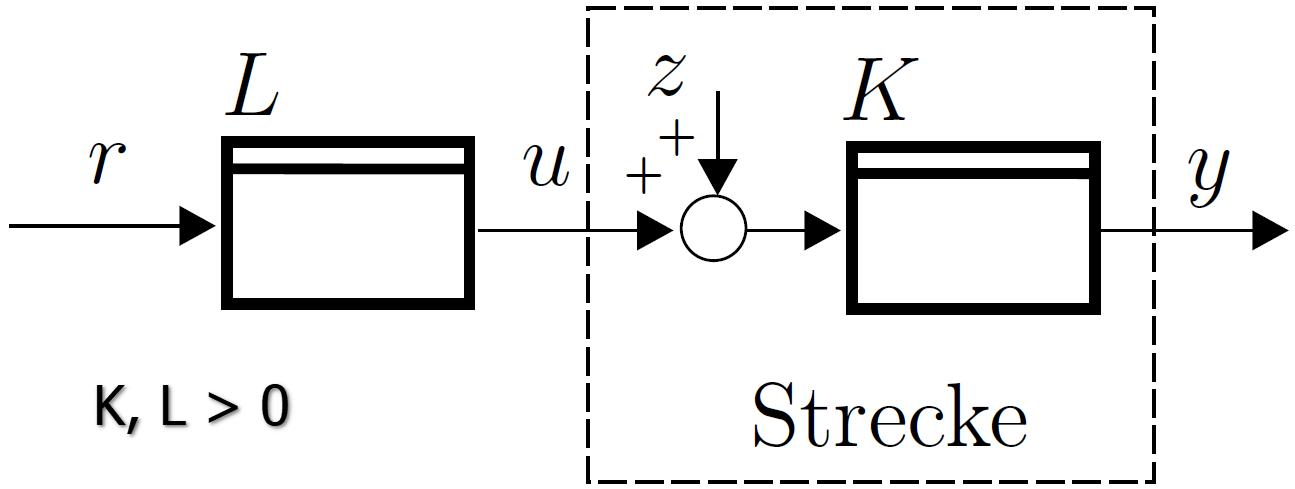
\includegraphics[align=center, width=\columnwidth]{images/steuerung.jpg}
    \end{minipage}
    \hfill
    \begin{minipage}[c]{0.5\columnwidth}
        Eine Steuerung besitzt \textbf{keine Rückkopplung} und ist somit ein \textbf{offener Regelkreis}
        $$ y = \underbrace{K L \cdot r}_{\text{Sensitivität}} + \underbrace{K \cdot z}_{\text{Störung}}$$
    \end{minipage}


\subsection{Regelung}

    \begin{minipage}[c]{0.48\columnwidth}
        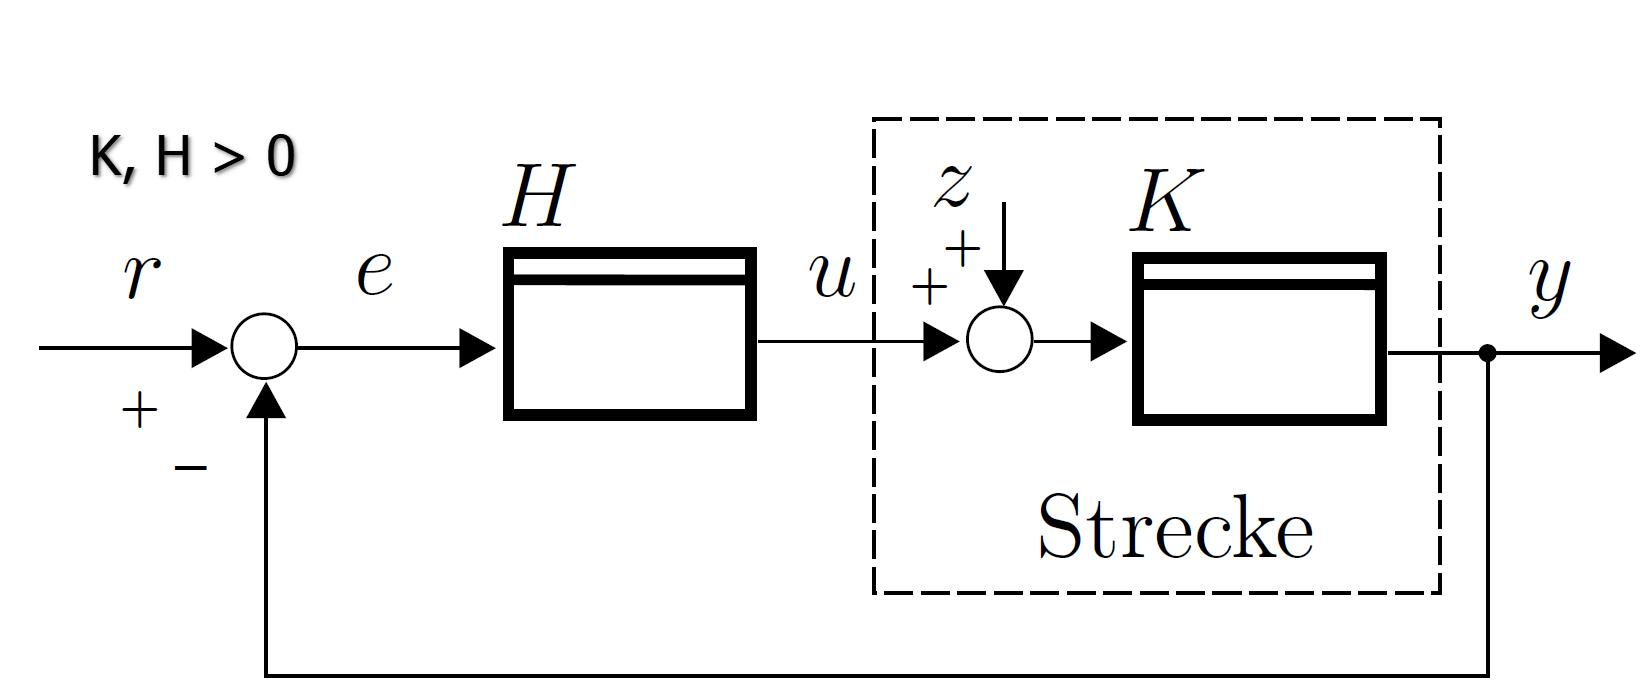
\includegraphics[align=center, width=\columnwidth]{images/regelung.jpg}
    \end{minipage}
    \hfill
    \begin{minipage}[c]{0.5\columnwidth}
        Eine regelung besitzt eine \textbf{Gegenkopplung}
        $$ y = K H \cdot (r - y) + K \cdot z$$
        $$ y = \underbrace{\frac{K H}{1 + K H} \cdot r}_{\text{Sensitivität}} + \underbrace{\frac{K}{1 + K H} \cdot z}_{\text{Störungsunterdrückung}} $$
    \end{minipage}


\subsubsection{Störungsunterdrückung}{106}

    Ein Regler ist vorteilhaft, um Störungen zu unterdrücken, denn für die Verstärkung der Störung $z$ gilt:
    $$ \lim\limits_{H \to \infty} \frac{K}{1 + K H} \cdot z = 0 $$
    \textrightarrow\ Hat der Regler eine grosse Verstärkung $H$, so wird die Störung $z$ unterdrückt\\
    \textrightarrow\ Bei einer Steuerung wird die Störung nicht unterdrückt


\subsubsection{Sensitivität (Empfindlichkeit)}{106}

    Für die Sensitivität eines Reglers gilt:
    $$ \lim\limits_{H \to \infty} \frac{K H}{1 + K H} \cdot r = 1 $$
    \textrightarrow\ Hat der Regler eine grosse Verstärkung $H$, so ist $y \approx r$ (Ausgang $\approx$ Sollwert)\\
    \textrightarrow\ Bei einer Steuerung muss $H = \frac{1}{L}$ sein, damit $y \approx r$


\subsubsection{Stabilitätsproblem}{109-110}

    Sobald ein offener Regelkreis (Steuerung) geschlossen wird, muss darauf geachtet werden, dass das System stabil ist.
    

\subsection{Stabilität eines Systems mit Rückkopplung}

    \begin{tabular}{lll}
        (asymp.) stabil     & Verstärkung $|V| < 1$ & System schwingt nicht \\
        grenzstabil         & Verstärkung $V = -1$  & System schwingt mit konstanter Ampl.\\
        instabil            & Verstärkung $|V| > 1$ & System schwingt mit zunehmender Ampl. 
    \end{tabular}


\subsubsection{Berechnung Grenzstabilität}{111}

    Für Grenzstabilität muss für die Verstärkung des Systems gelten: $V = -1$ 


    \example{Grenzstabilität System aus I-Glied und Totzeitglied}

    \begin{center}
        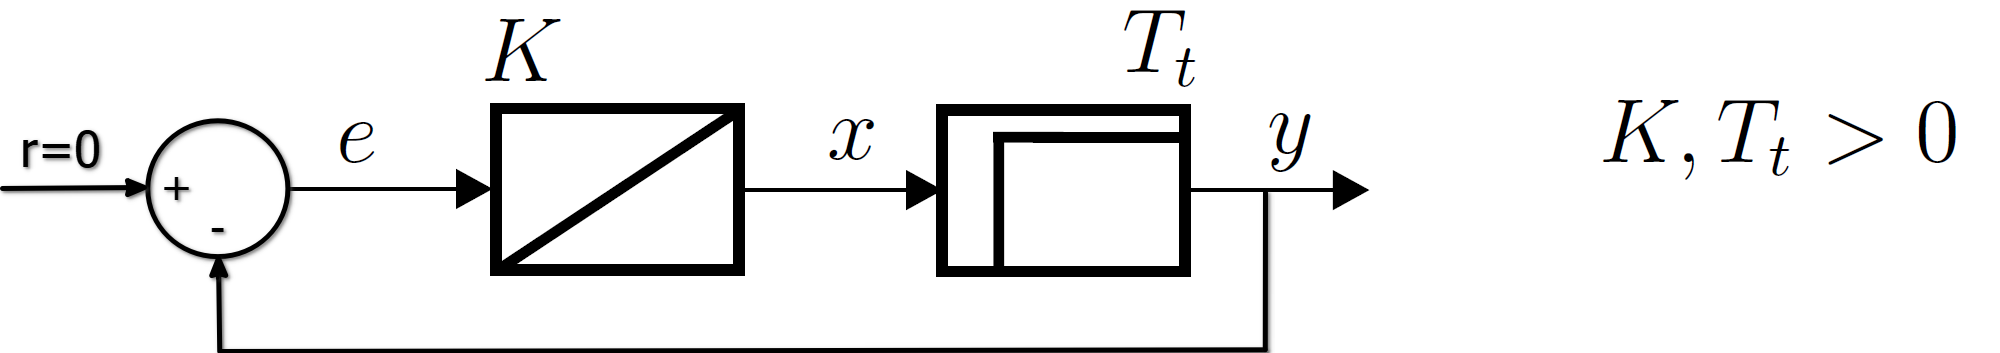
\includegraphics[align=center, width=0.75\columnwidth]{images/gegengekoppeltes_system.png}
    \end{center}

    Es muss gelten: $y(t) = -e(t)$ unter der Annahme, dass $e(t) = A \cdot \cos(\omega t)$

    \vspace*{-0.3cm}        % reduce space before align environment

    \begin{align*}
        x(t) &= K \cdot \int\limits_0^t e(\tau) \diff \tau + x_0 
            = K \cdot \int\limits_0^t A \cdot \cos(\omega \tau) \diff \tau + x_0
            = K \frac{A}{\omega} \sin(\omega \tau) \Big|_0^t + x_0 \\
            &= \frac{K A}{\omega} \sin(\omega t) + \underbrace{x_0}_{0} \\
        y(t) &= x(t - T_t) = \frac{K A}{\omega} \sin(\omega (t - T_t)) = \frac{K A}{\omega} \cos \big( \omega( t- T_t) - \frac{\pi}{2}  \big)
    \end{align*}

    Koeffizientenvergleich: 

    $$ \underbrace{ \cbl{ \frac{K A}{\omega}} \cos \big( \omega t \cor{- \omega T_t - \frac{\pi}{2}}  \big) }_{y(t)}
         = - A \cos(\omega t) = \underbrace{ \cbl{A} \cdot \cos(\omega t \cor{- \pi}) }_{-e(t)} $$
    
    \textrightarrow\ Wenn der Regler die Verstärkung $K$ hat ist das System grenzstabil 
    und das System schwingt für alle Zeit mit der Frequenz $\omega$\\
    \textrightarrow\ Die Verstärkung $K$ muss vermieden werden!
        % \section{Frequenzgang}{114} 

Wird ein Sinus-Signal $u(t)$ in ein LZI-System gegeben, so ist das Ausgangssignal $y(t)$ wieder sinusförmig.
Dabei ändern sich meist die \textbf{Amplitude} und die \textbf{Phase}.
Die \textbf{Frequenz} hingegen bleibt \textbf{gleich}.\\
Die Amplitude und die Frequenz des Ausgangssignals (bzw. deren Änderung) kann allerdings frequenzabhängig sein!

\begin{minipage}[c]{0.48\columnwidth}
    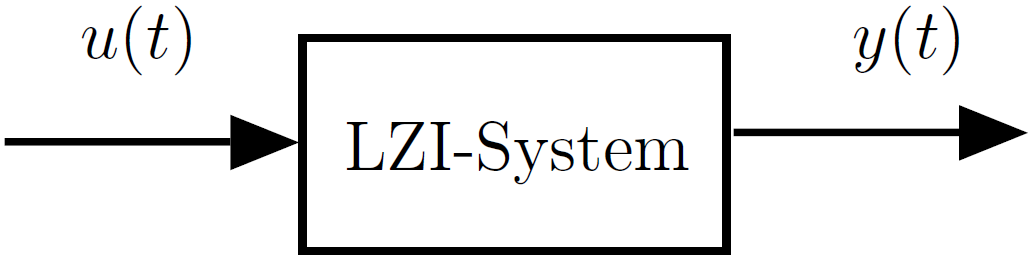
\includegraphics[width=\columnwidth]{images/lzi_system.png}
\end{minipage}
\hfill
\begin{minipage}[c]{0.48\columnwidth}
    \begin{tabular}{ll}
        $A$             & Amplitude Eingangssignal \\
        $B$             & Amplitude Ausgangssignal \\
        $\frac{B}{A}$   & Verstärkung \\
        $\varphi$       & Phasenverschiebung \\
    \end{tabular}
\end{minipage}

\fbox{\parbox{0.8\columnwidth}{
\begin{tabular}{l c l}
    $ u(t) = A \cdot \cos(\omega t) $ & & $ y(t) = B \cdot \cos(\omega t + \varphi) + \text{Transiente} $
\end{tabular}
}}

\subsubsection{Transiente}

 Die Transiente beschreibt den Vorgang, bis der eingeschwungene Zustand (\textbf{steady state}) erreicht ist.
 In der Praxis betrachtet man häufig $t = 5 \tau$ als Ende des Einschwingvorgangs \\
 \textrightarrow\ \textbf{Uns interessiert nur der der steady state!}


\subsubsection{Darstellung des Frequenzgangs}

% Der Frequenzgang stellt die Informationen zu einem System im Frequenzbereich dar. Es handelt sich hierbei um dieselben Informationen
% wie im Zeitbereich. Allerdings sind die Berechnungen im Frequenzbereich wesentlich einfacher als im Zeitbereich \\
Der Frequenzgang kann mittels folgenden Diagrammen dargestellt werden: 

\begin{itemize}
    \item Nyquist-Plot (Ortskurve)
    \item Bode-Plot
    \item Zeiger-Diagramm % stimmt das? 
\end{itemize}


\subsection[Frequenzgang G(j omega) als komplexe Zahl]{Frequenzgang $G(j \omega)$ als komplexe Zahl}{116}

\vspace{-0.3cm} % reduce space 
$$ \boxed{ G(j \omega) = |G(j \omega)| \cdot e^{j \angle G(j \omega)} = \frac{B}{A} \cdot e^{j  \varphi} } $$


\subsection{Frequenzgang der Grundglieder}

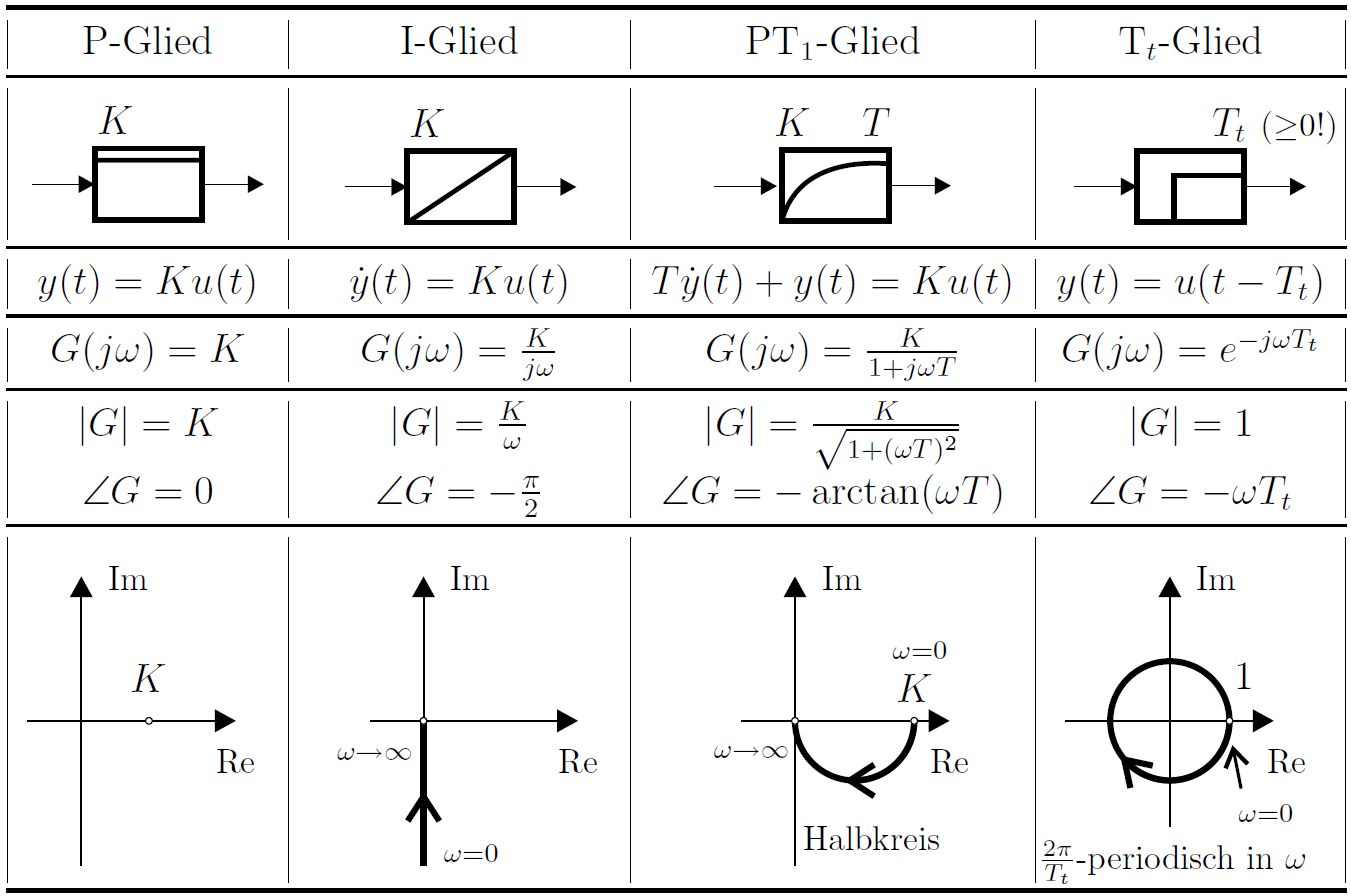
\includegraphics[width=\columnwidth]{images/frequenzgaenge_grundglieder.png} \\
\textrightarrow\ Zusammengesetzte Grundglieder: siehe Skript S. 204-208


\subsection{Darstellung mit Zeigern}

Im Frequenzbereich kann ein Signal \textbf{bei einer bestimmten Frequenz} als Zeigerdiagramm dargestellt werden.
Dabei wird das Signal $\underline{y}(t)$ als Zeiger $\underline{Y}$ zur Zeit $t=0$ dargestellt, welcher anschliessend mit Frequenz $\omega = 2 \pi f$ rotiert.
Das zeitliche Signal $y(t)$ entspricht dem \textbf{Realteil} von $\underline{y}(t)$

\begin{minipage}[c]{0.4\columnwidth}
    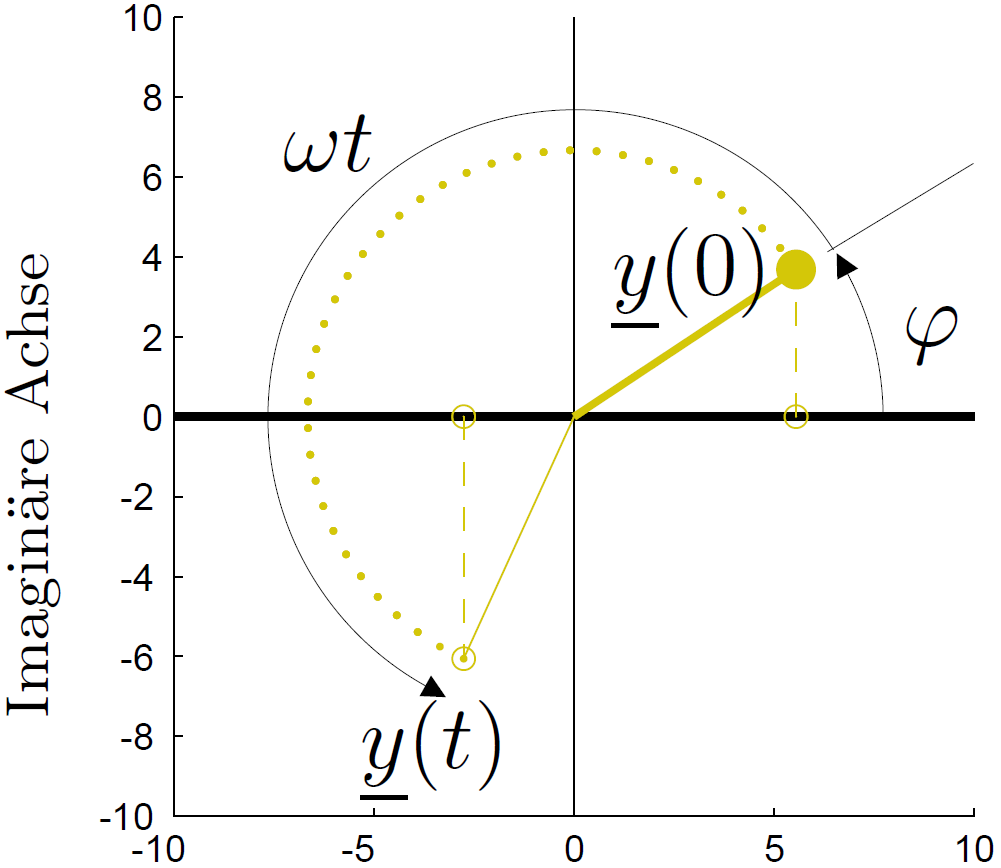
\includegraphics[width=\columnwidth]{images/zeigerdiagramm_1.png}
\end{minipage}
\hfill
\begin{minipage}[c]{0.4\columnwidth}
    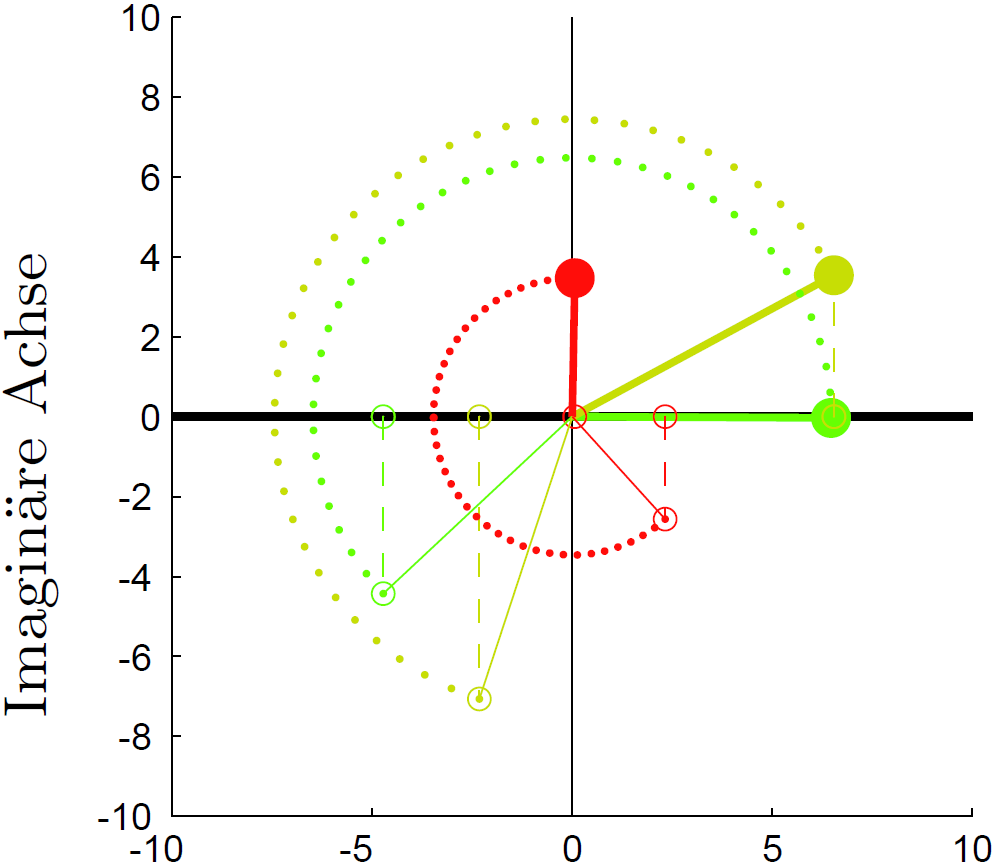
\includegraphics[width=\columnwidth]{images/zeigerdiagramm_2.png}
\end{minipage}


\subsubsection{Komplexe Amplitude $Y$}

\vspace{-0.5cm} % reduce space before align environment
\begin{align*}
    \underline{y}(t) &= B \cdot [\cos(\omega t + \varphi) + j \sin(\omega t + \varphi)] \\
                &= B \cdot e^{j(\omega t + \varphi)} = \cbl{B \cdot e^{j \varphi}} \cdot e^{j \omega t} \\
                &= \cbl{\underline{Y}} \cdot e^{j \omega t}
\end{align*}

Die in der Gleichung vorkommenden Grössen sind definiert als \\
\begin{tabular}{lll}
    $ | \underline{y}(t) | = B$                 & Maximale Amplitude des Ausgangssignals \\
    $ \mathrm{Re}(\underline{y}(t)) = y(t)$     & Ausgangssignal (zeitlich) \\
    $ \underline{y}(0) = \cbl{\underline{Y}} $  & Anfangszeiger (komplexe Amplitude)
\end{tabular}


\subsubsection{Ableitung / Integral im Frequenzbereich}

\begin{minipage}[c]{0.48\columnwidth}
    $$ \boxed{ \underline{\dot{y}}(t) = \underline{Y} \cdot j \omega \cdot e^{j \omega t} } $$
\end{minipage}
\hfill
\begin{minipage}[c]{0.48\columnwidth}
    $$\boxed{ \int y(t) \, \diff t = \frac{\underline{Y}}{j \omega} \cdot e^{j \omega t} } $$
\end{minipage}


\subsection{Bestimmung des Frequenzgangs aus DGL}

\begin{enumerate}
    \item DGL des Systems in Frequenzbereich transformieren
    \item Geeignet umformen: $G(j \omega) = \frac{\underline{Y}}{\underline{U}}$
    \item Falls gewünscht: Amplitude $|G(j \omega)|$ und Phase $\varphi$ bestimmen
\end{enumerate}


\example{$\text{PT}_1$ Glied}

\vspace{-0.3cm} % reduce space
$$ T \dot{y} + y(t) = K u(t) \quad \underrightarrow{\text{Frequenzbereich}} \quad 
T \cdot j \omega \cdot \underline{Y} + \underline{Y} = [j \omega T + 1] \cdot \underline{Y} = K \underline{U} $$
$$ \frac{\underline{Y}}{\underline{U}} = \frac{K}{j \omega T + 1} = G(j \omega) $$
$$ |G(j \omega)| = \frac{|\underline{Y}|}{|\underline{U}|} = \frac{K}{\sqrt{(\omega T)^2 + 1^2}} \qquad \varphi = \frac{K}{1 + (\omega T)^2} - j \frac{K \omega T}{1 + (\omega T)^2 } + \pi $$


\subsubsection{Allgemeiner Fall}


\vspace{-0.5cm} % reduce space before align environment
\begin{align*}
    a_n y(t)^{(n)} + \cdots  + a_1 \dot{y}(t) + a_0 y(t) &= b_m u(t)^{(m)} + \cdots + b_1 \dot{u}(t) + b_0 u(t) \\
    a_n (j \omega)^n \cdot \underline{Y} + \cdots + a_1 j \omega \cdot \underline{Y} + a_0 \underline{Y} 
    &=  b_m (j \omega)^m \cdot \underline{U} + \cdots + b_1 j \omega \cdot \underline{U} + b_0 \underline{U} \\
    \frac{\underline{Y}}{\underline{U}} 
    &= \frac{b_m (j \omega)^m + \cdots + b_1 j \omega + b_0}{a_n (j \omega)^n + \cdots + a_1 j \omega + a_0} = G(j \omega) \\
    |G(j \omega)| = \frac{|\underline{Y}|}{|\underline{U}|}
    &= \frac{| b_m (j \omega)^m + \cdots + b_1 j \omega + b_0 |}{| a_n (j \omega)^n + \cdots + a_1 j \omega + a_0 |} \\
    \varphi = \angle G(j \omega) &= \arctan \Big( \frac{\mathrm{Im} \{G(j \omega)\}}{\mathrm{Re}\{G(j \omega)\}} \Big) (+ \pi)
\end{align*}




\subsection{Serieschaltung von LZI-Systemen}

\begin{center}
    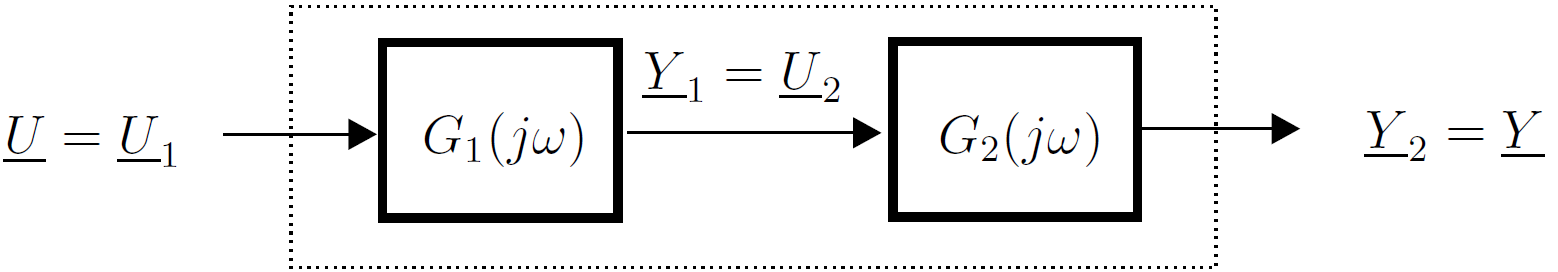
\includegraphics[width=0.7\columnwidth]{images/frequenzgang_serieschaltung.png}
\end{center}
$$ \boxed{ \underline{Y} = \underbrace{G_1(j \omega) \cdot G_2(j \omega)}_{G(j \omega)} \cdot \underline{U} } $$
$$ G_1 \dot G_2 = |G_1| \cdot e^{j \angle G_1} \cdot |G_2| \cdot e^{j \angle G_2} = |G_1| |G_2| \cdot e^{j (\angle G_1 + \angle G_2)} $$


\subsection{Parallelschaltung von LZI-Systemen}

\begin{center}
    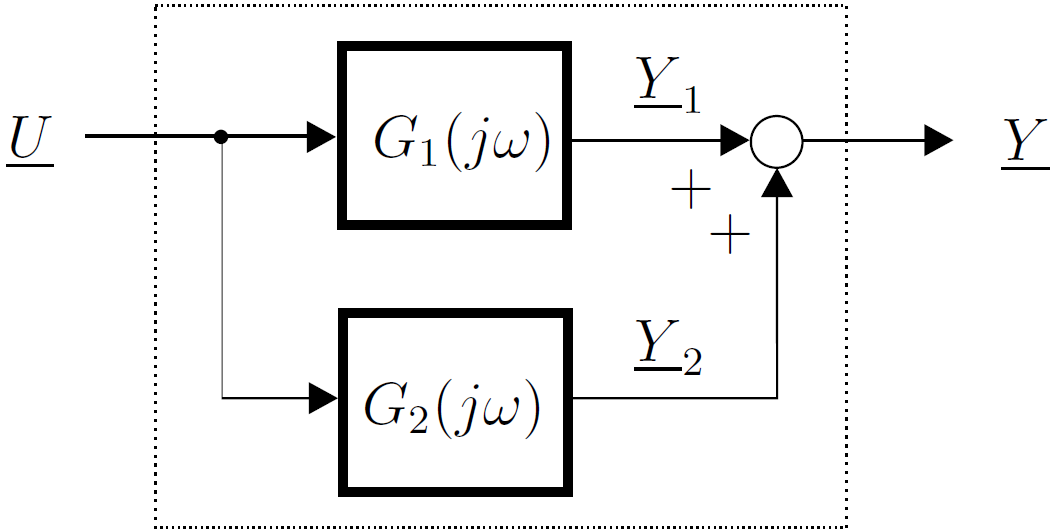
\includegraphics[width=0.5\columnwidth]{images/frequenzgang_parallelschaltung.png}
\end{center}
$$ \boxed{ \underline{Y} = \underline{Y}_1 + \underline{Y}_2 = G_1(j \omega) \cdot \underline{U} + G_2(j \omega) \cdot \underline{U} 
    = \underbrace{(G_1(j \omega) + G_2(j \omega))}_{G(j \omega)} \cdot \underline{U}} $$
$$ G_1 + G_2 = \mathrm{Re}\{ G_1 \} + \mathrm{Re}\{ G_2 \} + j ( \mathrm{Im}\{ G_1 \} + \mathrm{Im}\{ G_2 \}) $$


\subsection{Kreisschaltung (Gegenkopplung) von LZI-Systemen}

\begin{minipage}[c]{0.5\columnwidth}
    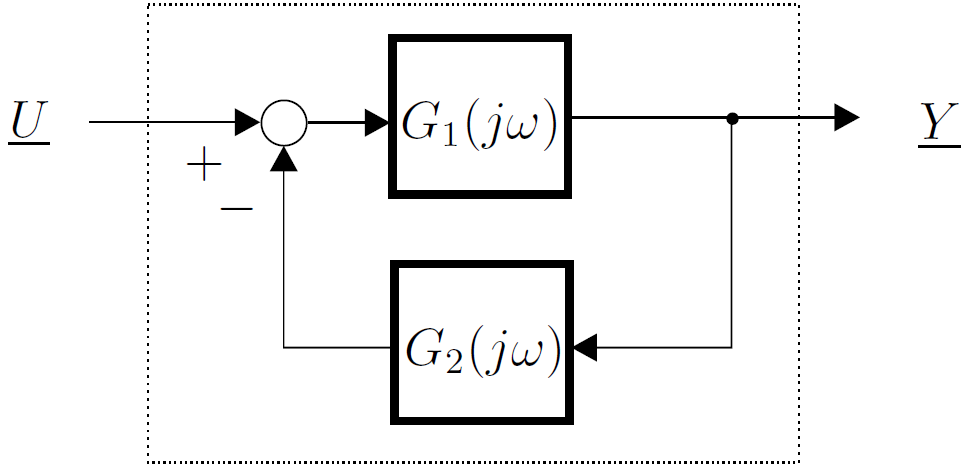
\includegraphics[width=\columnwidth]{images/frequenzgang_kreisschaltung.png}
\end{minipage}
\hfill
\begin{minipage}[c]{0.48\columnwidth}
    $$ \boxed{ \underline{Y} = \underbrace{\frac{G_1(j \omega)}{1 + G_1(j \omega) \cdot G_2(j \omega)}}_{G(j \omega)} \cdot \underline{U}} $$
    \textrightarrow\ Anwendung von \textbf{Mason Regel} (SigSys)
\end{minipage}


\subsubsection{Vorgehen Frequenzgang ermitteln}
\begin{enumerate}
    \item Gleichung zum Blockdiagramm aufstellen
    \item Nach $\underline{Y}$ umformen 
\end{enumerate}

\subsection{Frequenzgang -- Übertragungsfunktion (UTF)}

Der Frequenzgang $G(j \omega)$ und du Übertragungsfunktion $G(s)$ mit $s = \sigma + j \omega$ hängen folgendermassen zusammen:
$$ \boxed{G(j \omega) = G(s) \big\vert_{s = j \omega}} $$

\subsubsection{Übersicht Darstellungsformen}

\begin{center}
    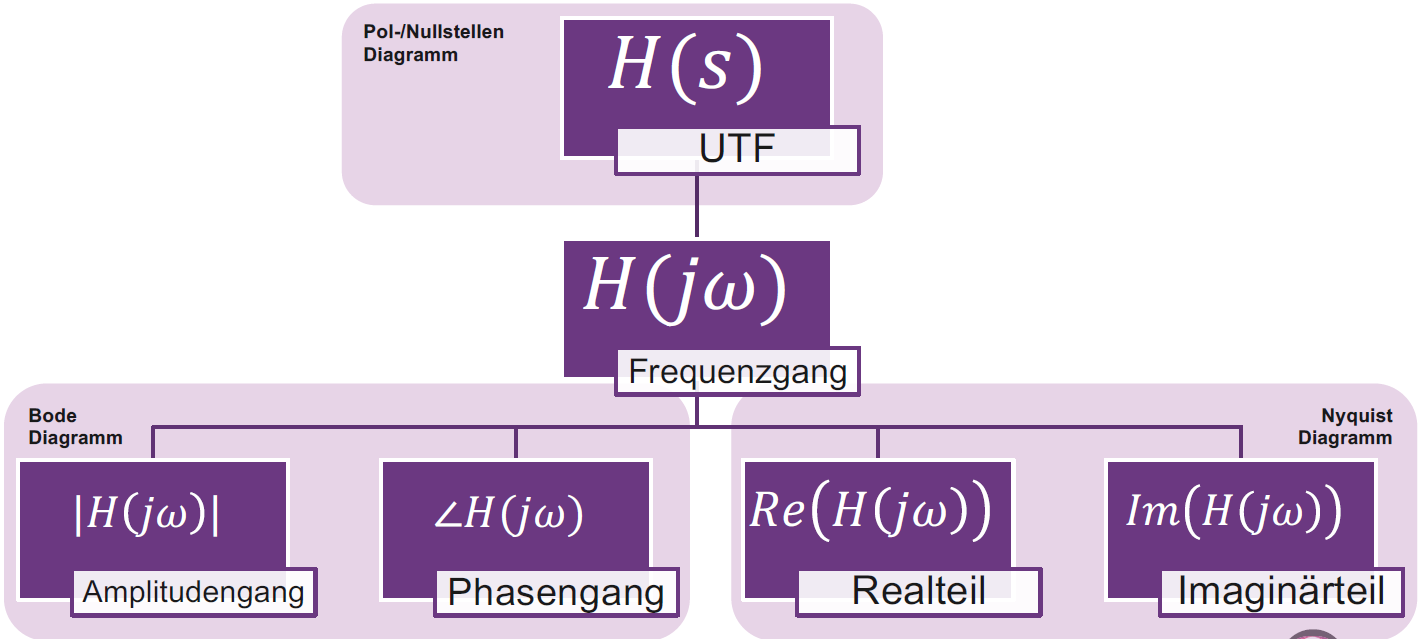
\includegraphics[width=0.75\columnwidth]{images/darstellungen_frequenzgang_utf.png}
\end{center}


        % \section{Stabilität -- Nyquistkriterium}{126}
\label{offener Regelkreis}

Die Stabilität eines Regelkreises kann mit dem Nyquistkriterium viel einfacher betrachtet werden. 
Dafür wird der \textbf{Frequenzgang} $\bm{G_0(\jimg \omega)}$ \textbf{des offenen Regelkreises} betrachtet.

Ausserdem gibt das Nyquistkriterium an, wie robust ein Regelkreis ist.

\begin{minipage}[c]{0.48\columnwidth}
    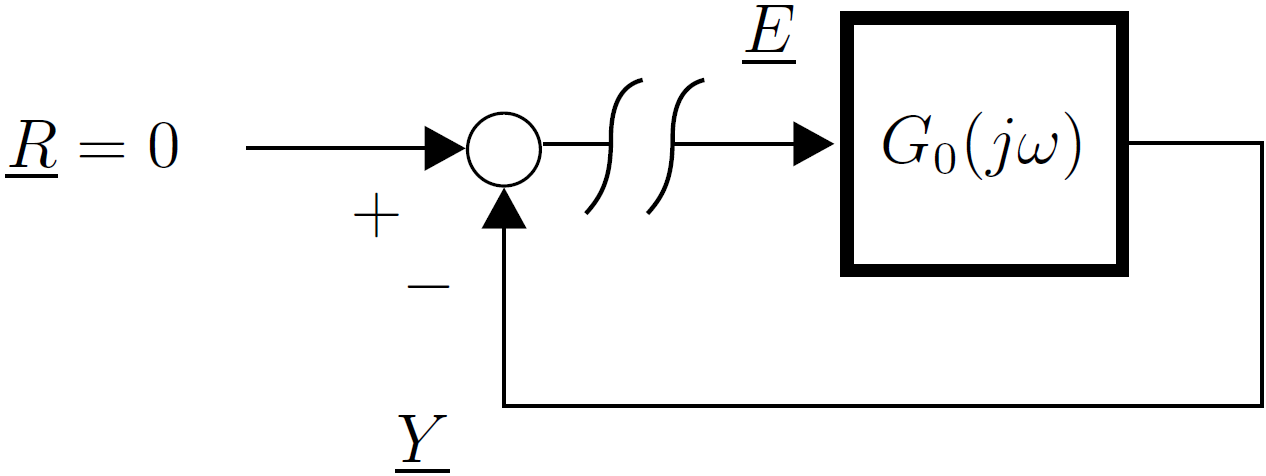
\includegraphics[width=\columnwidth]{images/offener_regelkreis.png}
\end{minipage}
\hfill
\begin{minipage}[c]{0.48\columnwidth}
    \begin{center}
        Frequenzgang des offenen Regelkreises
    \end{center}
    $$ \boxed{ G_0(\jimg \omega) = \frac{\underline{Y}}{\underline{E}} } $$
\end{minipage}



\example{Kreisschaltung mit mehreren Blöcken}
\label{Kreisschaltung mehrere Bloecke}

Folgendes System besitzt ein Eingangssignal $\underline{R}$ und vier Ausgangssignale $\underline{Y}$\\
Es sollen der Frequenzgang des offenen Regelkreises $G_0(\jimg \omega)$, sowie ausgewählte UTFs des Systems beschrieben werden.

$$ G_0(\jimg \omega) = G_1(\jimg \omega) \cdot G_2(\jimg \omega) \cdot G_3(\jimg \omega)  $$

\begin{minipage}[c]{0.5\columnwidth}
    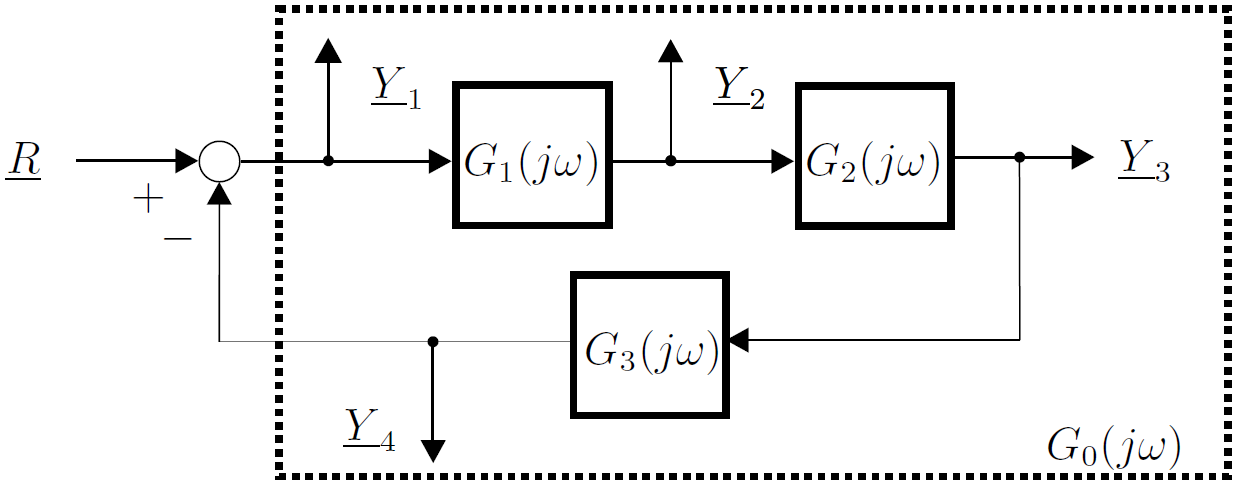
\includegraphics[width=\columnwidth]{images/kreisschaltung_mehrere_bloecke.png}
\end{minipage}
\hfill
\begin{minipage}[c]{0.48\columnwidth}
    $$ \frac{\underline{Y}_1}{\underline{R}} = \frac{1}{1 + G_1(\jimg \omega) \cdot G_2(\jimg \omega) \cdot G_3(\jimg \omega)} $$
    % $$ \frac{\underline{Y}_1}{\underline{R}} = \frac{G_1(\jimg \omega)}{1 + G_1(\jimg \omega) \cdot G_2(\jimg \omega) \cdot G_3(\jimg \omega)} $$
    $$ \frac{\underline{Y}_3}{\underline{R}} = \frac{G_1(\jimg \omega) \cdot G_2(\jimg \omega)}{1 + G_1(\jimg \omega) \cdot G_2(\jimg \omega) \cdot G_3(\jimg \omega)} $$
    % $$ \frac{\underline{Y}_4}{\underline{R}} = \frac{G_1(\jimg \omega) \cdot G_2(\jimg \omega) \cdot G_3(\jimg \omega)}{1 + G_1(\jimg \omega) \cdot G_2(\jimg \omega) \cdot G_3(\jimg \omega)} $$
\end{minipage}

\vspace{0.2cm}
\textbf{Hinweis:} Die Stabilität des Systems ist \textbf{unabhängig von der Reihenfolge der Teilsysteme} $G_{i}(\jimg \omega)$,
da die Stabilität durch den Nenner (bzw. die Polstellen) beschrieben wird.


\subsection{Stabilität im Nyquist-Diagramm}

Gedankenexperiment: Ein offener Regelkreis mit $G_0(\jimg \omega)$ (gemäss Abschnitt ~\ref{offener Regelkreis}) um eine 
veränderbare Verstärkung $K$ ergänzt.


\subsubsection{Stabilität}

Wähle $K = K_0$, sodass sich die Ortskurve immer innerhalb des Einheitskreises befindet.
\vspace{0.1cm}
\begin{itemize}
    \item Befindet sich die Ortskurve eines Systems immer \textbf{innerhalb des Einheitskreises}, so ist der offene Regelkreis stabil. \\
        \textrightarrow\ Daraus folgt, dass auch der geschlossene Regelkreis stabil sein muss.
    \item Führungsübertragungsfunktion für $K \ll K_0$:\\
    $G_f(\jimg \omega) = \frac{K \cdot G_0(\jimg \omega)}{1 + K \cdot G_0(\jimg \omega)} \approx K \cdot G_0(\jimg \omega)$ 
\end{itemize}


\subsubsection{Grenzstabilität}

Wähle $K = K_{\rm krit} > K_0$, sodass die Ortskurve den Punkt $-1$ schneidet.
\vspace{0.1cm}
\begin{itemize}
    \item Ortskurve des offenen Regelkreises $G_0(\jimg \omega)$ verläuft \textbf{durch den Punkt $\boldsymbol{-1}$}, 
    \item Die Frequenz $\omega_{\pi}$, für die $G_0(\jimg \omega_{\pi})= -1 = \e^{- \pi}$ heisst \textbf{kritische Frequenz}. Mit dieser 
        kritischen Frequenz schwingt das System.
    \item Die Führungsübertragungsfunktion $G_f(\jimg \omega) = \frac { K \cdot G_0(\jimg \omega)}{1 + K \cdot G_0(\jimg \omega)}$ wird bei 
    der kritischen Frequenz zu $G_f(\jimg \omega_{\pi}) = \frac{-1}{1-1} = - \infty $ \textrightarrow\ Grenzstabilität
\end{itemize}


\subsubsection{Instabilität}

Wähle $K > K_{\rm krit}$
\vspace{0.1cm}
\begin{itemize}
    \item Ortskurve verläuft nicht mehr durch den Punkt $-1$
    \item Das System ist instabil
\end{itemize}


\subsection{Vereinfachtes Nyquistkriterium}{127-128}

Idee: Informationen über den \textbf{offenen Regelkreis} verwenden, um die \textbf{Stabillität des geschlossenen Regelkreises} 
zu beurteilen


\subsubsection{Vereinfachtes Nyquistkriterium}

\fbox{\parbox{0.95\columnwidth}{
\begin{itemize}
    \item Gemäss Abschnitt ~\ref{Kreisschaltung mehrere Bloecke}  wird $G_0 = \prod_i G_i$ gebildet aus den seriegeschalteten
        Teilsystemen des offenen Regelkreises \cbl{(\textrightarrow\ Produkt aller $G_i$ \textbf{im Feedback-Loop})}
    \item $G_0$ muss dabei einem \textbf{Prozess mit Ausgleich \cbl{(stabilen Prozess)}} entsprechen; zusätzlich 
    \textbf{dürfen} noch einer oder zwei Integratoren seriegeschaltet sein\\
        Mit Polen formuliert: Bei $G_0$ sind maximal zwei Pole bei Null erlaubt; alle weiteren Pole müssen in der linken Halbebene liegen
    \item Damit der geschlossene Regelkreis stabil ist, muss der kritische Punkt $-1$ \textbf{links} der Nyquistkurve von $G_0$ liegen,
        wenn diese in Richtung zunehmender Frequenz durchlaufen wird ($\omega = 0 \ldots \infty$) 
        \cbl{\textrightarrow\ 'links der Kurve': Man befindet sich \textbf{auf der Kurve} und 'schaut' nach links und muss
        den Punkt $-1$ 'sehen'}
\end{itemize}
}}


\example{Ortskurven stabiler Systeme}{128}

\textbf{Achtung:} Damit die Stabilität der gezeigten Systeme beurteilt werden kann, muss sichergestellt werden, dass auch die ersten
beiden Punkte des vereinfachten Nyquistkriteriums eingehalten werden!

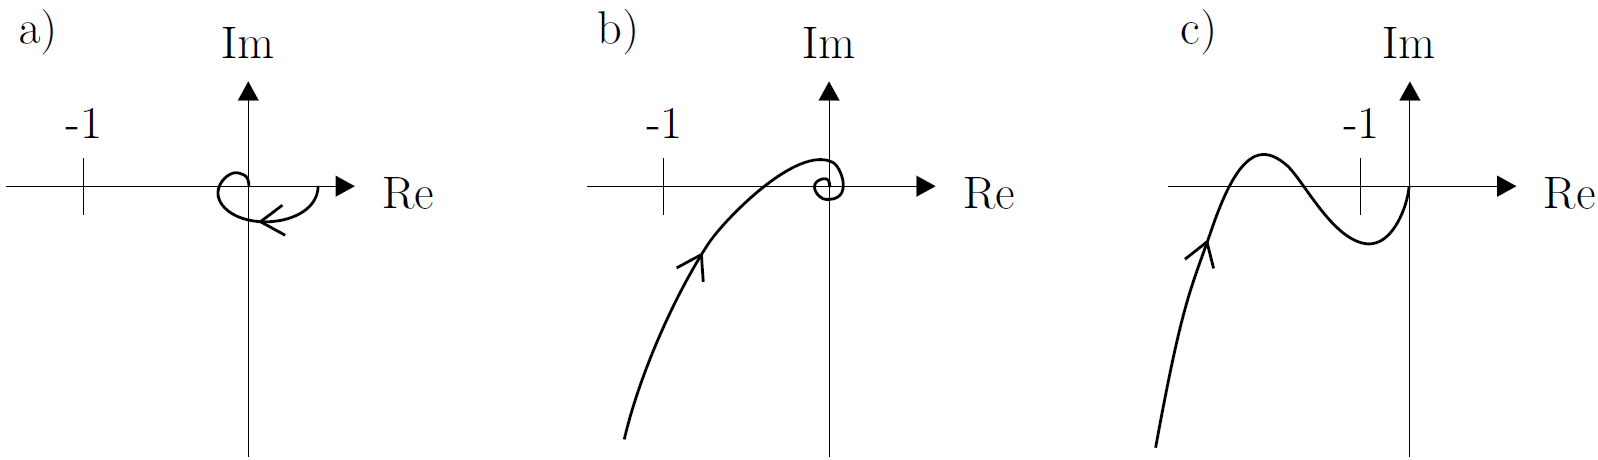
\includegraphics[width=\columnwidth]{images/nyquist_stabile_kurven.png}


\subsection{Stabilitätsreserven}

Wir möchten nicht nur Stabilität, sondern auch eine gewisse Stabilitätsreserve, um z.B. auch bei einem ungenau
modellierten Prozess oder einer sich ändernden Regelstrecke noch einen stabilen Regelkreis zu gewährleisten. 
\vspace{0.2cm}
\begin{outline}
    \1 \textbf{Auch ein stabiler Regelkreis kann sehr lange (ein)schwingen}
    \1 Stabilität / Grenzstabilität / Instabilität sind defnierte Bereiche
        \2 Es gibt nicht 'ein wenig stabil', 'ziemlich stabil', 'stabiler als...', 'instabiler als'
    \1 Allenfalls: Ein Regelkreis ist stabiler als ein anderer. Gemeint ist:
        \2 Ein Regelkreis ist besser gedämpft / schneller (eingeschwungen)
        \2 Ein Regelkreis ist robust -- er ist trotz gewissen Widerigkeiten im Regelkreis
        \2 \textbf{Ein Regelkreis bleibt stabil, auch wenn die Regelstrecke leicht ändert}
\end{outline}


\subsection{Stabilitätsreserven im Nyquistdiagramm}{129}


\begin{minipage}[c]{0.48\columnwidth}
    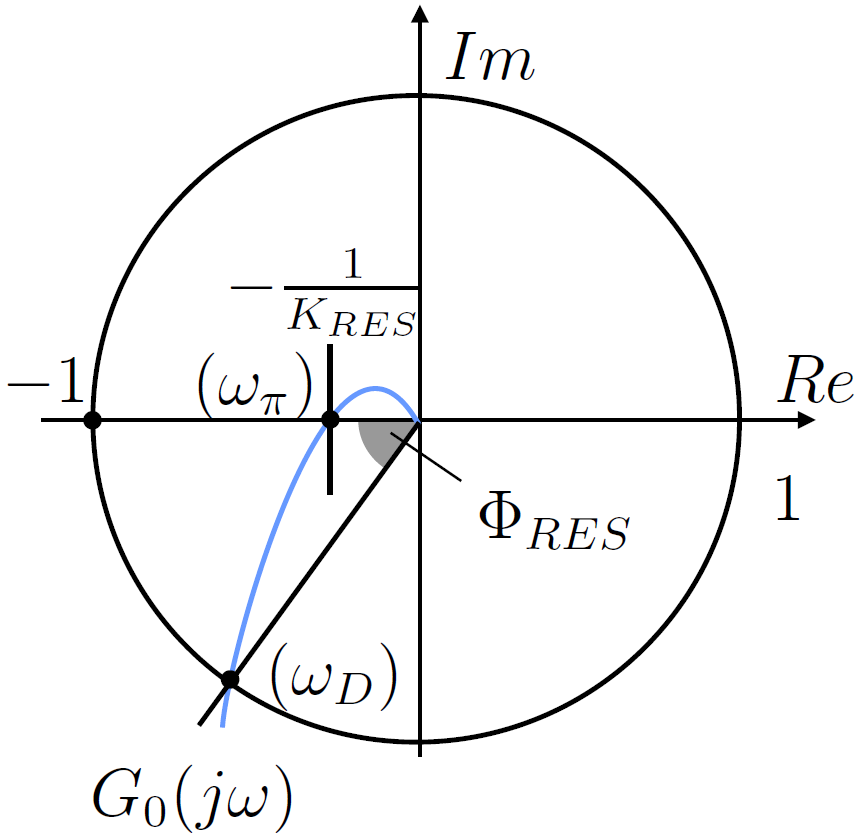
\includegraphics[width=\columnwidth]{images/stabilitaetsreserven_1.png}
\end{minipage}
\hfill
\begin{minipage}[c]{0.5\columnwidth}

    $$ \boxed{\Phi_{\rm RES} = \arctan \left( \frac{\Re{G_{0}(\jimg \omega_{D})}}{\Im{G_{0}(\jimg \omega_{D})}} \right) } $$
    $$ \boxed{\frac{1}{K_{\rm RES}} = \big| G_{0}(\jimg \omega_{\pi}) \big| } $$


     Ein System ist \textbf{stabil}, wenn eine der folgenden Bedingungen erfüllt ist:
     \vspace{0.2cm}

     \begin{itemize}
        \setlength\itemsep{4pt}
        \item $\omega_{\pi} > \omega_{D}$
        \item $G_{0}(\jimg \omega_{D}) = \e^{- \jimg \varphi}$ \quad mit $0 < \varphi < \pi$
        \item $0 > G_{0}(\jimg \omega_{\pi}) > -1 $
     \end{itemize}
\end{minipage}

\vspace{0.2cm}

\begin{itemize}
    \item Durchtrittsfrequenz $\omega_{D}$ \\
        Frequenz, bei der die Kurve den Einheitskreis durchquert: $| G_{0}(\jimg \omega_{D})| = 1 $ \\
        \textrightarrow\ Phasenreserve $\Phi_{\rm RES}$
    
    \item Phasenschnittfrequenz $\omega_{\pi}$ \\
        Frequenz, bei der die Kurve die reelle Achse durchquert: $\Im{G_{0}(\jimg \omega_{\pi})} = 0$\\
        \textrightarrow\ Verstärkungsreserve $K_{\rm RES}$
\end{itemize}


\subsubsection{Verstärkungsreserve $K_{\rm RES}$}

Die Verstärkungsreserve $K_{\rm RES}$ liefert direkt den Toleranzwert für den Fall, dass die \textbf{Modellunsicherheit} des 
offenen Regelkreises bei der \textbf{Verstärkung} liegt. \\
Der Abstand zur Ursprung bei der Phasenschnittfrequenz $\omega_{\pi}$ entspricht $\frac{1}{K_{\rm RES}}$ \\
\textrightarrow\ Wenn anstatt dem Nominalfrequenzgang $G_0(\jimg \omega)$ tatsächlich $K_{\rm RES} \cdot G_0(\jimg \omega)$ vorliegt, wird der
Regelkreis \textbf{grenzstabil}!


\subsubsection{Phasenreserve $\Phi_{\rm RES}$}

Die Phasenreserve $\Phi_{\rm RES}$ liefert einen Toleranzwert für den Fall, dass die \\
\textbf{Modellunsicherheit} des offenen Regelkreises bei der \textbf{Totzeit} liegt.

\textrightarrow\ Wenn anstatt dem Nominalfrequenzgang $G_0(\jimg \omega)$ tatsächlich $G_0(\jimg \omega) \cdot \e^{- \jimg \omega T_t}$ vorliegt, 
wird der Regelkreis \textbf{grenzstabil}!
\bigskip

Der Zusammenhang zwischen Phasendrehung und Totzeit ist
$$ \boxed{ T_t = \frac{\Phi_{\rm RES}}{\omega_D}  \quad \text{ wobei } [\Phi_{\rm RES}] = \rad } $$


\example{Einfluss von Stabilitätsreserven auf Nyquistdiagramm}

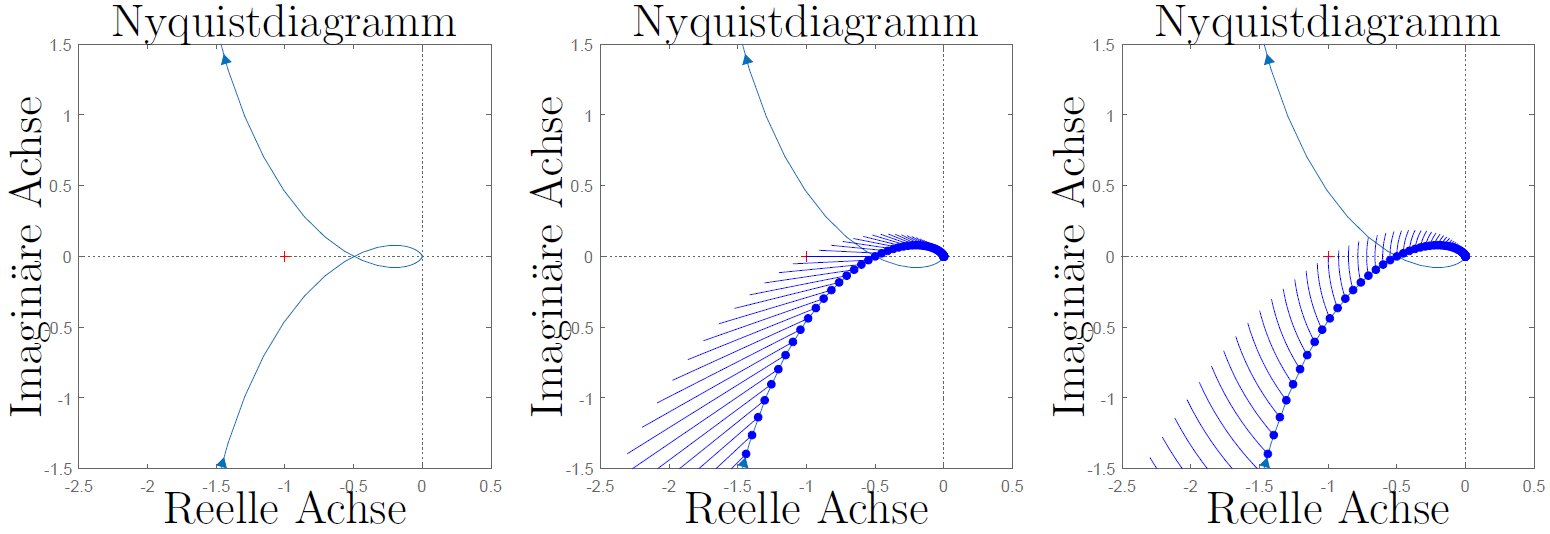
\includegraphics[width=\columnwidth]{images/nyquist_stabilitaetsreserven.png}

\begin{tabular}{ll}
    Mitte:  & Verstärkungsreserve streckt Kurve vom Ursprung aus \\
    Rechts: & Phasenreserve dreht jeden Punkt der Kurve um verschiedene Winkel $\omega \cdot T_t$ \\
            & um den Ursprung  
\end{tabular}


\subsubsection{Faustregeln für Reserven}{131}

\textbf{Hinweis:} Es besteht eine Kopplung zwischen den beiden Effekten!

\begin{itemize}
    \item Phasenreserve von $\Phi_{\rm RES} = 40 \degree \ldots 70 \degree$
    \item Verstärkungsreserve von $K_{\rm RES} > 4 \, (\approx 12 \, \deci \bel)$
\end{itemize}


\subsection{Nyquistdiagramme mit MatLab}

\lstinputlisting{snippets/nyquist.m}


\subsection{Vorgehen: Nyquistdiagramme zeichnen}

\begin{itemize}
    \item Werte für $G(\omega = 0)$ und $G(\omega = \infty)$ berechnen
    \item Anzahl $\jimg$ im Zähler \textbf{plus} Anzahl $\jimg$ im Nenner entspricht Anzahl Quadranten, welche zwischen $\omega = 0$ und 
        $\omega = \infty$ durchlaufen werden
    \item Pollstellen: $|G(\jimg \omega)|$ \textdownarrow\ ; $\angle G(\jimg \omega)$ \textdownarrow\ \textrightarrow\ Bewegung im Uhrzeigersinn
        \textrightarrow\ Bei den Nullstellen ist $\angle G(\jimg \omega) = \pm 45 \, \degree$
    \item Nullstellen: $|G(\jimg \omega)|$ \textuparrow\ ; $\angle G(\jimg \omega)$ \textuparrow\ ; \textrightarrow\ Bewegung im Gegenuhrzeigersinn
    \item Frequenzen der Pol- bzw. Nullstellen berechnen
\end{itemize}


        % \section{Dezibel $\deci \bel$}


\subsection{Umrechnung Verstärkungsfaktor -- Dezibel $\deci \bel$}

$$ \boxed{ |K|_{\deci \bel} = 20 \, \deci \bel \cdot \log_{10} |K| \quad \Leftrightarrow \quad 
            |K| = 10 ^{\big( \frac{|K|_{\deci \bel}}{20 \, \deci \bel}\big)}  } $$

Hinweis: Die Betragsstrichte sind Notation! Es können sehr wohl negative Werte entstehen!

\subsubsection{Rechenregeln}

\begin{itemize}
    \item Multiplikation \textrightarrow\ Addition
    \item Division \textrightarrow\ Subtraktion
    \item Kehrwert \textrightarrow\ Negatives Vorzeichen
\end{itemize}


\subsection{$\deci \bel$--Umrechnungstabelle}

% copy paste from SigSys -> to be updated
\begin{ctabular}{l l}
    \toprule
    \textbf{Dezibel}        & \textbf{Faktor} \\
    \midrule
    $20 = 10 + 10$          & $100 = 10 \cdot 10$ \\ 
    $12$                    & $16 = 2 \cdot 2 \cdot 2 \cdot 2$ \\
    $\cor{10}$              & $\cor{10}$ \\
    $9 = 3 + 3 + 3$         & $8 = 2 \cdot 2 \cdot 2$ \\
    $8 = 5 - 3$             & $6.4 = 3.2 \cdot 2$ \\
    $7 = 10 -3$             & $5 = \frac{10}{2}$ \\
    $6 = 3 + 3$             & $4 = 2 \cdot 2$ \\
    $5 = 15 - 10$           & $3.2 = \frac{32}{10\mathstrut} \approx \sqrt{10}$ \\
    $4 = 10 - 6 = 10 - 3-3$ & $2.5 = \frac{10\mathstrut}{2 \cdot 2}$ \\
    $\cor{3}$               & $\cor{2}$ \\
    $2= 12-10= 5-3$         & $1.6 = \frac{16}{10}$ \\
    $1 = 10 - 3 - 3 - 3$    & $1.25 = \frac{10}{2\cdot 2 \cdot 2} = \frac{5}{4}$ \\
    $\cor{0}$               & $\cor{1}$ \\
    $-1$                    & $0.8 = \frac{4}{5}$ \\
    \bottomrule
\end{ctabular}

        % \section{Bode-Diagramm}

Das Bode-Diagramm ist eine weitere Variante, den Frequenzgang $G(\jimg \omega)$ grafisch darzustellen.
Die Darstellung beinhaltet zwei Graphen.

\begin{itemize}
    \item Amplitudengang $|G(\jimg \omega)|$ in Dezibel $\deci \bel$
    \item Phasengang $\angle G(\jimg \omega)$ in Grad $\degree$
    \item Die Frequenzachse ist \textbf{logarithmisch} mit $\log_{10}(\omega)$
    \item \textbf{Ein Bodediagramm kann in ein Nyquistdiagramm umgezeichnet werden, aber nicht umgekehrt!}
\end{itemize}


% Bei zu wenig Platz weglassen
\subsubsection{Logarithmische Frequenzachse}{134}

\begin{outline}
    \1 Serieschaltung von Systemen
        $$ G(\jimg \omega) = G_1(\jimg \omega) \cdot G_2(\jimg \omega) $$

        \2 Amplitudengang
            $$ |G(\jimg \omega)| = |G_1(\jimg \omega)| \cdot |G_2(\jimg \omega)| $$
            $$ |G(\jimg \omega)|_{\deci \bel} = |G_1(\jimg \omega)|_{\deci \bel} + |G_2(\jimg \omega)|_{\deci \bel} $$
            \textrightarrow\ Grafisch multiplizieren wäre schwierig, grafisch addieren geht gut

        \2 Phasengang
            $$ \angle G(\jimg \omega) = \angle G_1(\jimg \omega) +  \angle G_2(\jimg \omega) $$
            \textrightarrow\ Die Phase muss nicht logarithmisch sein, wir haben schon eine Addition 
\end{outline}


\subsection{Vorgehen: Bode-Diagramm zeichnen}
\label{Bodediagramm zeichnen}

Das Diagramm wird approximativ mit \textbf{Geraden} gezeichnet!

\begin{outline}
    \1 Frequenzgang in folgende Form bringen:
        $$ G(\jimg \omega) = K_0 \cdot (\jimg \omega)^v \cdot \frac{(1 + T_{n0} \cdot \jimg \omega)\cdot (1 + T_{n1} \cdot \jimg \omega) \cdot \ldots}
        {(1 + T_{p0} \cdot \jimg \omega)\cdot (1 + T_{p1} \cdot \jimg \omega) \cdot \ldots} \cdot e^{- \jimg \omega T_t} $$
        \2 Für $\omega = 0$ sind alle $(1 + T \cdot \jimg \omega) = 1 = 0 \, \deci \bel$
        \2 Für $\omega = \frac{1}{T}$ sind alle  $(1 + T \cdot \jimg \omega) = 1 + \jimg = \sqrt{2} \cdot e^{\jimg \frac{\pi}{4}} 
            = 3 \, \deci \bel \angle 45 \, \degree$
    \1 Frequenzen der Nullstellen berechnen: $\omega = \frac{1}{T_n}$
    \1 Frequenzen der Polstellen berechnen: $\omega = \frac{1}{T_p}$


    \1 Jede \textbf{Nullstelle} bewirkt
        \2 einen Knick um $+ 20 \, \deci \bel$ / Dekade \textbf{nach oben} im Amplitudengang
        \2 einen Phasenhub von $+ 90 \, \degree$ über 2 Dekaden \textrightarrow\ $+ 45 \, \degree$ beim Knick
    \1 Jede \textbf{Polstelle} bewirkt
        \2 einen Knick um $- 20 \, \deci \bel$ / Dekade \textbf{nach unten} im Amplitudengang
        \2 einen Phasenverlust von $- 90 \, \degree$ über 2 Dekaden \textrightarrow\ $- 45 \, \degree$ beim Knick
    \1 Einzelne Faktoren einzeichnen \textrightarrow\ Wenn Faktor quadriert ist, zwei mal einzeichnen!
    \1 Grafische Addition der Faktoren für gesamten Frequenzgang
\end{outline}


\example{Bode-Diagramm zeichnen}
\vspace{-0.2cm}
$$ G(\jimg \omega) = \frac{\jimg \omega + 10}{(\jimg \omega + 0.1)} \quad  \underrightarrow{\text{ Standardform }} \quad 
  G(\jimg \omega) = \cgn{100} \cdot \frac{(\cvt{1 + 0.1 \, \jimg \omega})}{(\cbl{ 1 + 10 \, \jimg \omega})} $$

  \begin{itemize}
    \item $ \cgn{\abs{K_0}_{\deci \bel} = \abs{100}_{\deci \bel} = 40 \, \deci \bel}$ \textrightarrow\ $\angle G(100) = 0 \, \degree$
    \item Nullstelle: \cvt{$\abs{1 + 0.1 \, \jimg \omega}_{\deci \bel}$} \textrightarrow\ Knick bei $\omega = \frac{1}{0.1 \, \second} = 10 \frac{\rad}{\second}$
    \item Polstelle: \cbl{$\abs{1 + 10 \, \jimg \omega}_{\deci \bel}$} \textrightarrow\ Knick bei $\omega = \frac{1}{10 \, \second} = 0.1 \frac{\rad}{\second}$
    \item \cor{Endresultat}: Grafische Addition der Teilresultate
  \end{itemize}

\begin{center}
    % Gain
    \begin{tikzpicture}
        [
            scale = 0.8,
            >=latex
        ]
        \begin{axis}
            [
                width=12cm,
                height=4cm,
                xmode=log,
                xmin=0.01, xmax=100, ymin=-40, ymax=60,
                x label style={anchor=west},
                xlabel=Frequency $\omega$,
                y label style={anchor=south},
                ylabel=Gain $\deci \bel$,
                xmajorgrids=true,
                xminorgrids=true,
                ymajorgrids=true
            ]
            
            % K_0
            \addplot[thick, color=green, domain=0.01:100]{40};

            % Nullstelle
            \addplot[thick, color=violet, domain=0.01:10]{0};               % start bis Knick
            \addplot[thick, color=violet, domain=10:100]{20*log10(x)-20};   % ab Knick nach oben    

            % Polstelle
            \addplot[thick, color=blue, domain=0.01:0.1]{0};                % start bis Knick
            \addplot[thick, color=blue, domain=0.1:100]{-20*log10(x)-20};   % ab Knick nach oben    
            
            % Grafische Addition
            \addplot[thick, color=orange, domain=0.01:0.1]{40};    
            \addplot[thick, color=orange, domain=0.1:10]{-20*log10(x)+20};        
            \addplot[thick, color=orange, domain=10:100]{0};      
           
        \end{axis}
        
    \end{tikzpicture}

    \vspace{0.3cm}


    % Phase
    \begin{tikzpicture}
        [
            scale = 0.8,
            >=latex
        ]
        \begin{axis}
            [
                width=12cm,
                height=4cm,
                xmode=log,
                xmin=0.01, xmax=100, ymin=-180, ymax=180,
                x label style={anchor=west},
                xlabel=Frequency $\omega$,
                y label style={anchor=south},
                ylabel=Phase $\degree$,
                ytick={-180, -90, 0, 90, 180},
                % yticklabels={-180, -90, 0, 90, 180},
                xmajorgrids=true,
                xminorgrids=true,
                ymajorgrids=true
            ]
            
            % K_0
            \addplot[thick, color=green, domain=0.01:100]{0};
                
            % Nullstelle
            % \addplot[thick, color=violet, domain=0.01:1]{0};              % start bis Knick
            % \addplot[thick, color=violet, domain=1:10]{};        % ab Knick nach oben    
            
            % Polstelle
            % \addplot[thick, color=blue, domain=0.01:0.1]{0};                % start bis Knick
            % \addplot[thick, color=blue, domain=0.1:100]{-20*log10(x)-20};   % ab Knick nach oben    
            
            % Grafische Addition
            % \addplot[thick, color=orange, domain=0.01:0.1]{40};    
            % \addplot[thick, color=orange, domain=0.1:10]{-20*log10(x)+20};        
            % \addplot[thick, color=orange, domain=10:100]{0};      


            
        \end{axis}
            
    \end{tikzpicture}
\end{center}


\subsubsection{Inverse Frequenzgänge}{137}

Um das Bodediagramm des inversen Frequenzgangs $\frac{1}{G(\jimg \omega)}$ zu erhalten, muss bei Betrag \textbf{und} Phase
das \textbf{Vorzeichen gedreht} werden.
\vspace{0.2cm}
 
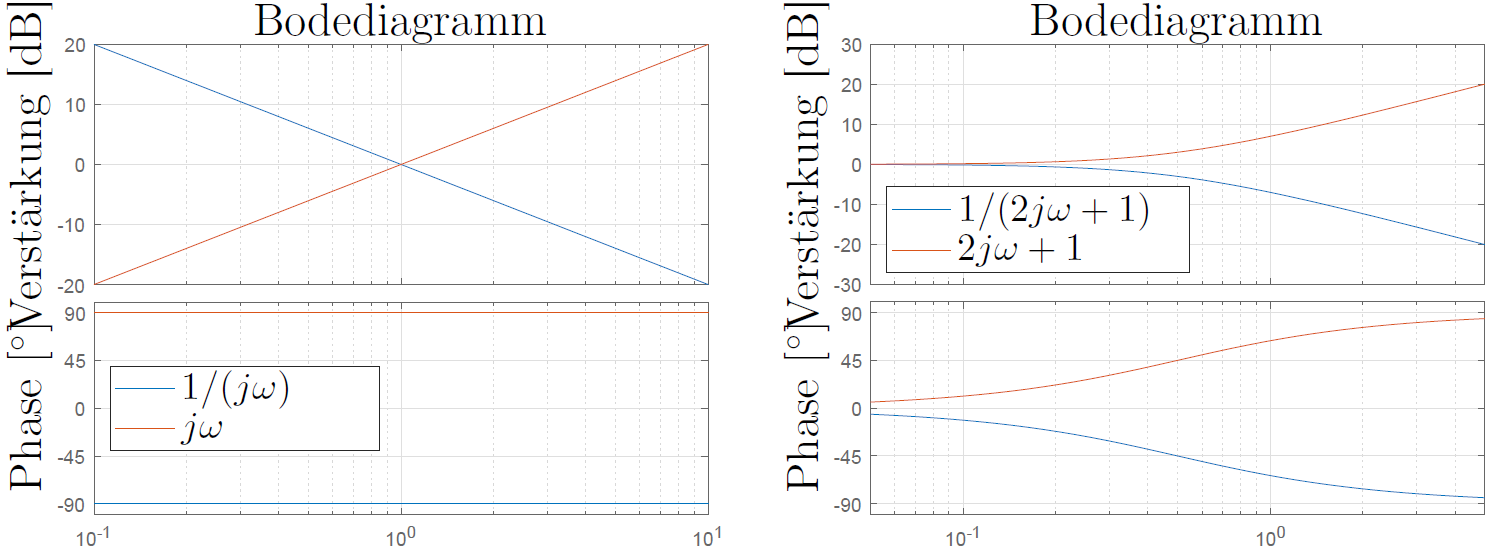
\includegraphics[width=\columnwidth]{images/inverse_frequenzgaenge.png}


\subsubsection{Lead-Lag-Glied}

$$ \boxed{ \text{Lead-Lag-Glied: } \quad G(s) = K \cdot \frac{s T_1 + 1}{s T_2 + 1} } $$

\begin{minipage}[c]{0.48\columnwidth}
    \begin{center}
        \myul{Lead-Glied ($T_1 > T_2$)}
    \end{center}
    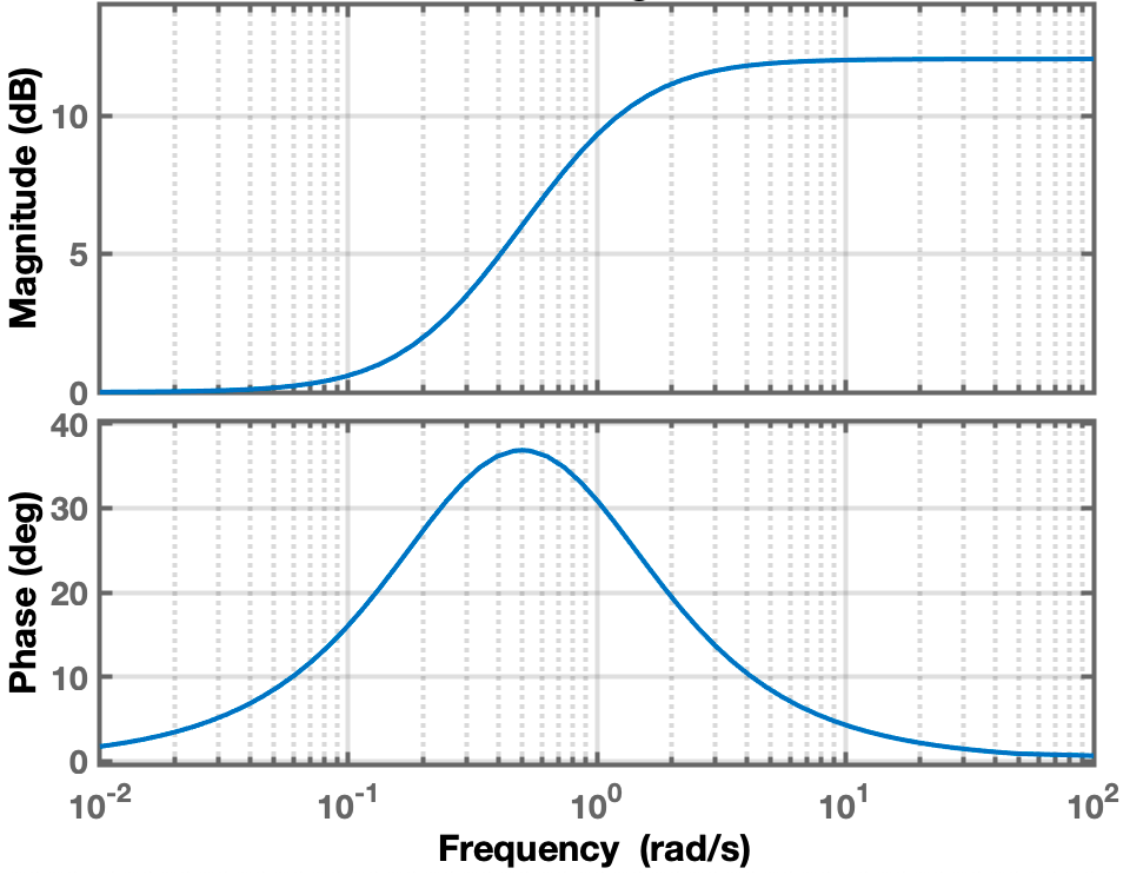
\includegraphics[width=\columnwidth]{images/bode_lead-glied.png}
\end{minipage}
\hfill
\begin{minipage}[c]{0.48\columnwidth}
    \begin{center}
        \myul{Lag-Glied ($T_2 > T_1$)}
    \end{center}
    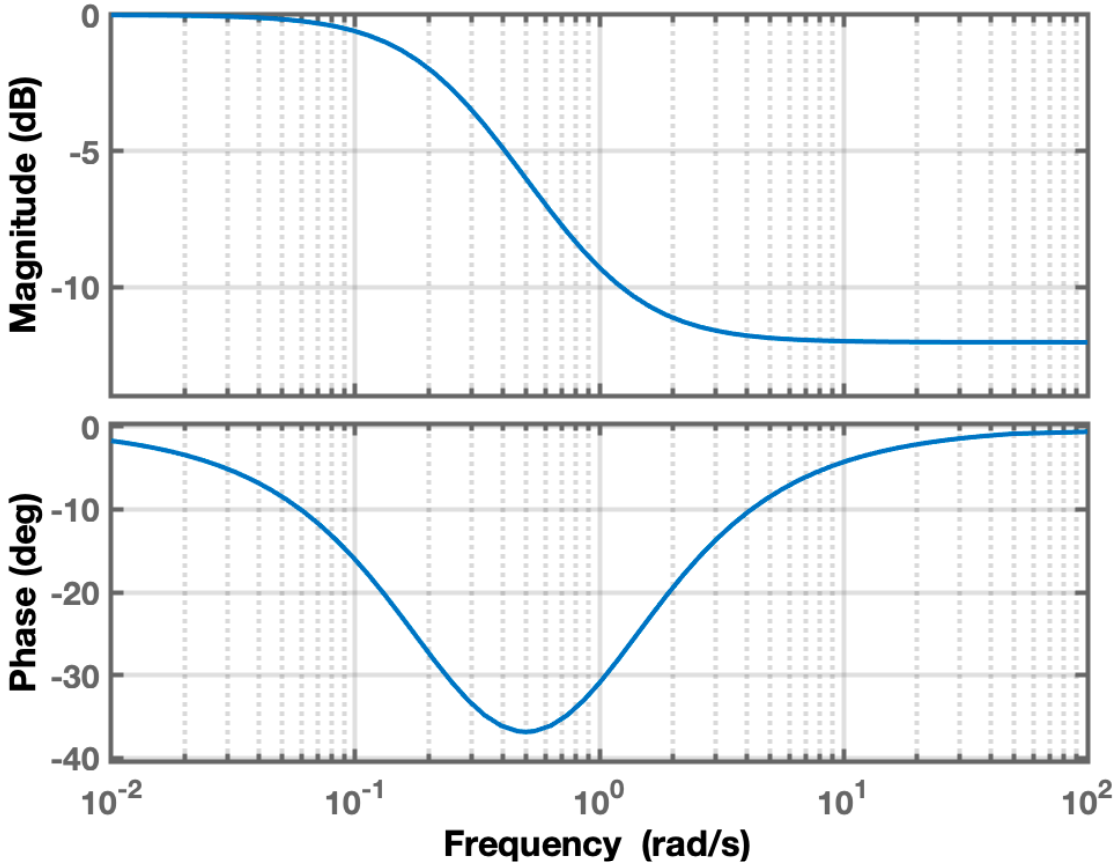
\includegraphics[width=\columnwidth]{images/bode_lag_glied.png}
\end{minipage}

$$ \boxed{ \text{Maximale Phasenänderung bei:} \quad \omega = \frac{1}{\sqrt{T_1 \cdot T_2}} } $$
\textrightarrow\ Bei der Regler-Auslegung werden vor allem Lead-Glieder verwendet, um \textbf{Phase anheben} zu können


\subsection{Modellbildung (UTF) mittels Frequenzmessung}{139}

Um aus einem gegebenen Bodediagramm die Übertragungsfuntion $G(\jimg \omega)$ zu ermitteln, werden die Zeichenregeln aus Abschnitt
~\ref{Bodediagramm zeichnen} \textbf{rückwärts angewendet}. Dazu werden die Punkte einer gegebenen Messung mittels Geraden approximiert.
Mittels dieser Approximationen können die einzelen Komponenten (Faktoren) der gesuchten UTF ermittelt werden.


\example{Übertragungsfuntion $G(s)$ aus Bodediagramm ermitteln}

\begin{minipage}[c]{0.5\columnwidth}
    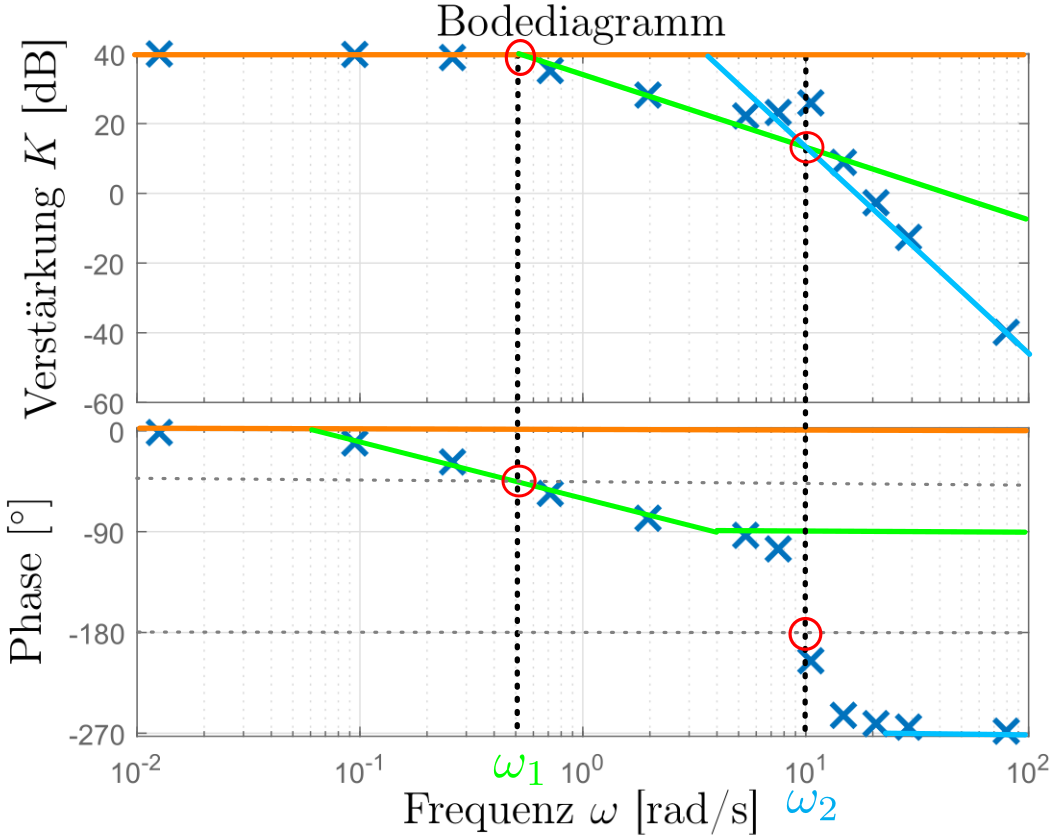
\includegraphics[width=\columnwidth]{images/bode_zu_modell.png}
\end{minipage}
\hfill
\begin{minipage}[c]{0.48\columnwidth}
    Aus den Steigungen der Geraden ist ersichtlich, dass folgende Komponenten in $G(s)$ enthalten sein müssen: \\
    \cor{Verstärkung $K$}, \cgn{$\text{PT}_1$-Glied}, \textcolor{cyan}{$\text{PT}_2$-Glied}
    $$ G(s) = \cor{K} \cdot \cgn{\frac{1}{(s T_1 + 1)}} \cdot \textcolor{cyan}{\frac{1}{(T_2^2 s^2 + 2 \zeta T_2 s + 1)}} $$
    Werte der Parameter aus Bodediagramm bestimmen:
    \begin{itemize}
        \item \cor{$|K|_{\deci \bel} = 40$ \textrightarrow\ $K = 100$}
        \item \cgn{$\omega_1 = \frac{1}{T_1} = 0.5$ \textrightarrow\ $T_1 = \frac{1}{0.5} = 2$}
        \item \textcolor{cyan}{$\omega_2 = \frac{1}{T_2} = 10$ \textrightarrow\ $T_1 = \frac{1}{10} = 0.1$}
        \item \textcolor{cyan}{$\zeta = 0.1$} \textrightarrow\ gegeben 
    \end{itemize}
\end{minipage}



\subsection{Stabilität im Bodediagramm}{140}
Analog zum Punkt $-1$ im Nyquistdiagramm kann die Stabilität auch im Bodediagramm beurteilt werden. Auch bei dieser Betrachtung 
sind die folgenden Frequenzen relevant.

\begin{itemize}
    \item Durchtrittsfrequenz $\omega_{D}$ \textrightarrow\ Phasenreserve $\Phi_{RES}$ \\
        Frequenz, bei der die Verstärkung 1 ist: $| G_{0}(\jimg \omega_{D})| = 1 \, (= 0 \, \deci \bel)$
    \item Phasenschnittfrequenz $\omega_{\pi}$ \textrightarrow\ Verstärkungsreserve $K_{RES}$ \\
        Frequenz, bei der die Phase $-180 \, \degree$ beträgt: $\angle {G_{0}(\jimg \omega_{\pi})} = - \pi \, \rad \, (= -180 \, \degree)$
\end{itemize}


\subsubsection[Parameter K_{RES} und  \Phi_{RES} aus Bodediagramm lesen]{Parameter $K_{RES}$ und  $\Phi_{RES}$ aus Bodediagramm lesen}

\begin{minipage}[c]{0.55\columnwidth}
    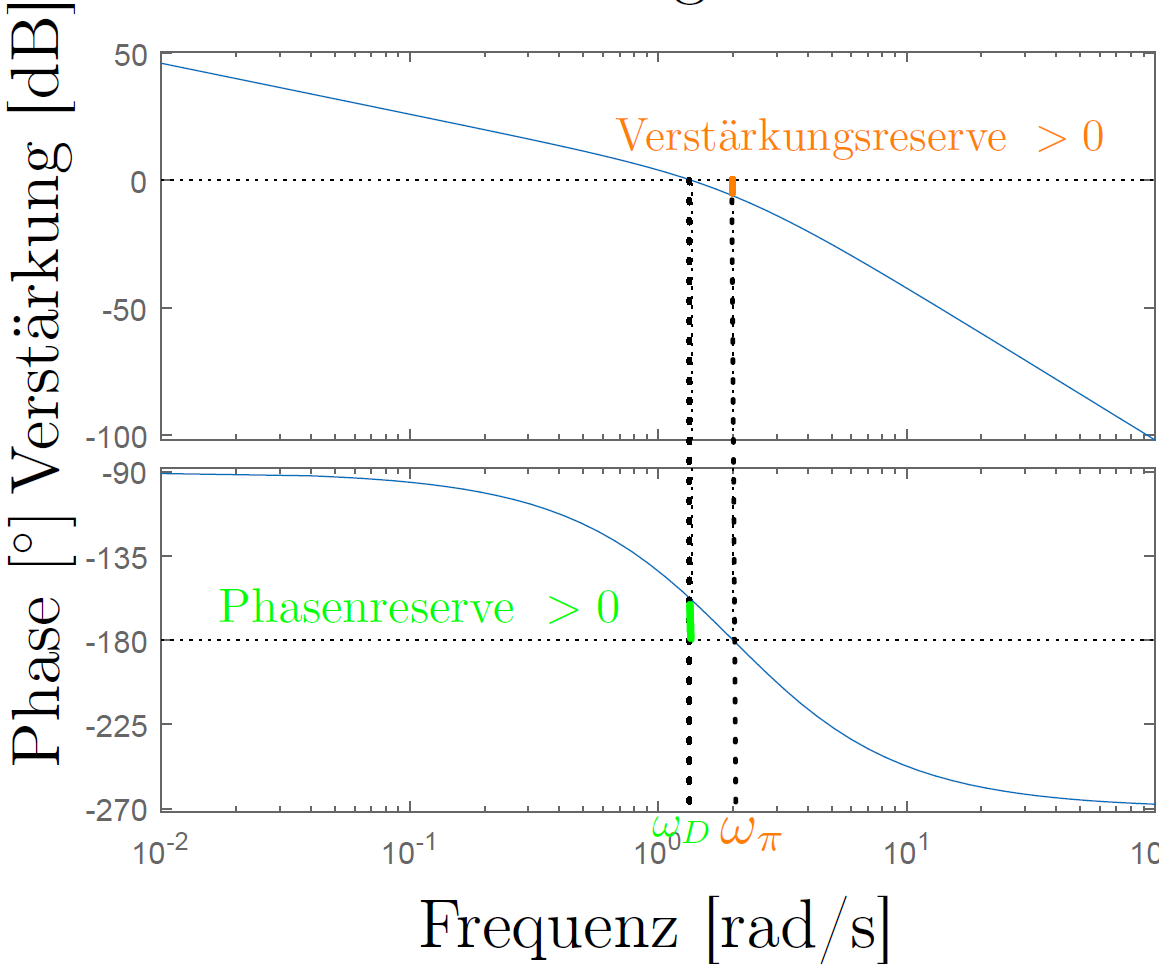
\includegraphics[width=\columnwidth]{images/bodeplot_stabilitaetsreserven.png}
\end{minipage}
\hfill
\begin{minipage}[c]{0.42\columnwidth}
    \begin{itemize}
        \item \cgn{Durchtrittsfrequenz $\omega_{D}$}  %\textrightarrow\ Phasenreserve $\Phi_{RES}$
            $$ K_{RES} = 0 \, \deci \bel - K_{\text{@} 180 \degree } $$ 

        \item \cor{Phasenschnittfrequenz $\omega_{\pi}$} % \textrightarrow\ Verstärkungsreserve $K_{RES}$
            $$ \Phi_{RES} = \Phi_{\text{@}0 \deci \bel }  + 180 \, \degree $$ 
    \end{itemize}
    \crd{\textbf{Achtung:} Das Vorzeichen von $K_{RES}$ bzw. $\Phi_{RES}$ ist essentiell für die Stabilitäts-Beurteilung und
    darf auf keine Fall vernachlässigt werden!}
\end{minipage}


\subsubsection{Beurteilung der Stabilität des Systems}

Wenn das System die \textbf{Anforderungen des Nyquist-Kriteriums erfüllt}, verhält sich die Stabilität des Systems folgendermassen:

\begin{itemize}
    \item \textbf{Grenzstabilität}: Amplitudengang bei $0 \, \deci \bel$ \textbf{und} Phasengang bei $-180 \, \degree$
    \item \textbf{Instabilität}: Amplitudengang $>0 \, \deci \bel$ % CHECK if this is correct
    \item \textbf{Stabilität}: Amplitudengang $<0 \, \deci \bel$ % CHECK
    \item \textbf{Stabilität}: $\omega_{\pi} > \omega_D$  % gemäss Skript
\end{itemize}


\subsection{Bodediagramme mit Matlab}

\lstinputlisting{snippets/bode.m}
        % \section{PID-Regler}

\begin{outline}
    \1 \textbf{P}: Proportional $K_p \cdot e(t)$
        \2 Gegenwart: Gewichtung des \textbf{aktuellen} Fehlers $e(t)$
            \3 Stellgrösse $u(t)$ ist abhängig vom aktuell vorhandenen Fehler
            \3 Wie gross Fehler in Vergangenheit war oder in welche Richtung er sich entwickelt, ist irrelevant
    \1 \textbf{I}: Integral $K_I \int e(t)$
        \2 Vergangenheit: Gewichtung der \textbf{Summe vergangener} Fehler
            \3  Stellgrösse $u(t)$ ist abhängig davon, wie lange ein Fehler schon existiert
            \3 Wie gross der aktuelle Fehler ist und wie start er sich gerade ändert, ist irrelevant
    \1 \textbf{D}: Differential $K_D \cdot \dot{e}(t)$
        \2 Zukunft, Trend: Gewichtung der \textbf{Änderung} des Fehlers
            \3 Stellgrösse ist abhängig davon, wie stark der Fehler gerade zu-/abnimmt
            \3 Wie gros der aktuelle Fehler ist und wie lange er schon existiert, ist irrelevant
\end{outline}


\subsection{Aufbau und Struktur}

\begin{minipage}{0.48\columnwidth}
    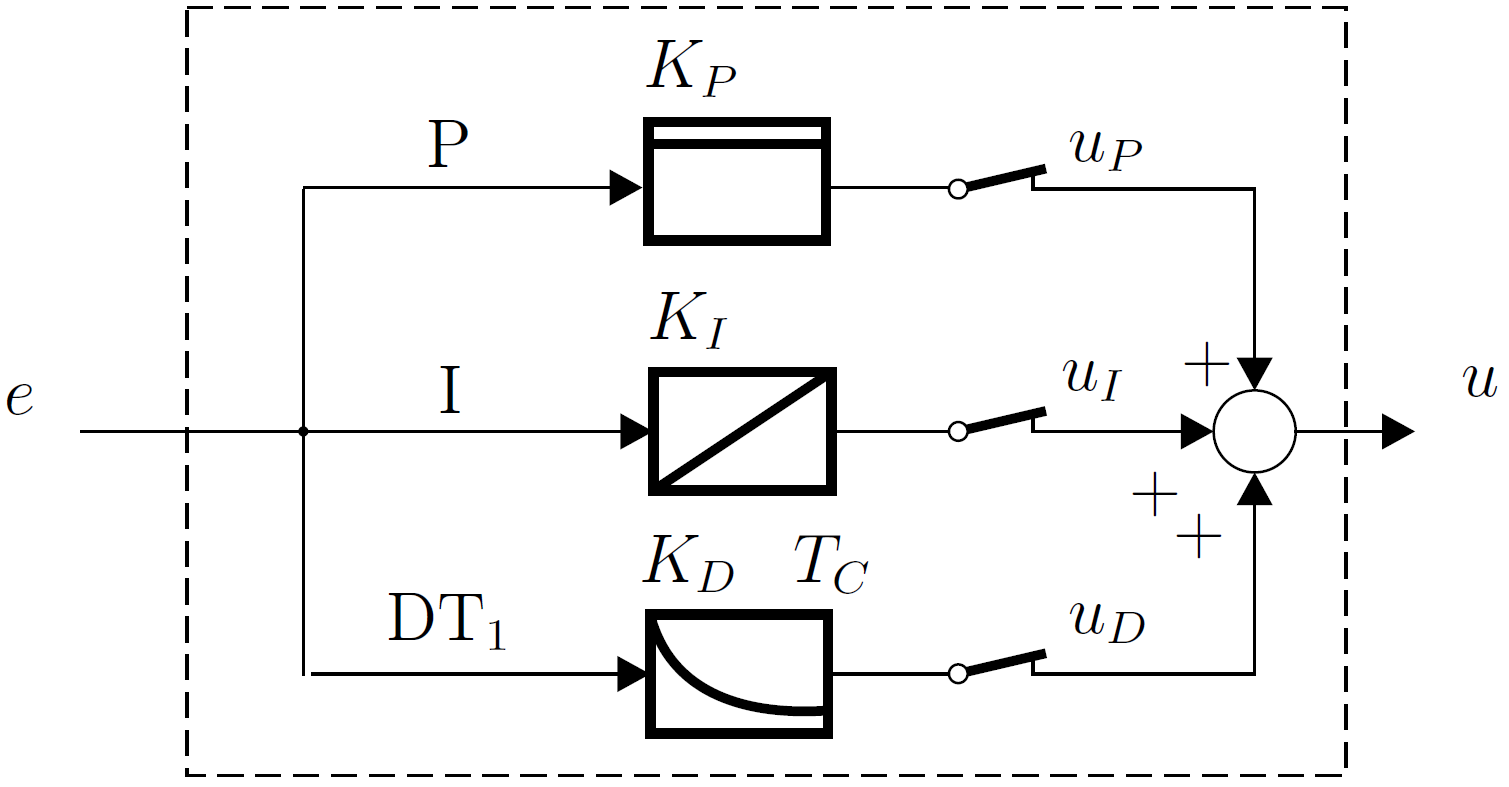
\includegraphics[width=\columnwidth]{images/pid_regler_aufbau.png}
\end{minipage}
\hfill
\begin{minipage}{0.48\columnwidth}
    \begin{center}
        \textbf{Frequenzgang realer PID-Regler}
    \end{center}
    $$ \boxed{ G_{PID}(\jimg \omega) = K_P + \frac{K_I}{\jimg \omega} + K_D \frac{\jimg \omega}{1 + \jimg \omega T_C} } $$
\end{minipage}
        % 
\section{Einstellen eines PID-Reglers} 

\subsection{Vorgehensweisen zum Einstellen eines Reglers}

\begin{minipage}[c]{0.43\columnwidth}
    Regler-Entwuft ist \textbf{iterativer Prozess!}
    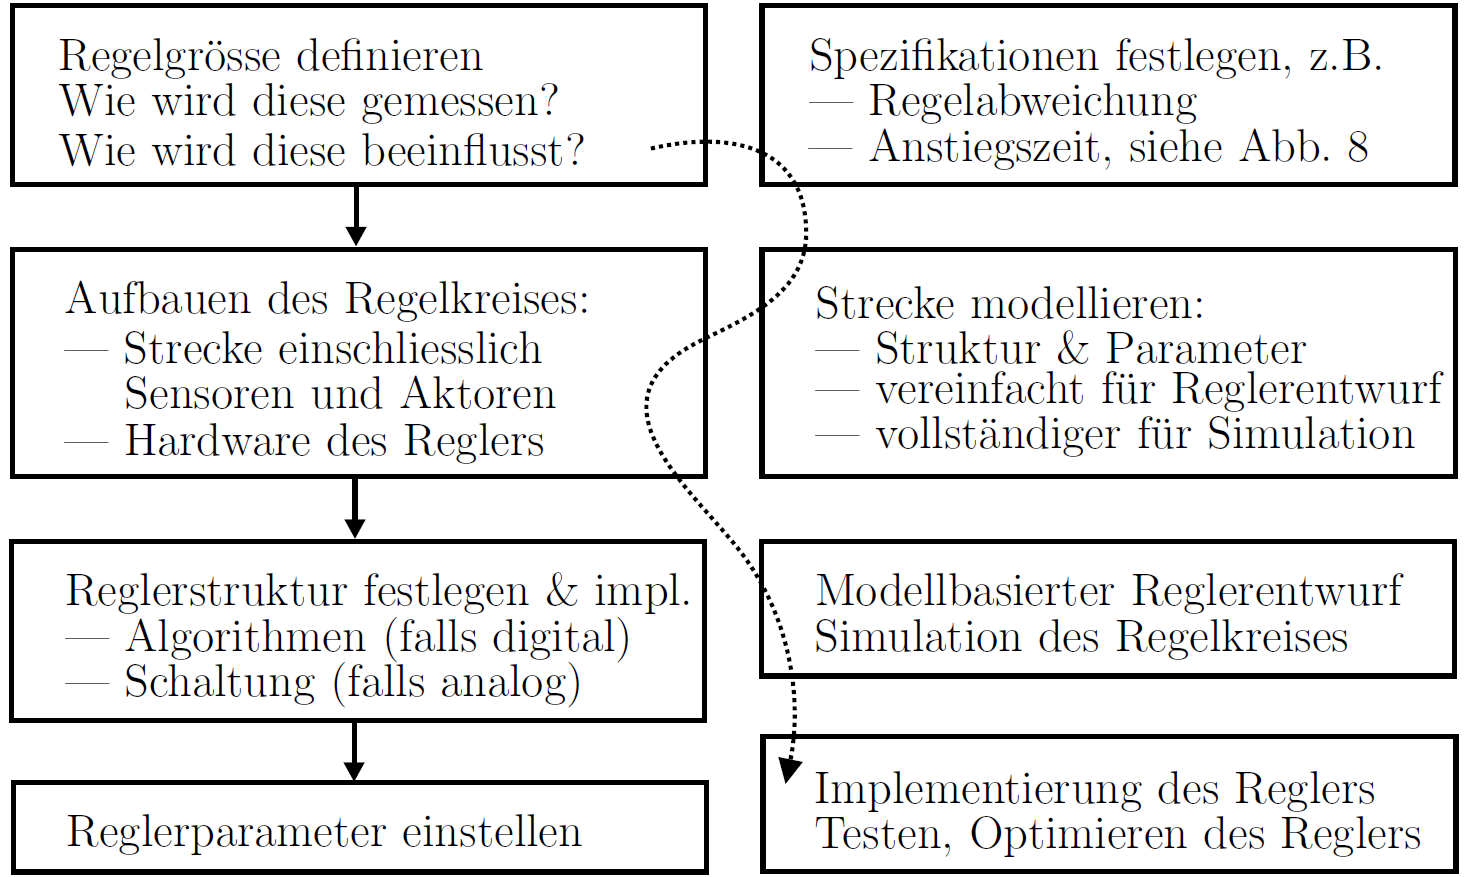
\includegraphics[width=\columnwidth]{images/reglerentwurf_moegliche_schritte.png}
\end{minipage}
\hfill
\begin{minipage}[c]{0.56\columnwidth}
    \begin{outline}
        \1 Experimente an realen Stecken
            \2 Sprungantworten und Frequenzantworten
        \1 Empirische Einstellregeln
            \2 Ziegler/Nichols, Chien/Hrones/Reswick, ...
        \1 Experimente an einem Modell der Strecke
            \2 Simulationen (viele!)
            \2 Sättigung, Rauschen, Unsicherheiten, ...
        \1 Analytischer Entwuft mit einem Modell
            \2 Pol-/Nullstellenkürzung, ...
    \end{outline}
\end{minipage}


\subsubsection{Reale Stecke vs. Modell}

\begin{outline}
    \1 Für einfache Strecken kann komplett auf Modell verzichtet werden
        \2 Zweipunkteregler, P-Regler für Wasserstand
        \2 Trial-and-Error
    \1 Modelle bieten Vorteile
        \2 Strecke ist nicht zugänglich
            \3 Prototyp; nur in kleinen Stückzahlen verfügbar; steht beim Kunden, ...
        \2 Tests dauern lange wegen grosser Zeitkonstante (\textrightarrow\ langes Messen)
        \2 Strecke ist gefährlich (z.B. Atomreaktor)
        \2 Messungen sind schlecht reproduzierbar
\end{outline}


\subsubsection{Analytischer Entwuft vs. Experiment}

\begin{minipage}[t]{0.48\columnwidth}
    \begin{outline}
        \1 Analytischer Entwuft und Analyse mit LZI-Modell
            \2 Sprungantworten (Führungsverhalten, Störverhalten)
            \2 Ortskurven / Bode-Diagramme
            \2 Verstärkungs- und Phasenreserve
            \2 Einfluss von Rauschen
        \1 Simulation mit Nicht-LZI (nichtlinear, zeitvariant)
            \2 Test der Funktionsfähigkeit mit 'genauerem' Modell
            \2 Unterscheidung von Betriebsfällen (Umschaltvorgänge)
                \3 Einschalten, Dauerbetrieb, Fehlerfälle
                \3 Zustandsautomaten
            \2 Wiederholbarkeit gewährleistet
    \end{outline}
\end{minipage}
\hfill
\begin{minipage}[t]{0.48\columnwidth}
    \begin{outline}
        \1 Regler-Tuning mit Experimenten
            \2 Man sieht, spürt und hört den Einfluss des Reglers sofort
                \3 z.B. Vibrationen
            \2 Messungen zur Beurteilung des Reglers (Robustheit) sinnd oft aufwändig
            \2 Experimente können lange dauern und sind oft auch schlecht reproduzierbar
            \2 Man kann sich keien Fehler erlauben!
                \3 Sicherer Betrieb muss gewährleistet sein
    \end{outline}
\end{minipage}


\subsubsection{Kriterien zur Beurteilung des Reglers}

\begin{minipage}[t]{0.48\columnwidth}
    \begin{outline}
        \1 Analytische Modelle
            \2 Pol-Lagen (Zeitkonstanten)
            \2 Frequenzgang (Nyquist, Bode)
            \2 Stabilitätsreserven
            \2 Sprungantworten 
                \3 Überhöhungen, Zeitkonstante
            \2 Gütemasse
    \end{outline}
\end{minipage}
\hfill
\begin{minipage}[t]{0.48\columnwidth}
    \begin{outline}
        \1 Experimente
            \2 Sprungantworten
                \3 Überhöhungen, Zeitkonstante
            \2 Berechnen von Gütemassen 
                \3 z.B. Integration Fehlerquadrat $e(t)^2$ und Stellgrössen $u(t)^2$
            \2 Geräusch-Entwicklung
            \2 Vibrationen
    \end{outline}
\end{minipage}


\subsection{Pol-Nullstellenkürzung}{164}

Hierbei handelt es sich um eine \textbf{analytische} Einstellmetode \textrightarrow\ LZI-Modell der Strecke muss vorliegen!
Der Regler wird dann so entworfen, dass er die \textbf{invertierte Stecke} enthält.
\begin{align*}
    G_R(s) &= \frac{K_R}{s} G_s^{-1}(s) \\
    G_0(s) &= G_R(s) \cdot G_S(s) \frac{K_R}{s} G_s^{-1}(s) \cdot G_S(s) = \frac{K_R}{s} \text{ \textrightarrow\ Integrator} \\
    G_f(s) &= \frac{G_0(s)}{1 + G_0(s)} = \frac{1}{\frac{1}{K_R} s + 1} \text{ \textrightarrow\ PT}_1 \text{-System} 
\end{align*}

\textbf{Hinweis:} Wähle als Reglerstruktur die Standardform (Variante 2) \textrightarrow\ siehe Abschnitt~\ref{PID-Regler Standardform}
\vspace{0.2cm}
Für die Übertragungsfunktionen gelten die folgenden Bezeichnungen:

\begin{minipage}[t]{0.48\columnwidth}
    \begin{tabular}{ll}
    $G_R(s)$    & UTF Regler \\
    $G_S(s)$    & UTF Stecke
\end{tabular}
\end{minipage}
\hfill
\begin{minipage}[t]{0.48\columnwidth}
    \begin{tabular}{ll}
        $G_0(s)$    & UTF offener Regelkreis \\
        $G_f(s)$    & UTF geschlossener Regelkreis  
    \end{tabular}
\end{minipage}


\subsubsection{Eigenschaften der Pol-Nullstellenkürzung}

\begin{outline}
    \1 \textbf{Pol-Nullstellenkürzung darf nur in der linken komplexen Halbebene durchgeführt werden!}
    % \1 Offener Regelkreis $G_0(s)$ wird zu einem Integrator \textrightarrow\ Optimalfall!
    % \1 Geschlossener Regelkreis $G_f(s)$ wird zu einem $\text{PT}_1$-System \textrightarrow\ Optimalfall!
    \1 Das Konzept funktioniert nicht immer
        \2 Inverse $G_s^{-1}(s)$ kann sehr sensitiv auf Modellparameter sein \\
            \textrightarrow\ braucht sehr genaues Modell
        \2 Instabile Stecken
        \2 Stecken mit Verzögerungen bzw. Totzeiten (\textrightarrow\ Regler wird akausal)
\end{outline}


\subsection{Empirische Einstellregeln}

\textbf{Idee:} Anhand weniger Messungen versucht man, über die Stecke genug Informationen zu gewinnen, um einen Regler entwerfen
zu können.


\subsubsection{Einstellung via Schrittantwort}{164-166}

\textbf{Idee:} Eine Stecke wird mit einem Eingangssignal $u(t) = A \cdot \varepsilon(t)$ angeregt und ihre 
Schrittantwort $y(t)$ wird gemessen. An diese gemessene Schrittantwort $y(t)$ wird ein \textbf{$\text{PT}_1$-System mit Totzeit}
'gefittet'. Die daraus entstehenden Parameter werden für die Regler-Dimensionierung verwendet.
$$ \text{PT}_1 \text{-System mit Totzeit} \quad G_0(s) = \frac{K_s}{s \cdot T_g + 1} e^{- s T_u} $$

\begin{minipage}[c]{0.45\columnwidth}
    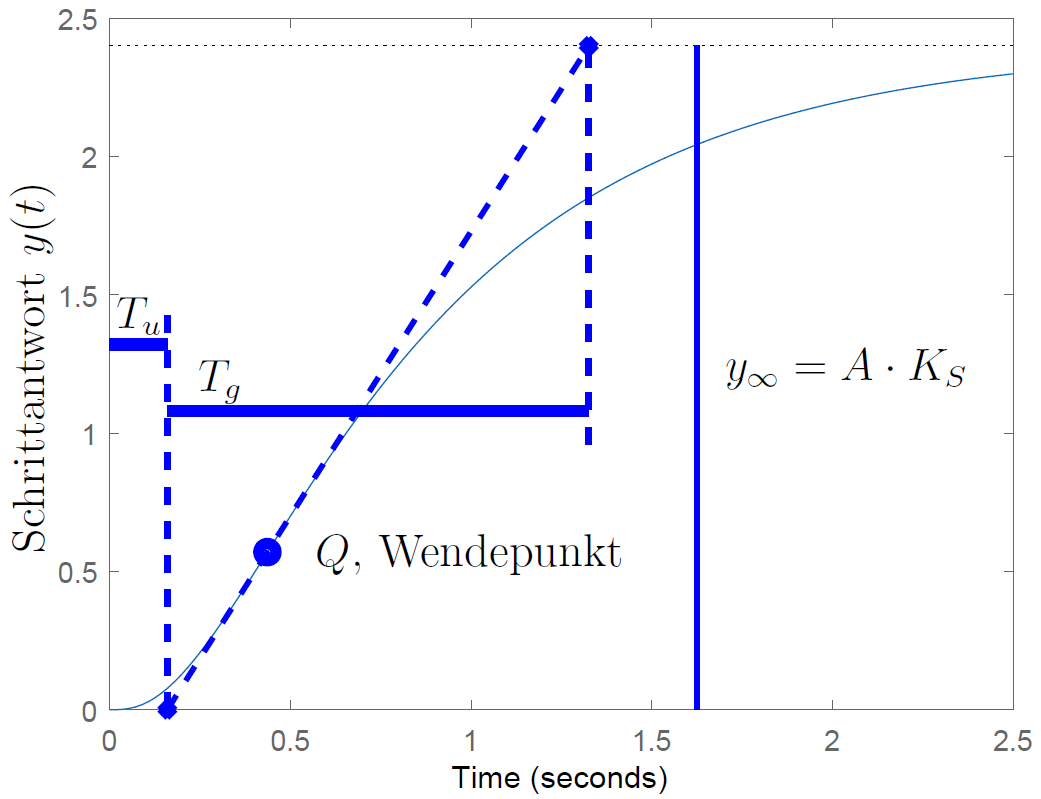
\includegraphics[width=\columnwidth]{images/pid_regler_empirisch_einstellen.png}
\end{minipage}
\hfill
\begin{minipage}[c]{0.52\columnwidth}
    \begin{center}
        \textbf{\myul{Vorgehen $\text{PT}_1$ fitten / Parameter bestimmen}}
    \end{center}

    \begin{outline}
        \1 Tangente an Wendepunkt $Q$ einzeichnen
        \1 Parameter $T_u$, $T_g$ und $K_s$ gemäss Grafik bestimmen
            \2 $K_s$: Verstärkung
            \2 $T_u$: Verzugszeit
            \2 $T_g$: Ausgleichszeit
        \1 Konstanten für Tabellen bestimmen
            \2 $\mu = \frac{T_g}{T_u}$
            \2 $q = \frac{T_g}{T_u \cdot K_s} = \mu \cdot \frac{1}{K_s}$
    \end{outline}
\end{minipage}

\textbf{\myul{Regelbarkeit der Stecke}} \\
Gut regelbar heisst, die Zeitkonstante des geschlossenen Regelkreises ist kleiner als diejenige des offenen Regelkreises.

\begin{itemize}
    \item Gut regelbar: $\mu < 3$
    \item Schlecht regelbar: $\mu > 10$
\end{itemize}

\vspace{0.1cm}

\textbf{ACHTUNG: Struktur der Regler beachten!} Die Tabelle liefert Parameter für Regler in \textbf{serieller Form}
(siehe Abschnitt~\ref{PID-Regler multiplikative Form}) 

\begin{tabular}{c c c }
    $ \boxed{ G_{\rm PID}(s) = K_R \cdot \Bigg( 1 + \frac{1}{s \cdot T_N} + s \cdot T_V \Bigg) }$ & 
    $ \boxed{ G_{\rm PI}(s) = K_R \cdot \Bigg( 1 + \frac{1}{s \cdot T_N} \Bigg) }$ &
    $ \boxed{ G_{\rm P}(s) = K_R }$ 
\end{tabular}

\begin{center}
    \begin{tabular}{|c | c | c | c | c|}
        \toprule
        Regler      & Methode       & $K_R$             & $T_N$                 & $T_V$             \\
        \midrule
                    & ZN            & $1.0 \cdot q$     & $-$                   & $-$               \\
        P-Regler    & CHR (20 \%)   & $0.7 \cdot q$     & $-$                   & $-$               \\
                    & CHR (0 \%)    & $0.3 \cdot q$     & $-$                   & $-$               \\
        \midrule
                    & ZN            & $0.9 \cdot q$     & $3.33 \cdot T_u$      & $-$               \\
        PI-Regler   & CHR (20 \%)   & $0.6 \cdot q$     & $1.0 \cdot T_g$       & $-$               \\
                    & CHR (0 \%)    & $0.35 \cdot q$    & $1.17 \cdot T_g$      & $-$               \\
        \midrule
                    & ZN            & $1.2 \cdot q$     & $2.0 \cdot T_u$       & $0.5 \cdot T_u$   \\
        PID-Regler  & CHR (20 \%)   & $0.6 \cdot q$     & $1.0 \cdot T_g$       & $0.47 \cdot T_u$  \\
                    & CHR (0 \%)    & $0.35 \cdot q$    & $1.17 \cdot T_g$      & $0.5 \cdot T_u$   \\
        \bottomrule
    \end{tabular}
\end{center}

\textbf{Hinweis:} Die Prozentwerte bei CHR beschreiben den Sollwert für Überschwinger.
Zu beachten ist, dass diese Werte durch die empirischen Einstellregeln nicht garantiert werden.


\subsubsection{Einstellung via Stabilitätsgrenze}{166-167}

\textbf{Idee:} Eine stabile Stecke wird mit \textbf{P-Regler} betrieben. Die Verstärkung $K_R$ des Reglers wird sukzessive erhöht,
bis das System \textbf{grenzstabil ist} (endlos mit gleicher Amplitude schwingt).

\begin{minipage}[c]{0.55\columnwidth}
    \begin{tabular}{|c | c | c | c|}
        \toprule
        Regler      & $K_R$                     & $T_N$                 & $T_V$                 \\
        \midrule
        P-Regler    & $0.5 \cdot K_{\rm RES}$   & $-$                   & $-$                   \\
        \midrule
        PI-Regler   & $0.45 \cdot K_{\rm RES}$  & $0.85 \cdot T_{\pi}$  & $-$                   \\
        \midrule
        PID-Regler  & $0.60 \cdot K_{\rm RES}$  & $0.50 \cdot T_{\pi}$  & $0.125 \cdot T_{\pi}$ \\
        \bottomrule
    \end{tabular}
\end{minipage}
\hfill
\begin{minipage}[c]{0.42\columnwidth}
    \begin{center}
        \textbf{\myul{Parameter bestimmen}}
    \end{center}

    \begin{outline}
        \1 Wenn System grenzstabil: Kritisches $K_R$ bestimmen
            \2 $K_{\rm krit} = K_{\rm RES}$
        \1 $T_{\pi}$ Periodendauer der grenzstabilen Schwingung 
    \end{outline}
\end{minipage}

\textbf{ACHTUNG: Struktur der Regler beachten!} Die Tabelle liefert Parameter für Regler in \textbf{serieller Form}
(siehe Abschnitt~\ref{PID-Regler multiplikative Form}) 


\subsection{Regler-Einstellung durch Optimierung}{167}

Im Folgenden ist das Vorgehen zur Regler-Einstellung durch Optimierung beschrieben.

\begin{enumerate}
    \item Reglerstruktur wählen \\
        \textrightarrow\ Regler hat Parameter $k_1, \ldots, k_n$, welche optimiert werden sollen
    \item \textbf{Geschlossenen} Regelkreis (inkl. Strecke) aufbauen (real oder \textbf{Simulation})
    \item Eingangssignale definieren (Führungsgrösse $r(t)$, Störgrösse $z(t)$), für welche Regelkreis optimiert werden soll
        (z.B. Sprung, Rampe)
    \item Gütemass $J$ definieren \textrightarrow\ repräsentative Zahl\\
        Häufig wird $J(k_1, \ldots, k_n) = \int\limits_0^{T_{\rm end}} (k_e \cdot e^2 +k_u \cdot u^2) \diff t$ gewählt
    \item Für verschiedene Parametersätze $k_1, \ldots, k_n$ Signale auf Regelkreis geben und Gütemass $J$ berechnen und beurteilen
        \textrightarrow\ Parameter $k_1, \ldots, k_n$ sind \textbf{optimal}, wenn Gütemass $J$ \textbf{minimal} ist
\end{enumerate}

\textbf{Achtung:} $T_{\rm end}$ sollte minestens so gross sein, dass der Regelkreis bei vernünftiger Reglereinstellung als
eingeschwungen gilt (steady-state).
        % \section{Variationen / Erweiterungen zu PID-Reglern}

\subsection{Modifizierter PID-Regler in Parallelform}{171}

\begin{minipage}[t]{0.4\columnwidth}
    \begin{center}
        \textbf{\myul{Parallelform (normal)}}
    \end{center}
    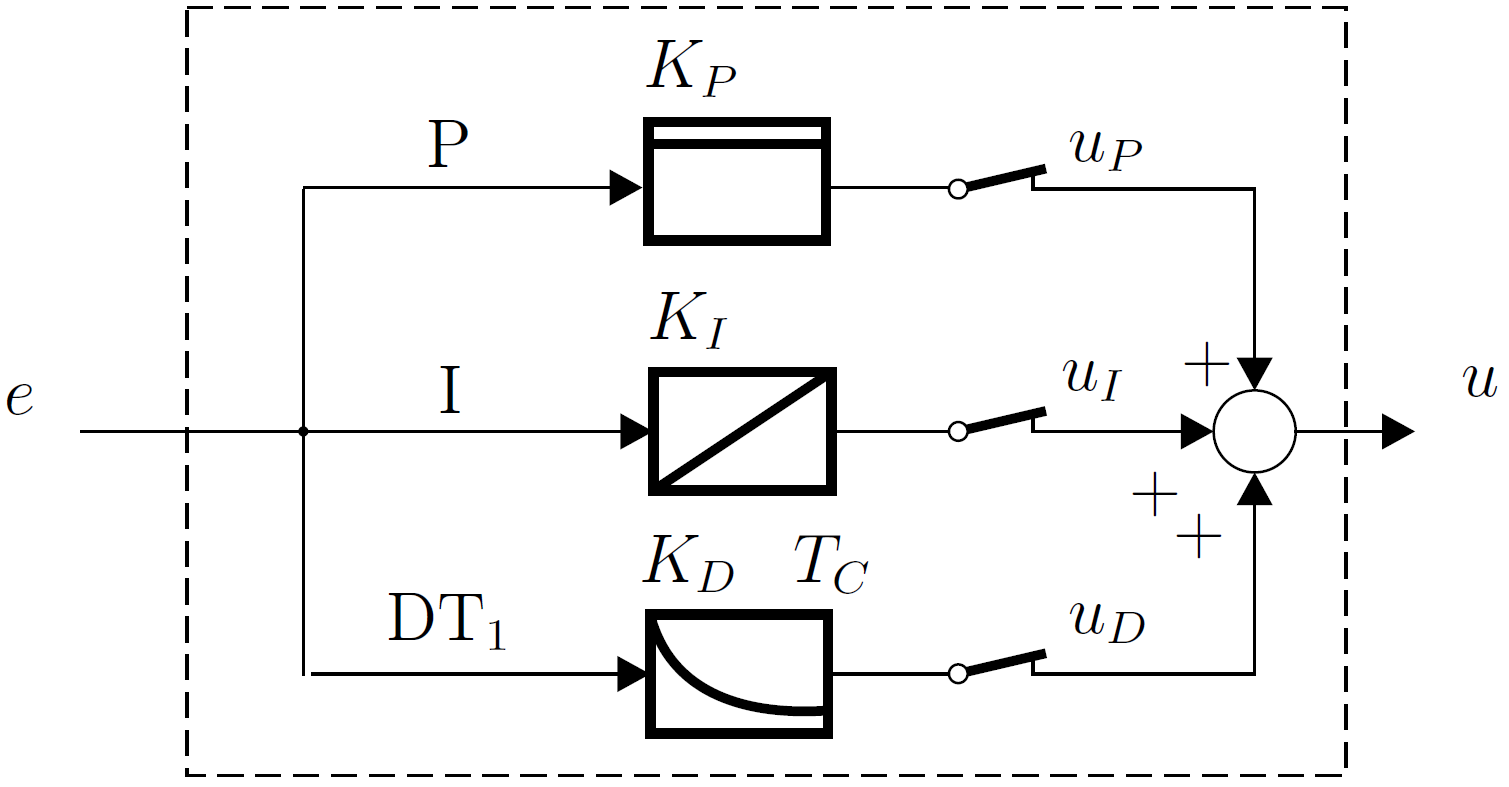
\includegraphics[width=\columnwidth]{images/pid_regler_aufbau.png}

    \textbf{Hinweis:} $P$-Anteil darf auch nach vorne gezogen werden (wie rechts) 
    \textrightarrow\ ändert Parameter von $I$- und $\text{DT}_1$-Gliedern
\end{minipage}
\hfill
\begin{minipage}[t]{0.55\columnwidth}
    \begin{center}
        \textbf{\myul{Modifizierte Form}}
    \end{center}
    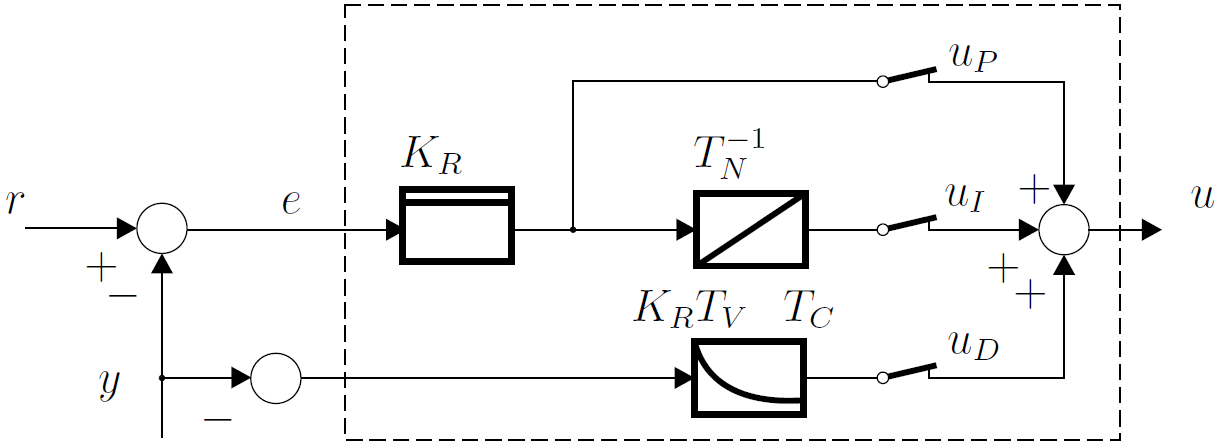
\includegraphics[width=\columnwidth]{images/modifizierter_pid_regler.png}

    Statt Fehler $e$ wird Ausgang $y$ auf $\text{DT}_1$-Glied geführt! \\
    \textrightarrow\ Ableitung des Ausgangs $y$ statt Ableitung des Fehlers $e$
\end{minipage}


\subsubsection{Eigenschaften / Auswirkungen der Modifikation}

\begin{minipage}[t]{0.48\columnwidth}
    \raggedright
    \begin{center}
        \textbf{\myul{Parallelform (normal)}}
    \end{center}

    \begin{outline}
        \1 Ändernde Referenz $r(t)$ (z.B. Sprung)
            \2 $\text{DT}_1$-Glied reagiert sehr aggressiv, da $e(t)$ gross \\
                \textrightarrow\ 'Überforderung' des Stellglieds
    \end{outline}

\end{minipage}
\hfill
\begin{minipage}[t]{0.48\columnwidth}
    \raggedright
    \begin{center}
        \textbf{\myul{Modifizierte Form}}
    \end{center}

    \begin{outline}
        \1 Ändernde Referenz $r(t)$ (z.B. Sprung)
            \2 $\text{DT}_1$-Glied reagiert nicht so aggressiv, da $y(t)$ 'träger' als $e(t)$ \\
                \textrightarrow\  Stellglied 'geschont'
        \1 'two degrees of freedom'
            \2 Reaktion auf Störung bzw. auf Änderung der Referenz separat einstellbar
    \end{outline}
\end{minipage}

\textbf{Achtung:} Der $\text{DT}_1$-Anteil kann nicht einfach weggelassen werden! 


\subsection{Glättung der Referenz}{171}

\begin{minipage}[c]{0.38\columnwidth}
    % 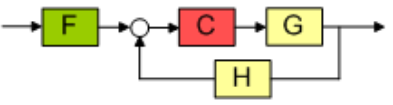
\includegraphics[width=\columnwidth]{images/filterung_stellgroesse.png}
    \begin{center}
    \scalebox{0.4}{
    \begin{tikzpicture}
        [
            scale = 1,
            >=latex,
            orangebox/.style={rectangle, draw=black, fill=orange, thick, minimum width=1cm, minimum height=0.5cm},
            greenbox/.style={rectangle, draw=black, fill=green, thick, minimum width=1cm, minimum height=0.5cm},
            yellowbox/.style={rectangle, draw=black, fill=yellow, thick, minimum width=1cm, minimum height=0.5cm},
            whitecircle/.style={circle, draw=black, fill=white, thick, inner sep=0pt,minimum size=0.3cm},
        ]

        % nodes
        \node               (R)                                     {$r(t)$};
        \node[greenbox]     (F)       [right= of R]                 {F};
        \node[whitecircle]  (A)       [right= of F]                 {};
        \node[orangebox]    (C)       [right= of A]                 {C};   
        \node[yellowbox]    (G)       [right= of C]                 {G};
        \node[yellowbox]    (H)       [below left= of G]            {H};
        \node               (U)       [right= of G]                 {$u(t)$};

        % arrows
        \draw[->, thick]    (R)         to (F.west);
        \draw[->, thick]    (F.east)    to (A.west);
        \draw[->, thick]    (A.east)    to (C.west);
        \draw[->, thick]    (C.east)    to (G.west);
        \draw[->, thick]    (G.east) -> node {} coordinate(U-G) (U);
        \draw[->, thick]    (U-G)       to (H.east);
        \draw[->, thick]    (H.west)    to (A.south);        
    \end{tikzpicture}}
\end{center}
 
\end{minipage}
\hfill
\begin{minipage}[c]{0.6\columnwidth}
    Die Stellgrösse $r(t)$ wird geglättet, um die Spitzenbelastung für das Stellglied zu mindern. Die wird erreicht, indem die 
    Stellgrösse mittels (\cgn{Filter F}) gefiltert wird. \textrightarrow\ Stellglied wird nicht überstrapaziert.
\end{minipage}


\subsection{Störgrössenaufschaltung}{174}

\begin{minipage}[c]{0.55\columnwidth}
    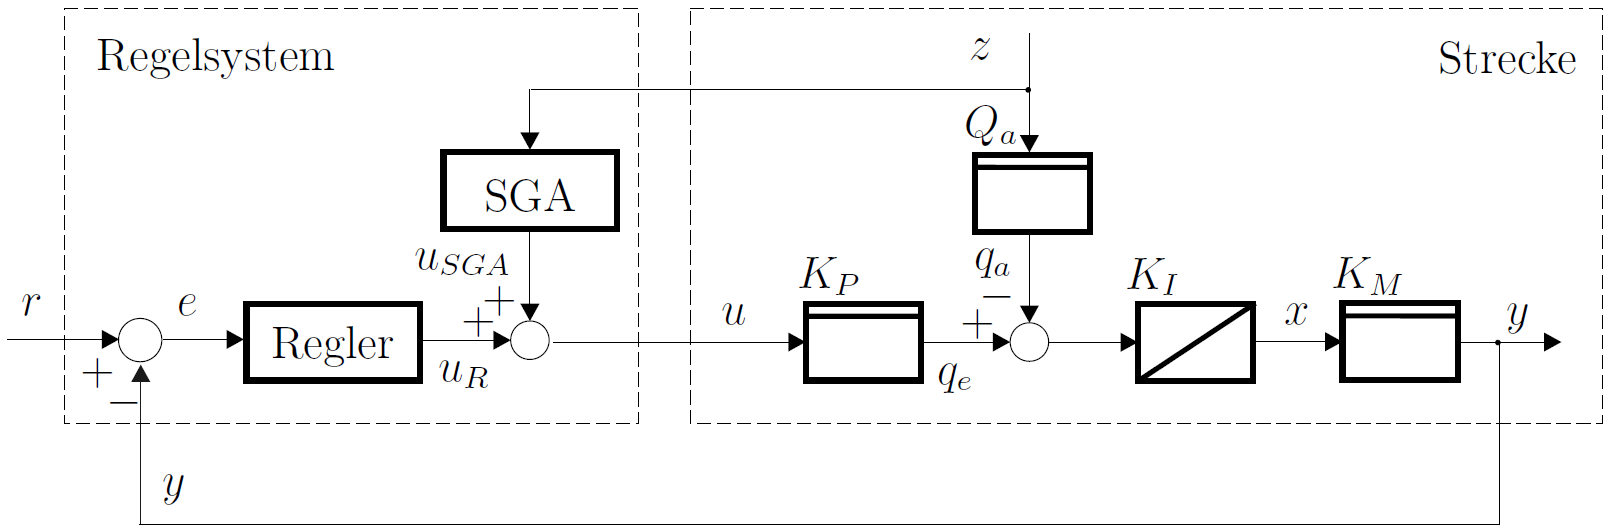
\includegraphics[width=\columnwidth]{images/stoergroessenaufschaltung.png}
\end{minipage}
\hfill
\begin{minipage}[c]{0.43\columnwidth}
    Durch Messungen wird versucht, den Einfluss von Störungen $z(t)$ auf die Strecke gleich im Vornherein mittels 
    \cbl{SGA} zu kompensieren.
\end{minipage}

\vspace{0.2cm}

\begin{minipage}[t]{0.48\columnwidth}
    Am \cgn{grünen Knoten} gilt:
    $$ \dot{y} = K_M K_I [K_P u(t) - Q_a z(t)] $$
    Die Störung soll mittels \textbf{additiver Korrektur} des Reglerausgangs $u_R(t)$ erfolgen. 

    Aus dem Blockschaltbild ersichtlich:
    $$u(t) = u_R(t) + u_{\rm SGA}(t) $$

    $u_{\rm SGA}(t)$ soll den Einfluss von $z(t)$ am \cbl{blauen Knoten} kompensieren.
\end{minipage}
\hfill
\begin{minipage}[t]{0.48\columnwidth}
    Am \cbl{blauen Knoten} gilt:
    $$ \dot{y} = K_M K_I [K_P u_R(t) + \underbrace{ K_p u_{\rm SGA}(t) - Q_a z(t)}_{\text{soll sich auslöschen}}] $$
    Wähle $u_{\rm SGA}(t)$ so, dass die gewünschte Auslöschung stattfindet:
    $$ u_{\rm SGA}(t) = \frac{Q_a}{K_P} z(t) $$
    Somit wird die Störung kompensiert und es bleibt:
    $$ \dot{y} = K_M K_I K_P u_R(t)$$
\end{minipage}


\subsection{Kaskadenregelung}{175}

Regelstrecken 1. und 2. Ordnung ($\text{PT}_1$, $\text{PT}_2$, $I$, $\text{IT}_1$) können gut mit PID-Reglern gereglet werden. 
Bei Strecken höherer Ordnung liefert dieses Vorgehen keine genügenden Resultate mehr.

\begin{itemize}
    \item Geschlossener Regelkreis ist zu lange oder zu wenig gedämpft
    \item Einstellregeln funktionieren gar nicht, weil die Regelstrecke im offenen Betrieb immer instabil ist
\end{itemize}

\textbf{Konsequenz:} Für Strecken höherer Ordnung braucht es auch einen Regler höherer Ordnung \textrightarrow Kaskadenregelung


\subsection{Übertragungsfunktionen Kaskadenregelung}

\begin{minipage}[c]{0.56\columnwidth}
    % 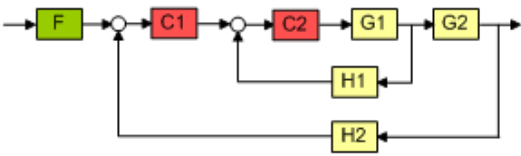
\includegraphics[width=\columnwidth]{images/kaskadenregelung_struktur.png}
    \begin{center}
    \scalebox{0.63}{
    \begin{tikzpicture}
        [%
            scale = 1,
            >={Latex[length=1.5mm]},
            every node/.style={%
                font=\footnotesize, 
                rectangle, 
                draw, 
                minimum width=6mm, 
                minimum height=4mm
            },
            clearnode/.style={%
                rectangle, 
                draw=none, 
                fill=none, 
                minimum width=5mm, 
                minimum height=5mm, 
                inner sep=0pt
            },
            whitecircle/.style={%
                circle, 
                draw=black, 
                fill=white, 
                inner sep=0pt,
                minimum size=2mm
            },
        ]

        % nodes
        \node[clearnode]    (R)                         {$r(t)$};
        \node[fill=green]   (F)     [right=5mm of R]       {F};
        \node[whitecircle]  (A1)    [right=5mm of F]       {};
        \node[fill=orange]  (C1)    [right=5mm of A1]      {C1};   
        \node[whitecircle]  (A2)    [right=5mm of C1]      {};
        \node[fill=orange]  (C2)    [right=5mm of A2]      {C2};   
        \node[fill=yellow]  (G1)    [right=5mm of C2]      {G1};
        \node[fill=yellow]  (G2)    [right=5mm of G1]      {G2};
        \node[fill=yellow]  (H1)    [below=3mm of {$(A2.south west)!0.5!(G1.south east)$}] {H1};
        \node[fill=yellow]  (H2)    [below=3mm of H1]      {H2};
        \node[clearnode]    (U)     [right=5mm of G2]      {$u(t)$};

        % arrows
        \begin{scope}[every path/.style={->, thick}]
            \coordinate (G1G2) at ($(G1.east)!0.4!(G2.west)$);
            \coordinate (G2U) at ($(G2.east)!0.4!(U.west)$);
            
            \draw   (R)         to (F.west);
            \draw   (F.east)    to (A1.west);
            \draw   (A1.east)   to (C1.west);
            \draw   (C1.east)   to (A2.west);
            \draw   (A2.east)   to (C2.west);
            \draw   (C2.east)   to (G1.west);
            \draw   (G1.east)   to (G2.west);
            \draw   (G2.east)   to (U);
            \draw   (G1G2)      to (G1G2|-H1.east) to (H1.east); 
            \draw   (G2U)       to (G2U|-H2.east) to (H2.east); 
            \draw   (H2.west)   to (H2.west-|A1.south) to (A1.south);
            \draw   (H1.west)   to (H1.west-|A2.south) to (A2.south);
        \end{scope}
    \end{tikzpicture}}
\end{center}
    $$ \text{Annahme - Ideale Sensoren: } H_1 = H_2 = 1$$
    
\end{minipage}
\hfill
\begin{minipage}[c]{0.43\columnwidth}
    UTF innerer Regelkreis
    $$ G_{f1} = \frac{G_1 C_2}{1 + G_1 C_2} $$
    UTF äusserer Regelkreis
    $$ \textstyle{ G_{f2} = \frac{G_2 G_{f1} C_1}{1 + G_2 G_{f1} C_1} = \frac{G_2 G_1 C_2 C_1}{1 + G_1 C_2 + G_2 G_1 C_2 C_2}} $$
\end{minipage}

\vspace{0.2cm}
\textbf{Der innere Regelkreis ist deutlich schneller als der äussere Regelkreis!}

$$ G_{f1} \approx K_1 \Rightarrow G_{f2} \approx \frac{G_2 K_1 C_1}{1 + G_2 K_1 C_1} = \frac{G_3 C_1}{1 + G_3 C_1} \Rightarrow G_3 = G_2 K_1 $$

$$ G_{f1} \approx 1  \Rightarrow G_{f2} \approx \frac{G_2 C_1}{1 + G_2 C_1}  $$

\textbf{Interpretation:} Der äussere Regelkreis sieht den inneren Regelkreis nur als Verstärkung $K_1$. Wird $K_1 = 1$ gesetzt, so
ist der innere Regelkreis aus sicht des äusseren Regelkreises gar nicht vorhanden.


\subsubsection{Eigenschaften der Kaskadenregelung}

\begin{outline}
    \1 Der innere Regelkreis muss \textbf{deutlich schneller} sein, als der äussere Regelkreis
        \2 Innere Regelkreis erscheint somit für äusseren Regelkreis nur als eine \textbf{Konstante}
    \1 Der innere Regelkreis wird \textbf{zuerst} ausgelegt
        \2 Dynamik der inneren Regelstrecke verbessern (schneller machen)
        \2 Allenfalls ist eine gute Störunterdrückung wichtig ($G_z(s) = \frac{Z(s)}{Y_{\rm sub}(s)}$ optimieren)
    \1 Beide Regelkreise können mit \textbf{Einstellregeln} eingestellt werden
        \2 Innerer Regelkreis: Äusseren Regelkreis als offen ('nicht da') betrachten
        \2 Äusserer Regelkreis: Innerer Regelkreis muss geschlossen sein (und funktionieren)
    \1 Verfahren ist erweiterbar auf mehrstufige Kaskaden
\end{outline}


\example{Drehzahlregelung Elektromotor mit Kaskadenregelung}

\begin{minipage}[c]{0.5\columnwidth}
    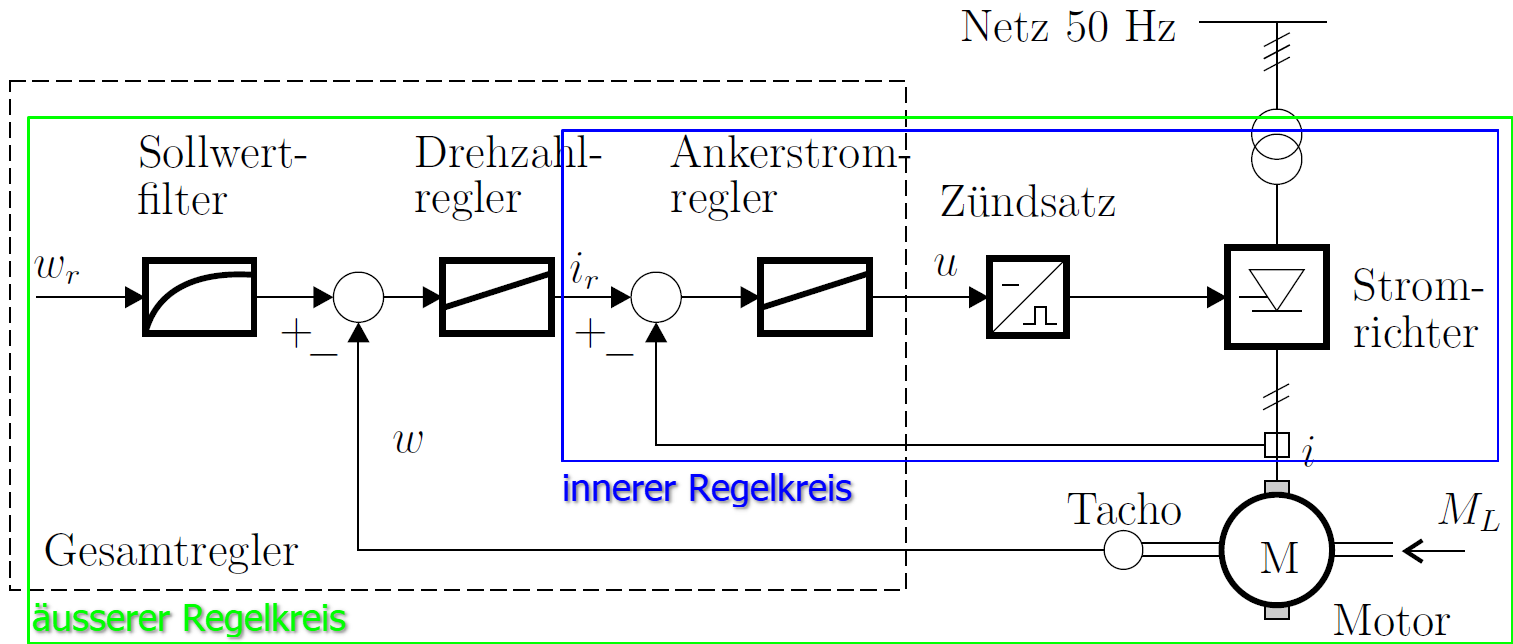
\includegraphics[width=\columnwidth]{images/kaskadenregelung_beispiel.png}
\end{minipage}
\hfill
\begin{minipage}[c]{0.48\columnwidth}
    \begin{outline}
        \1 Der innere Regelkreis regelt den Strom
            \2 Regelgrösse $r_1(t)$: Strom
            \2 Stellgrösse $u_1(t)$: Spannung
        \1 Der äussere Regler regelt die Drehzahl
        \2 Regelgrösse $r(t)$: Drehzahl
        \2 Stellgrösse $u(t) = r_1(t)$: Strom
    \end{outline}
\end{minipage}


\subsection{Wind-Up (Integratoren)}{172}

Das Wind-Up Problem tritt auf, die folgenden drei Voraussetungen erfüllt sind

\begin{itemize}
    \item Der Regler enthält einen \textbf{I-Anteil}
    \item Der Regelkreis enthält eine Limitierung bzw. \textbf{Sättigung} (Stellglied, Sensor, Physik)
    \item Das \textbf{Reglersignal} läuft in die \textbf{Sättigung}
\end{itemize}

\vspace{0.2cm}
Solange der Regelkreis in Sättigung ist

\begin{itemize}
    \item Ausgang der Sättigung ist \textbf{konstant} (und somit auch der Fehler $e(t)$)
    \item Regelkreis verhält sich, als ob der Regelkreis an der Stelle der Sättigung geöffnet wurde
    \item Intergrator im Regelkreis wird zum offenen Integrator und \textbf{'läuft davon'}, da ein konstanter Fehler $e(t)$ ungebremst
        integriert wird \textrightarrow\ Wind-Up
\end{itemize}

\vspace{0.2cm}
Sobald der Wert der Stellgrösse $r(t)$ ändert und der Fehler $e(t)$ umgekehrtes Vorzeichen bekommt, muss erst einmal einige Zeit
abintegriert werden, bis der Regler auf die Änderung der Stellgrösse reagiert. \textrightarrow\ siehe Beispiel


\example{Wind-Up mit PI-Regler}

\begin{minipage}[c]{0.48\columnwidth}
    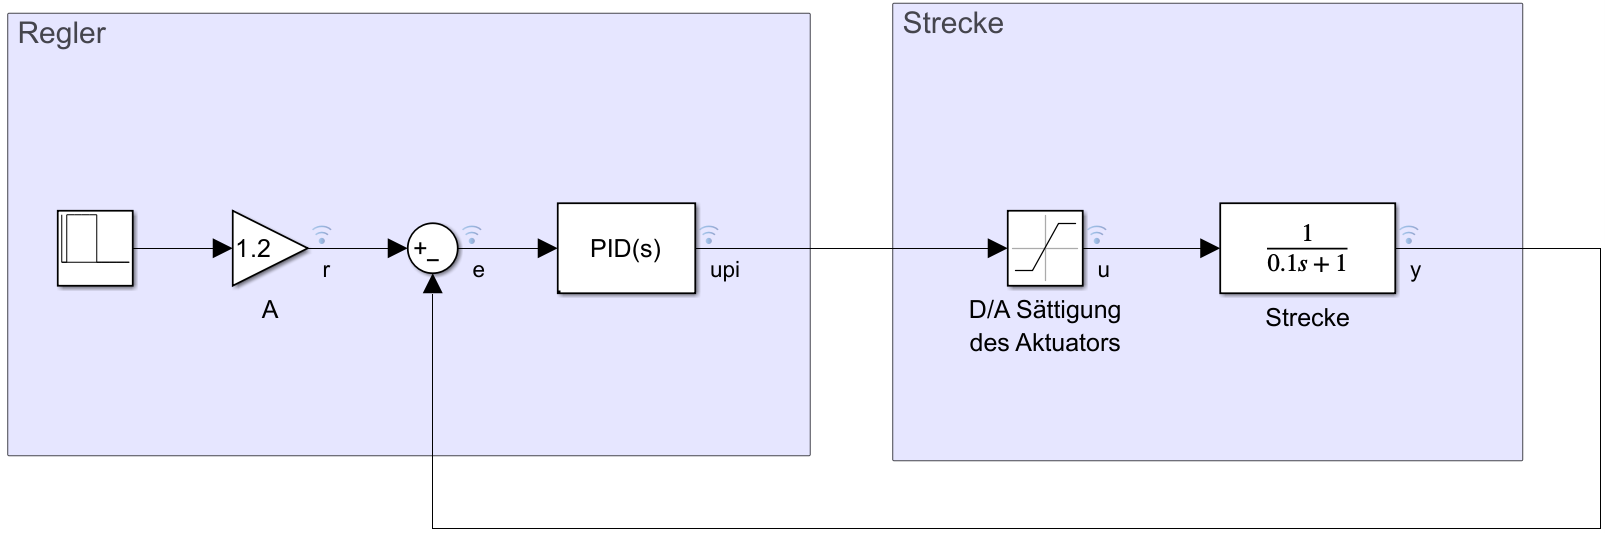
\includegraphics[width=\columnwidth]{images/windup_beispiel.png}
\end{minipage}
\hfill
\begin{minipage}[c]{0.48\columnwidth}
    \begin{itemize}
        \item PI-Regler (so dimensioniert, dass $G_0$ nur noch I-Verhalten hat) \\
            \textrightarrow\ $G_f$ hat $\text{PT}_1$-Verhalten
        \item Sättigungsblock: Sättigung bei $\pm 1$
        \item Stellgrösse $r(t) = 1$ (keine Sättigung)
        \item Stellgrösse $r(t) = 1.2$ (Sättigung)
    \end{itemize}
\end{minipage}

\vspace{0.2cm}
\begin{minipage}[c]{0.4\columnwidth}
    \begin{center}
        \myul{Keine Sättigung (kein Wind-Up)}
    \end{center}
    \vspace{-0.2cm}
    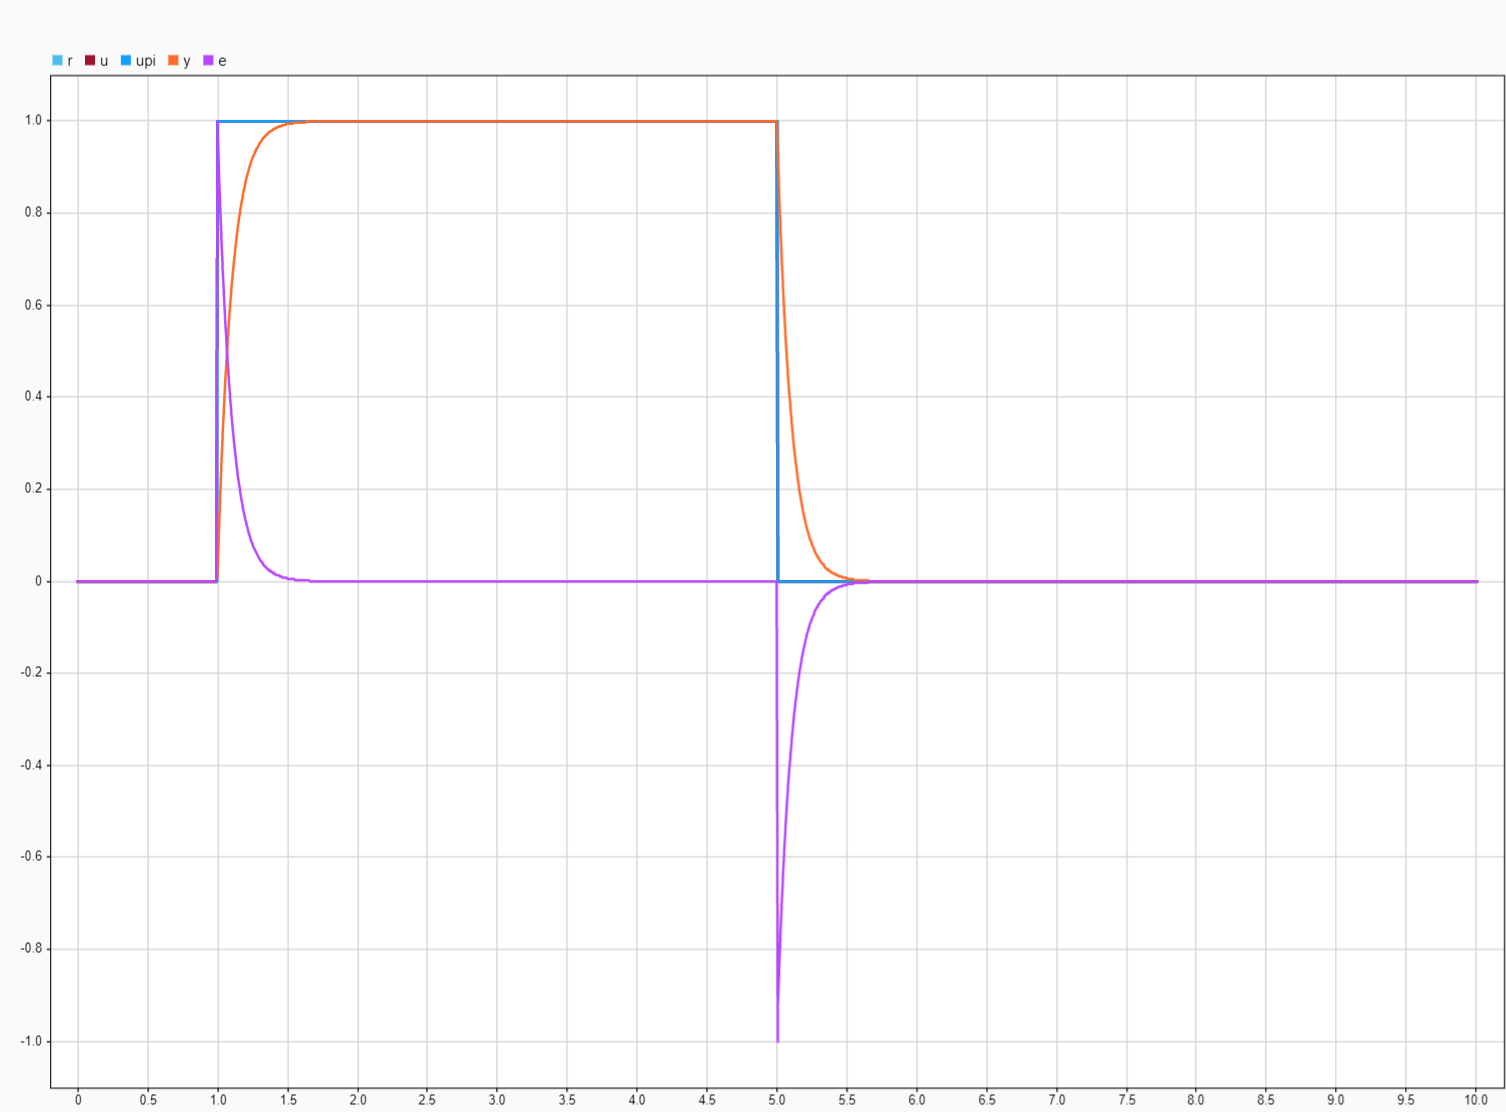
\includegraphics[width=\columnwidth]{images/windup_beispiel_plot_normal.png}
\end{minipage}
\hfill
\begin{minipage}[c]{0.4\columnwidth}
    \begin{center}
        \myul{Sättigung (Wind-Up)}
    \end{center}
    \vspace{-0.2cm}
    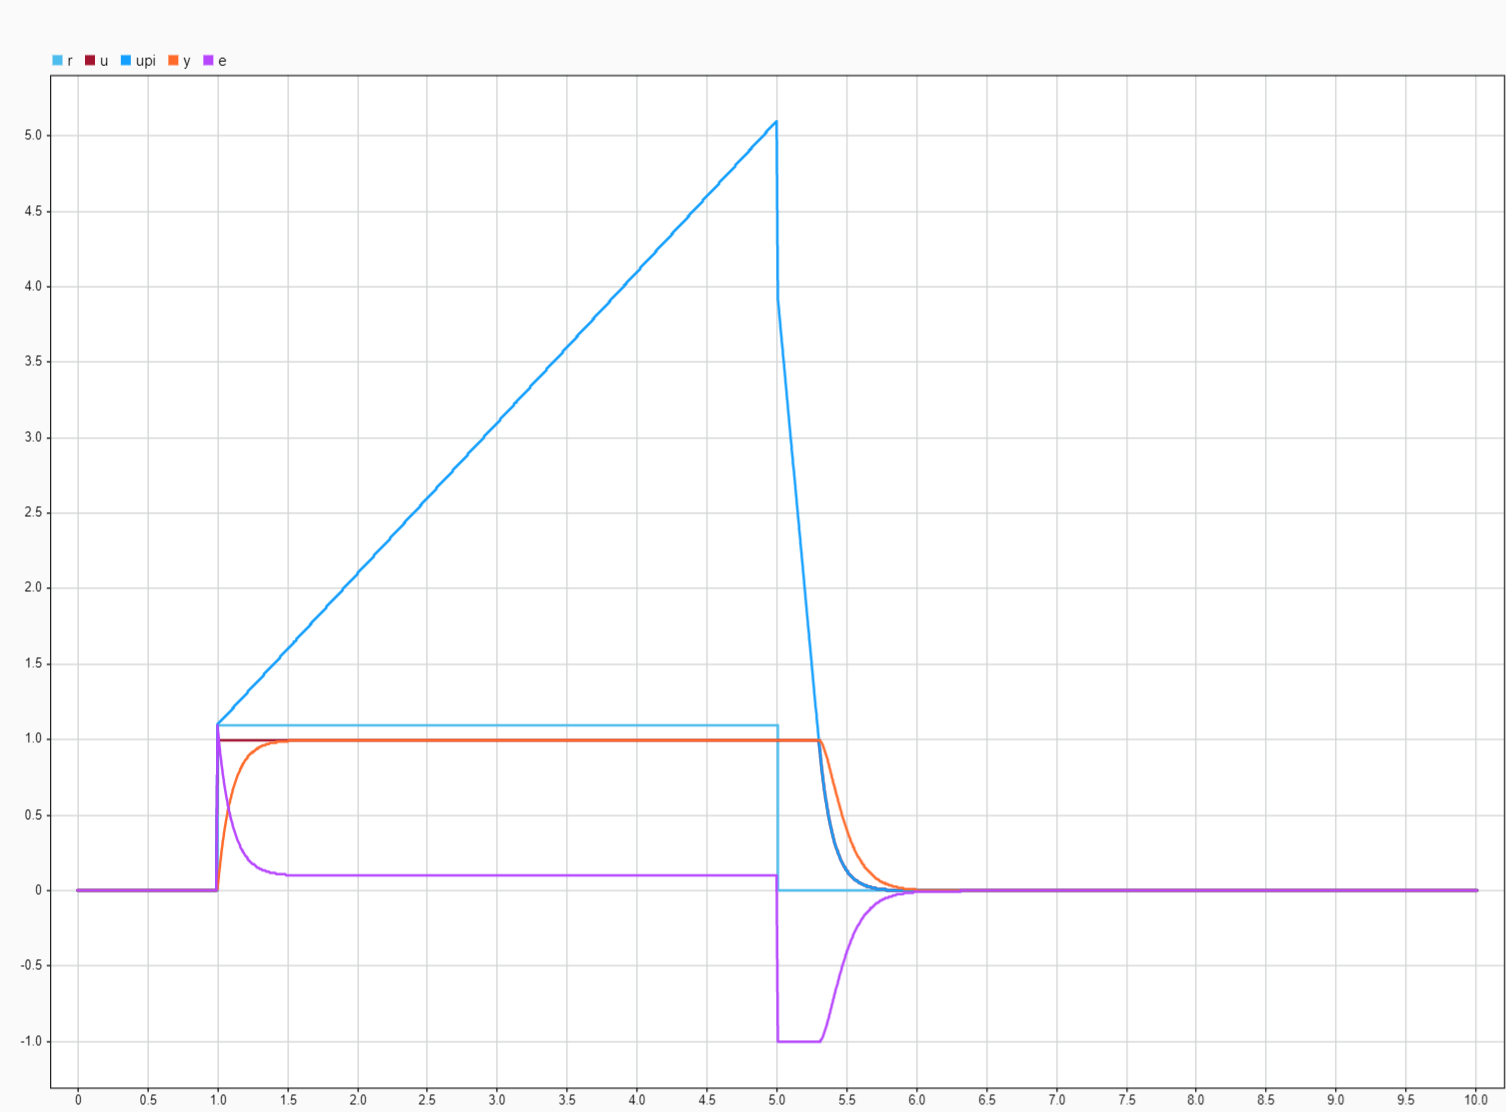
\includegraphics[width=\columnwidth]{images/windup_beispiel_plot_windup_effekt.png}
\end{minipage}


\subsubsection{Anti-Wind-Up-Ansätze}

\textbf{Hinweis:} Die beschriebenen Methoden sind nicht mathematisch, sondern werden durch Simulationen / Ausprobieren umgesetzt.

\begin{itemize}
    \item Wind-Up detektieren und Integrator nach Wind-Up auf \textbf{sinnvollen Wert} setzen
    \item Integrator begrenzen (z.B. auf $80 \, \%$ der möglichen Stellgrösse) \textrightarrow\ nie 'vollgas'
    \item Bedingte Integration (Clamping): Integration stoppen (z.B. wenn Aktor am Limit ist)
\end{itemize}


\begin{minipage}[c]{0.48\columnwidth}
    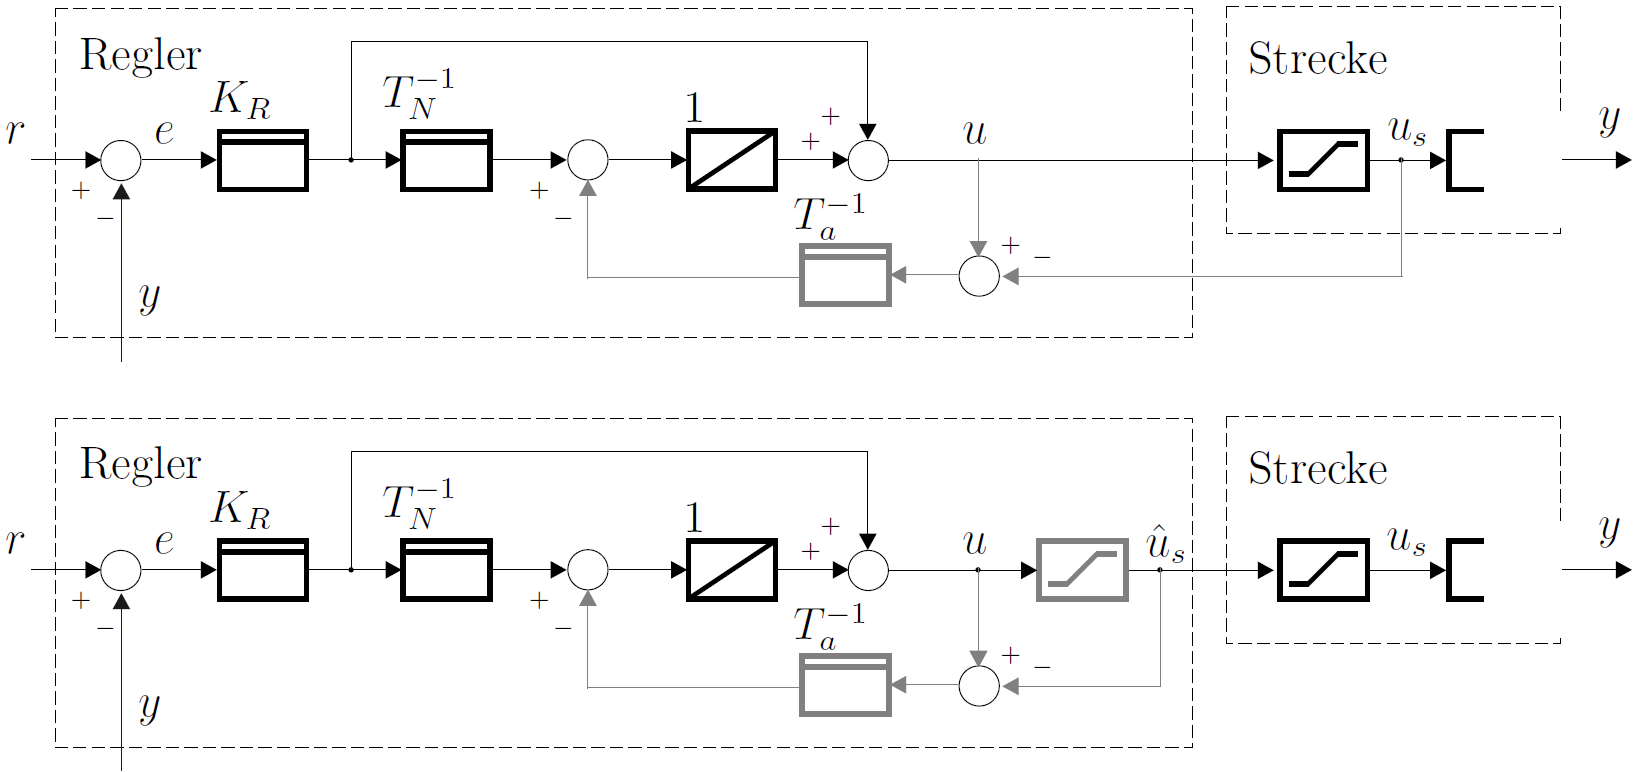
\includegraphics[width=\columnwidth]{images/anti-wind-up.png}
\end{minipage}
\hfill
\begin{minipage}[c]{0.48\columnwidth}
    \begin{itemize}
        \item Feedback-Mechanismus\\
            (\textbf{Back-Calculation})
    \end{itemize}
    \vspace{0.2cm}

    \textrightarrow\ Muss richtig dimensioniert sein! \\
    \textrightarrow\ PI-Regler: Wähle $T_a \approx T_N$
\end{minipage}

\textbf{Achtung: Es braucht immer ein Anti-Wind-Up}, ansonsten läuft der Prozess schlecht oder geht sogar kaputt.


        % \section{Fallstudie: Gleichstromantrieb}

\subsection{Modellierung}{53}
\begin{center}
    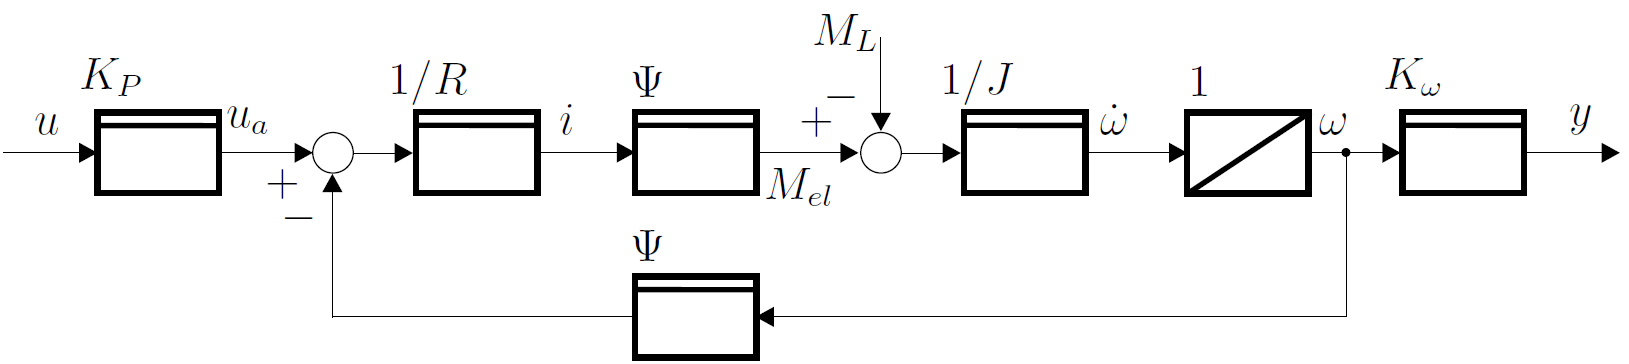
\includegraphics[width=0.75\columnwidth]{images/vereinfachtes_modell_gleichstromantrieb.png} 
\end{center}
Der Gleichstromantrieb kann als $\text{PT}_1$-Glied mit zwei Eingängen $u(t)$ und $M_L(t)$ modelliert werden. $M_L(t)$ entspricht
einer durch Wirbelströme erzeugte \textbf{Störung}.
$$ \boxed{ \underbrace{\frac{R \cdot J}{\Psi^2}}_{T} \dot{y}(t) + y(t) = \underbrace{\frac{K_P \cdot K_{\omega}}{\Psi}}_{K_1} u(t)
    - \underbrace{\frac{R \cdot K_{\omega}}{\Psi^2}}_{K_2} M_L(t) } $$


\subsubsection{Parameter-Identifikation}

\begin{minipage}[c]{0.48\columnwidth}
    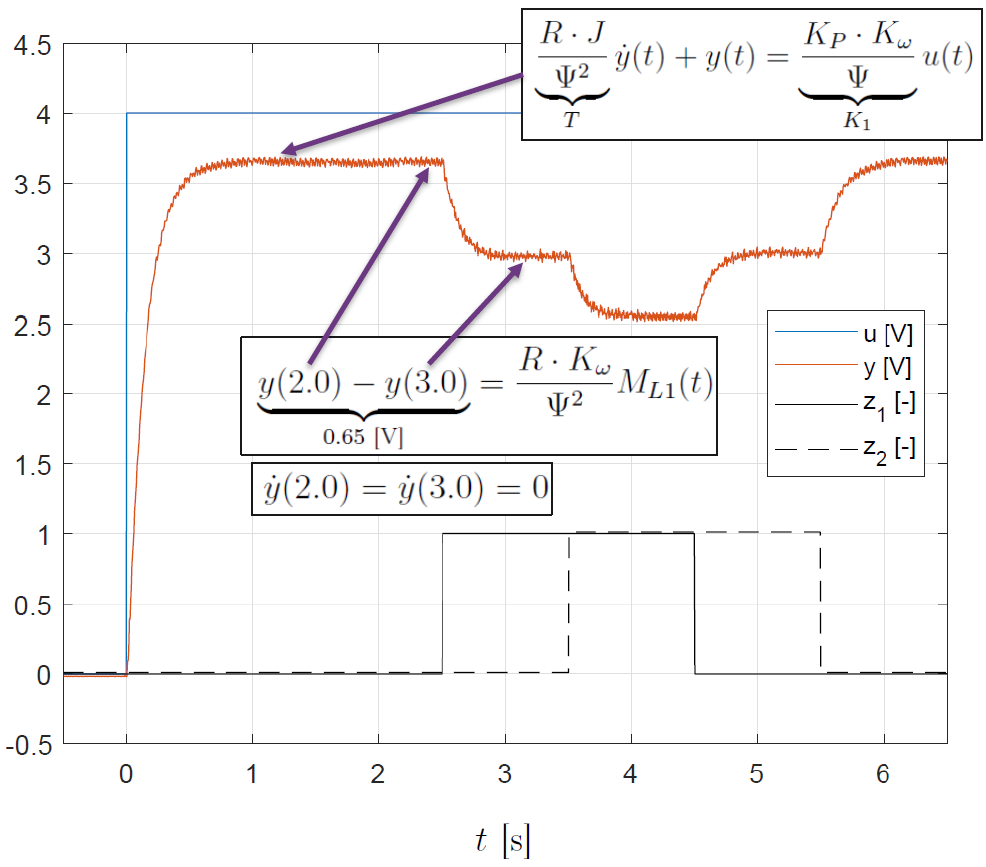
\includegraphics[width=\columnwidth]{images/gleichstrommodell_parameteridentifikation.png}
\end{minipage}
\hfill
\begin{minipage}[c]{0.48\columnwidth}
    Aus der \textbf{Sprungantwort} können einige Parameter abgelesen werden. Einige weitere Parameter sind aus Datenblättern bekannt.
    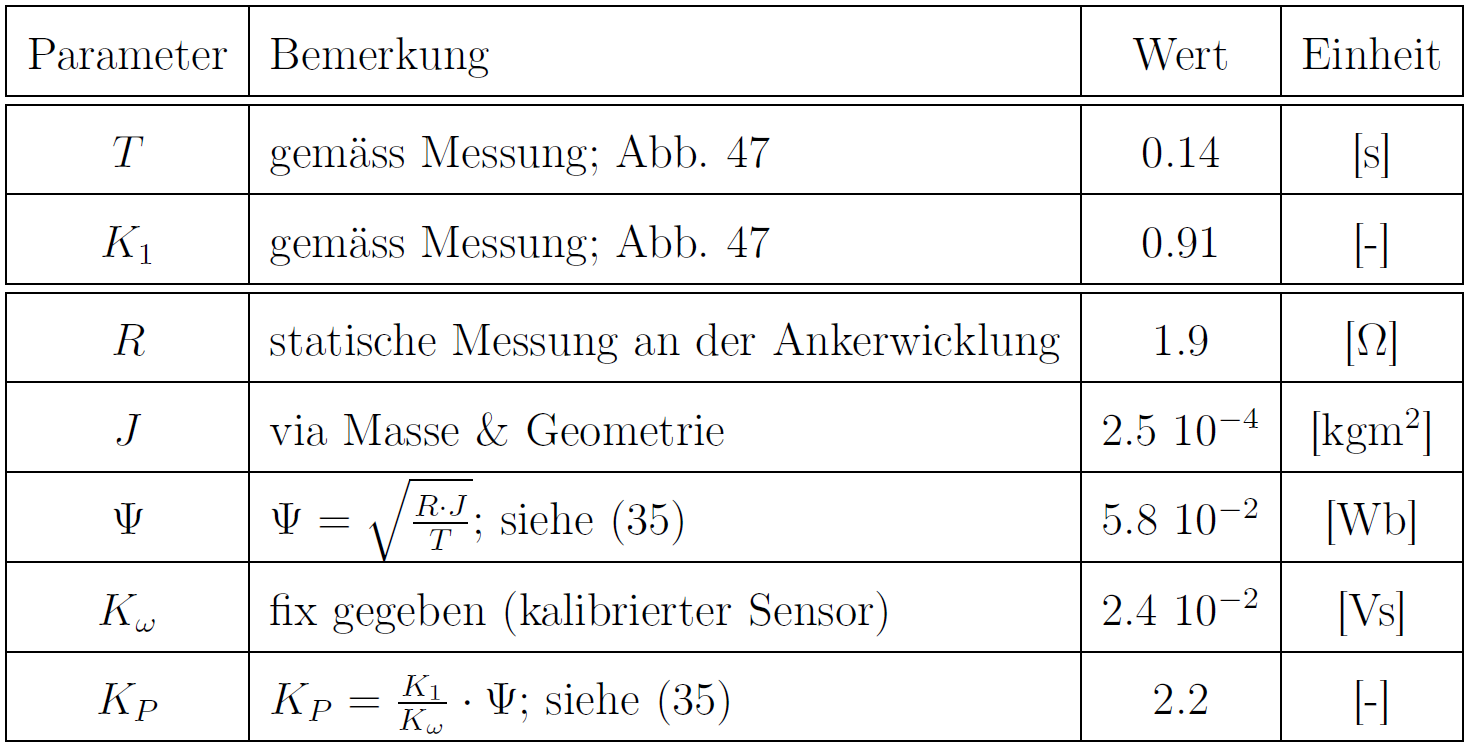
\includegraphics[width=\columnwidth]{images/gleichstrommodell_parameter.png}
    $M_{L1} = 4.8 \cdot 10^{-2} \, [\newton \meter]$
\end{minipage}


\subsection{Gleichstromantrieb mit Steuerung}{148-149}

Die Grösse $\omega$ soll im \textbf{steady-state} gesteuert werden \textrightarrow\ Ableitungen 0, keine Störungen \\
Zu steuern: $\omega = 25 \cdot 2 \pi$, $K_{\omega} \cdot \omega = y = 3.77 \, \volt$ \textrightarrow\ Finde Wert der Eingangsgrösse $u(t)$
$$ \boxed{ \text{Im steady-state: } \xcancel{ \underbrace{\frac{R \cdot J}{\Psi^2}}_{T} \dot{y}(t) } + y_{\rm stat}(t) = \underbrace{\frac{K_P \cdot K_{\omega}}{\Psi}}_{K_1} u(t)
    -  \xcancel{ \underbrace{\frac{R \cdot K_{\omega}}{\Psi^2}}_{K_2} M_L(t) } }$$

$$ y_{\rm stat} = \frac{K_P \cdot K_{\omega}}{\Psi} u_{\rm stat} \qquad  \underrightarrow{y_{\rm stat} = K_{\omega} \cdot \omega } \qquad 
    \omega_{\rm stat} = \frac{K_p}{\Psi} u_{\rm stat}  $$
$$ \text{\textrightarrow\ } u_{\rm stat} = \frac{\Psi}{K_P} \omega_{\rm stat}  = \frac{\Psi}{K_P} 25 \cdot 2 \pi = 4.14 \, \volt \quad  $$


\subsubsection{Probleme der Steuerung}

\begin{minipage}[c]{0.4\columnwidth}
    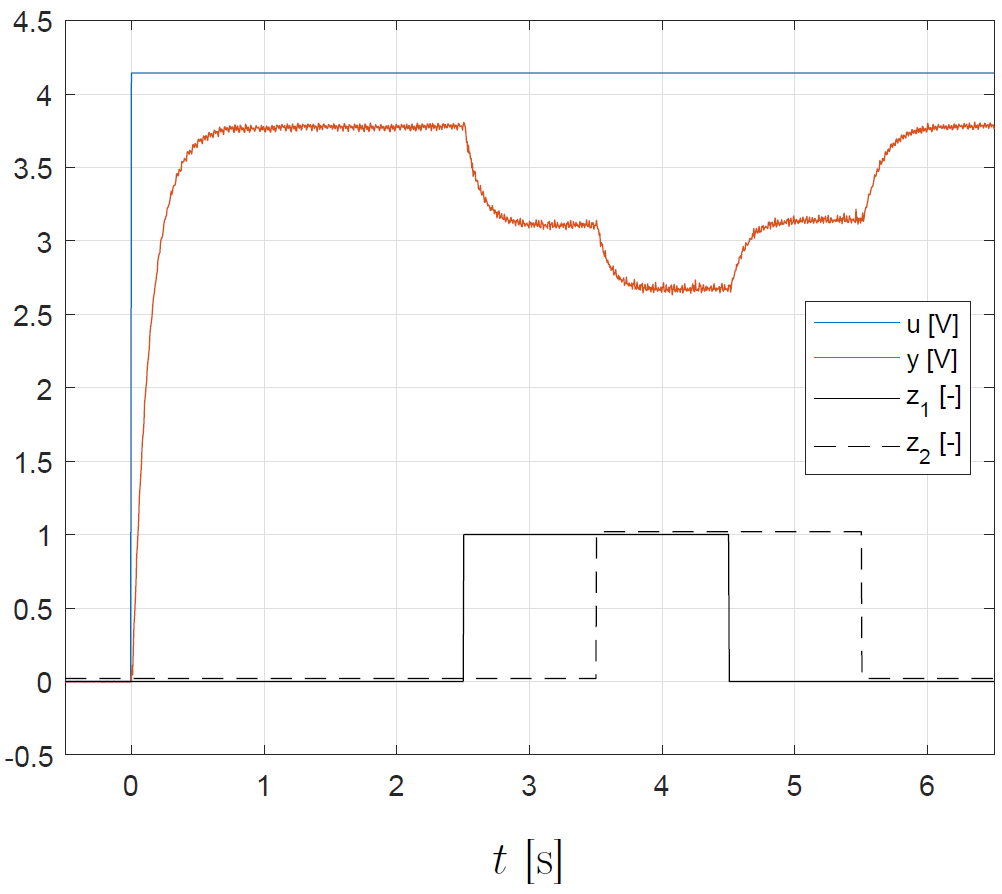
\includegraphics[width=\columnwidth]{images/gleichstromantrieb_steuerung_step-response.png}
\end{minipage}
\hfill
\begin{minipage}[c]{0.48\columnwidth}
    \begin{itemize}
        \item Endwert wird zwar erreicht, aber wenn $K_P$ oder $\Psi$ variieren wird dies nicht mehr der Fall sein
        \item Die Drehzahländerung ist 'langsam' (gemäss Zeitkonstante $T$). (Ein höheres $u$ zu Beginn könnte $T$ verkürzen)
        \item \textbf{Die Steuerung reagiert nicht auf die Störungen!}
    \end{itemize}
\end{minipage}


\subsection{Gleichstromantrieb mit P-Regler}{149-150}
\label{P-Regler}

\begin{minipage}[c]{0.4\columnwidth}
    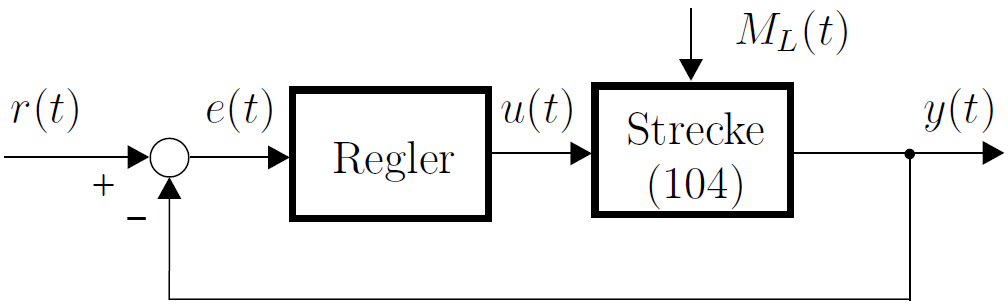
\includegraphics[width=\columnwidth]{images/gleichstromantrieb_p-regler.png}
\end{minipage}
\hfill
\begin{minipage}[c]{0.48\columnwidth}
    $$ u(t) = K_R \cdot e(t) = K_R \cdot ( r(t) - y(t) )$$
\end{minipage}

$$ \boxed{ \text{Geschlossener Regelkreis: } \underbrace{\frac{T}{1 + K_1 K_R}}_{T_f} \dot{y}(t) + y(t) = \underbrace{\frac{K_1 K_R}{1 + K_1 K_R}}_{K_f} r(t)
    - \underbrace{\frac{K_2}{1 + K_1 K_R}}_{K_z} M_L(t) } $$

Damit der Sollwert $r(t)$ erreicht wird (wenn keine Störung $M_L(t)$ vorhanden ist), muss $K_F = 1$ sein
\textrightarrow\ $K_R$ muss sehr gross sein


\subsubsection{Eigenschaften des P-Reglers}

\begin{minipage}[c]{0.4\columnwidth}
    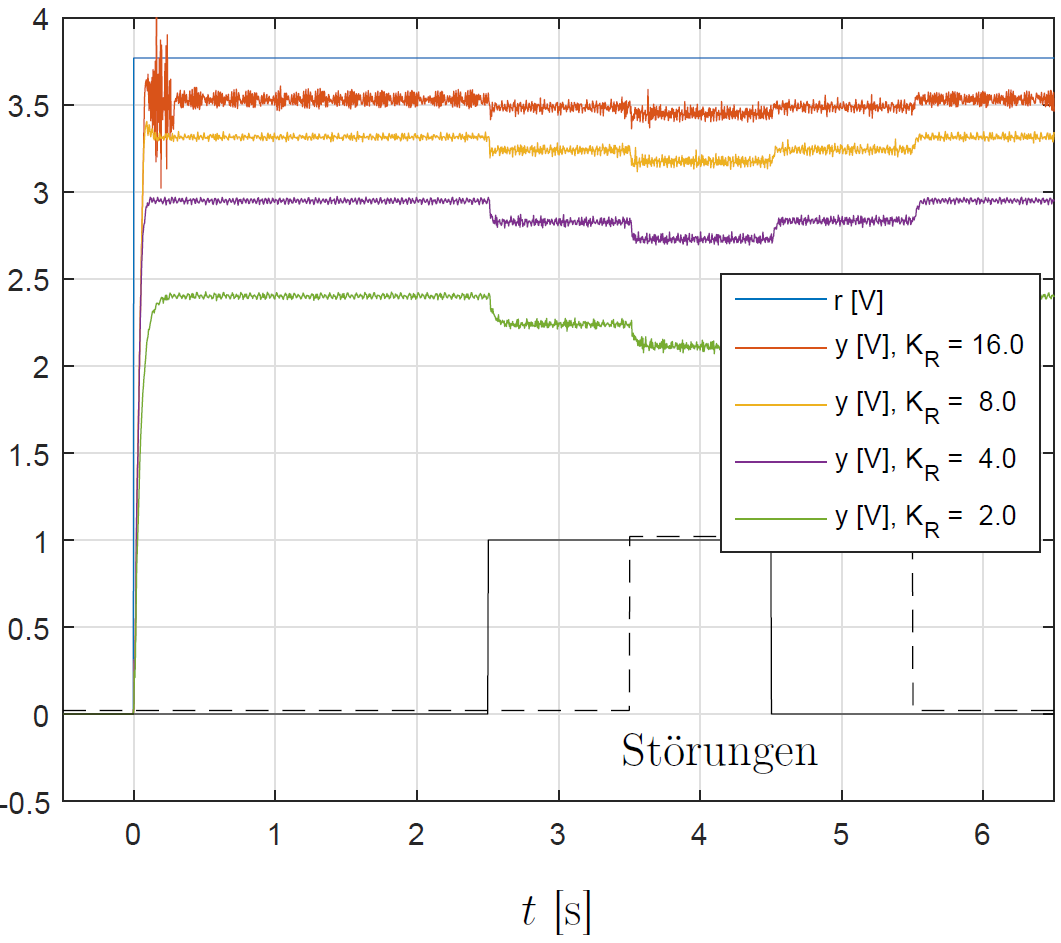
\includegraphics[width=\columnwidth]{images/gleichstromantrieb_p-regler_step-response.png}
\end{minipage}
\hfill
\begin{minipage}[c]{0.58\columnwidth}
    \begin{itemize}
        \item Für $K_R \to \infty$ werden die Zeitkonstante $T_f$ und der Einfluss der Störung $M_L(t)$ beliebig klein \\
            \textrightarrow\ DGL konvergiert zu $y(t) = r(t)$
        \item Für kleine $K_R$ wird Endwert nicht erreicht \\
            \textrightarrow\ statischer Fehler
        \item Stellgrösse $u(t)$ sättigt aufgrund von physikalischen Gegebenheiten \textrightarrow\ Prozess wird \textbf{nichtlinear}
            \textrightarrow\ Überschwinger
        \item Messrauschen wird ebenfalls verstärkt (P-Regler verstärt \textbf{alle} Frequenzen) 
    \end{itemize}
\end{minipage}

\textrightarrow\ \textbf{Es bleibt ein stationärer Fehler!} Dafür reagiert der P-Regler schnell.


\subsection{Gleichstromantrieb mit I-Regler}{151-152}

\begin{minipage}[t]{0.48\columnwidth}
    \begin{center}
        \myul{I-Regler ($K_R$ einstellbar)}
    \end{center}
    $$ u(t) = K_R \int\limits_0^t \underbrace{ r(\tau) - y(\tau)}_{e(\tau)} \, \diff \tau $$
\end{minipage}
\hfill
\begin{minipage}[t]{0.48\columnwidth}
    \begin{center}
        \myul{E-Motor (Strecke, $\text{PT}_1$-System)}
    \end{center}
    $$ T \cdot \dot{y}(t) + y(t) = K_1 \cdot u(t) - K_2 \cdot M_L(t) $$
\end{minipage}

\textrightarrow\ $u(t)$ von I-Regler in Gleichung der Strecke einsetzen, ableiten, umsortieren

$$ \boxed{ \text{PT}_2 \text{-System:} \quad \underbrace{ \frac{T}{K_1 \cdot K_R} }_{T_f^2} \ddot{y}(t) + \underbrace{ \frac{1}{K_1 \cdot K_R} }_{2 \zeta_f T_f} \dot{y}(t) + y(t) 
    = \underbrace{1}_{K_f} r(t) - \frac{K_2}{K_1 \cdot K_R} \dot{M}_L(t) } $$


\subsubsection{Eigenschaften des I-Reglers}

\begin{minipage}[c]{0.48\columnwidth}
    \begin{itemize}
        \item $T_f = \sqrt{ \frac{T}{K_1 \cdot K_R} }$, $\zeta_f = \frac{1}{2 \sqrt{T K_1 K_R}}$
        \item \textbf{Der Integrator sorgt dafür, dass im steady-state kein stationärer Fehler auftritt} ($e(t) = 0$)
        \item Für grosse $K_R$ wird $T_f$ klein, die Sprungantwort schneller (erwünscht)
        \item Für grosse $K_R$ wird $\zeta_f$ klein, die Überhöhung grösser (unerwünscht)
        \item \textrightarrow\ Kompromiss finden
    \end{itemize}
\end{minipage}
\hfill
\begin{minipage}[c]{0.48\columnwidth}
    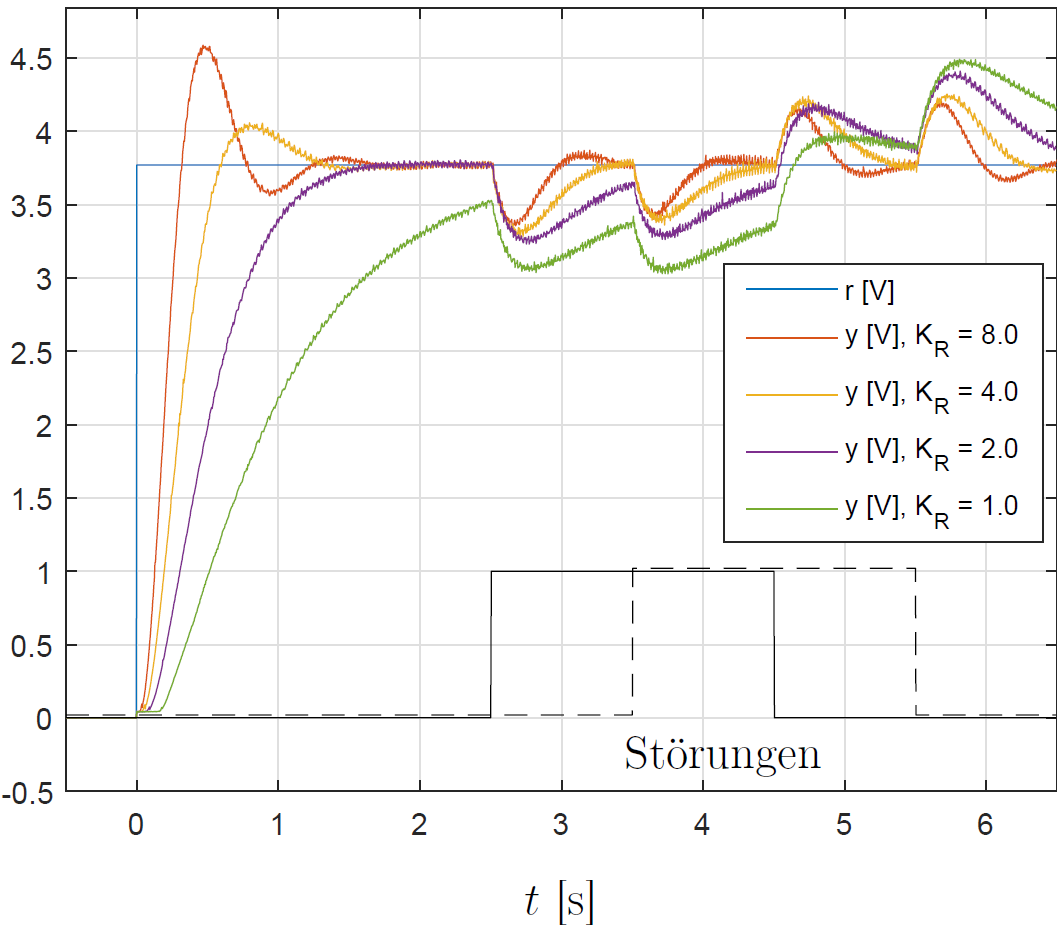
\includegraphics[width=\columnwidth]{images/gleichstromantrieb_i-regler_step_response.png}
\end{minipage}


\subsection{Gleichstromantrieb mit PI-Regler}{152-154}

Vorteile von P-Regler und I-Regler sollen kombiniert werden:
\begin{itemize}
    \item P-Regler für schnelle Reaktion
    \item I-Regler für statische Fehlerunterdrückung
        \textrightarrow\ Parameter $K_R$ und $T_N$ einstellbar
\end{itemize}

\vspace{-0.4cm}
$$ \text{PI-Regler:} \quad u(t) = \frac{1}{T_N} \left\lgroup \int\limits_0^t e(\tau) \, \diff \tau + e(t) \right\rgroup K_R
    \; \laplace \; U(s) = \frac{1}{T_N} \left\lgroup \frac{1}{s} E(s) + E(s) \right\rgroup K_R $$
$$ \text{E-Motor:} \quad T \dot{y}(t) + y(t) = K_1 u(t) - K_2 M_L(t) 
    \; \laplace \; T s Y(s) + Y(s) = K_1 U(s) - \cancel{ K_2 M_L(s)} $$

\vspace{-0.3cm}
\begin{minipage}[t]{0.53\columnwidth}
    $$ \text{UTF Regler: } G_R(s) = \frac{U(s)}{E(s)} = K_R \left\lgroup \frac{1}{T_N} \frac{1}{s} + 1 \right\rgroup $$
\end{minipage}
\hfill
\begin{minipage}[t]{0.46\columnwidth}
    $$ \text{UTF Strecke: } G_S(s) = \frac{Y(s)}{U(s)} = \frac{K_1}{T s + 1} $$
\end{minipage}

Der  Parameter $T_N$ des PI-Reglers wird so gewählt, dass der \textbf{offene Regelkreis} $G_0(s)$ einem \textbf{Integrator} entspricht!
\textrightarrow\ \textbf{Pol-Nullstellenkürzung!}

$$ G_0(s) = G_R(s) \cdot G_S(s) = K_R \frac{1 + T_N s}{T_N s} \cdot \frac{K_1}{T s + 1} \overset{T_N = T}{=} K_R \frac{K_1}{T_N s} $$

Für den \textbf{geschlossenen Regelkreis} ergibt sich somit ein $\text{PT}_1$-System mit Verstärkung $1$\\
(\textrightarrow\ kein statischer Fehler im steady-state). Die Zeitkonstante $T_{\rm geschl}$ wird mit $K_R$ des Reglers eingestellt.

$$ G_f(s) = \frac{G_0(s)}{1 + G_0(s)} =  \frac{\frac{K_R  K_1}{T_N s} }{1 \frac{K_R  K_1}{T_N s}} = \frac{K_R K_1}{T_N s + K_1 K_R} = \frac{1}{\frac{T_N}{K_R  K_1}s + 1} $$


\subsubsection{Pol-Nullstellenkürzung}

Wird durchgeführt, um den \textbf{offenen Regelkreis} zu vereinfachen. Pole und Nullstellen der Strecke werden mit einer geeigneten
Wahl der Parameter des Reglers kompensiert. \\
\textrightarrow\ \textbf{Idealfall: offener Regelkreis verhält sich wie ein Integrator.}

\begin{itemize}
    \item Betrachtung UTF des offenen Regelkreises
    \item Parameter des Reglers so wählen, dass man Polstelle mit einer Nullstelle kürzen kann \\
        \textrightarrow\ Diejenige Polstelle, welche am frühesten 'zündet', ist bevorzugt zu kürzen!
\end{itemize}


\subsubsection{Eigenschaften des PI-Reglers}

\begin{minipage}[c]{0.48\columnwidth}
    \begin{itemize}
        \item Zeitkonstante und Verstärkung unabhängig voneinander einstellbar
        \item Kein Überschwingen
        \item \textbf{Konstante Störungen werde unterdrückt (kein steady-state Fehler)}
        \item Grosse Verstärkung führt noch immer zu Sättigung
        \item Effekt des Rauschens eher harmlos, weil kleine Verstärkungen gewählt werden können
        \item $\Phi_{\rm RES} = 90 \degree$ und $K_{\rm RES} = \infty$
    \end{itemize}
\end{minipage}
\hfill
\begin{minipage}[c]{0.45\columnwidth}
    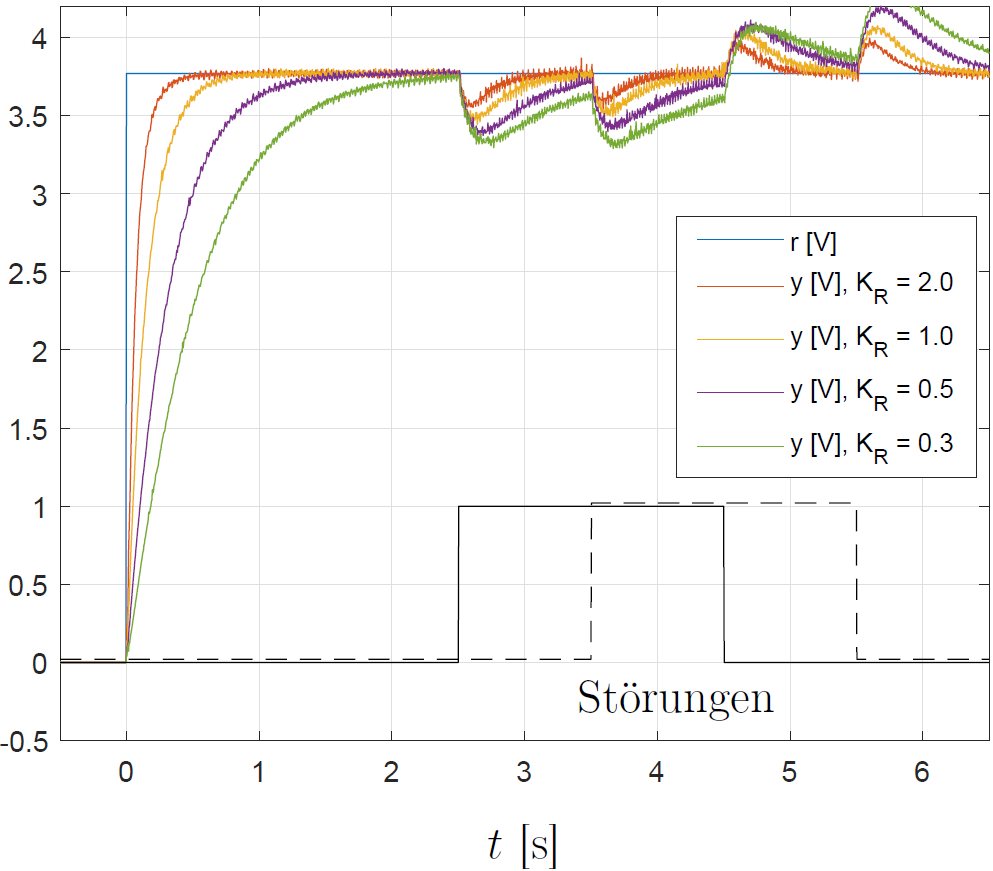
\includegraphics[width=\columnwidth]{images/gleichstromantrieb_pi-regler_step_response.png}
\end{minipage}


\subsection{Gleichstromantrieb mit PID / PD-Regler}{155}

\textbf{Der Regelkreis kann nicht weiter optimiert werden!} Der offenere Regelkreis entspricht bereits einem \textbf{Integrator},
was der \textbf{Idealfall} ist. 

Ein D-Anteil $\text{DT}_1$ wäre ungünstig, weil

\begin{itemize}
    \item Verstärkung von hohen Frequenzen \textrightarrow\ Erhöhung des Rauschens
    \item Verbesserung der Phasenreserve \textrightarrow\ unnötig bei $\Phi_{\rm RES} = 90 \degree$
\end{itemize}

Allenfalls sinnvoll wäre ein Tiefpassfilter für den P-Anteil ($\text{PT}_1$ statt P), um das Rauschen der Stellgrösse zu 
verkleinern \textrightarrow\ Reduktion der Phasenreserve!


\subsection{Gleichstromantrieb mit Totzeit mit PI-Regler}{157-159}

Das bisherige Modell der Strecke soll um eine Totzeit $T_t$ erweitert werden. Als Regler wird weiterhin ein PI-Regler eingesetzt.
Die Ergebnisse werden dadurch massiv schlechter!

$$ \text{UTF Stecke mit Totzeit} \quad G_S(s) = \frac{K_1}{s + 1} e^{-s T_t} $$
$$ \text{UTF Regelkreis} \quad G_0(s) = G_S(s) \cdot G_R(s) = \frac{K_1}{s + 1} e^{-s T_t} \cdot K_R \frac{1 + T_N s}{T_N s}
    \overset{T_N = T}{=} \frac{K_1 K_R}{s T} e^{-s T_t} $$

Die UTF des offenen Regelkreises $G_0(s)$ entspricht keinem Integrator mehr. Somit wird die UTF des geschossenen Regelkreises 
$G_f(s)$ keinem $\text{PT}_1$-System mehr entsprechen. 


\subsubsection{Effekte im Bode- und Nyquistdiagramm / Sprungantwort}

\begin{itemize}
    \item Amplitudengang unverändert, gleiche Durchtrittsfrequenz
    \item Phasengang wird schlechter (zusätzliche Phasenverzögerung), die $-180 \degree$ Phase wird bei tieferer
        Frequenz erreicht - die Verstärkungsreserve sinkt dadurch
    \item Die Phase bei der Durchtrittsfrequenz ist negativer, die Phasenreserve sinkt
\end{itemize}

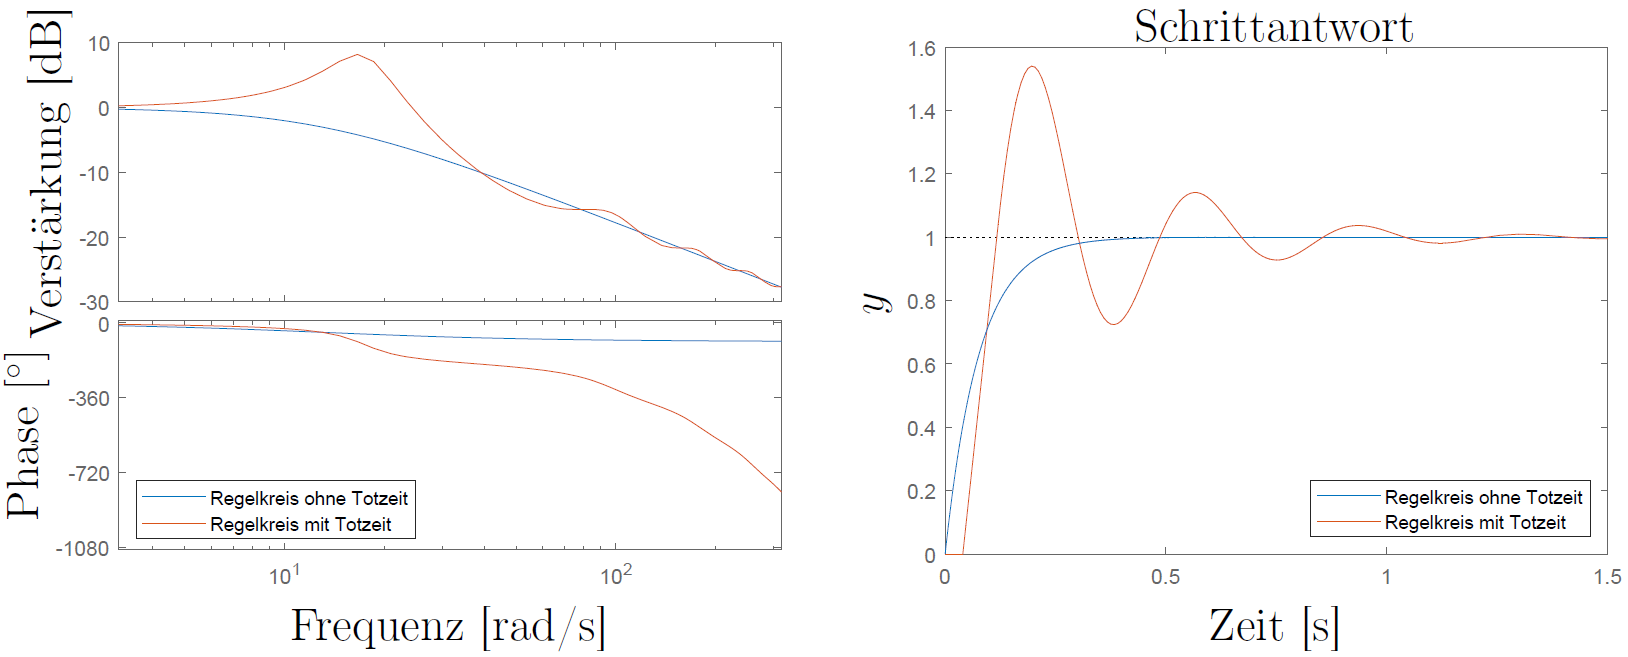
\includegraphics[width=\columnwidth]{images/gleichstromantrieb_pi-regler_totzeit_step_response.png}


\subsection{Gleichstromantrieb mit Totzeit mit PID-Regler}{160-162}

Um der Totzeit $T_t$ entgegenzuwirken, wird dem PI-Regler ein Lead-Glied (entspricht einem PD-Regler) in serie geschaltet 
\textrightarrow\ PID-Regler in multiplikativer Form (Abschnitt~\ref{PID-Regler multiplikative Form})

\medskip
Dies hat folgende Effekte:
\begin{outline}
    \1 Nyquistkurve wird bei der Durchtrittsfrequenz aktiv durch den Regler 'zurückgedreht' 
        \2 Effekt der Totzeit nicht für alle Frequenzen kompensieren, sondern in einem bestimmten Frequenzbereich
        \2 Im Bodediagramm: Phase bei $0 \, \deci \bel$ 
    \1 Serieschaltung eines Lead-Glieds (PD-Regler) zum PI-Regler \textrightarrow\ PID-Regler \\
        \textrightarrow\ Lead-Glied siehe Abschnitt ~\ref{Lead-Lag-Glied}
\end{outline}


\subsubsection{Auswirkungen des Lead-Glieds / PD-Reglers}

\begin{itemize}
    \item Phase und Verstärkung werden angehoben
    \item Zeitkonstante wird kleiner (Regler wird schneller)
\end{itemize}

\begin{minipage}[c]{0.4\columnwidth}
    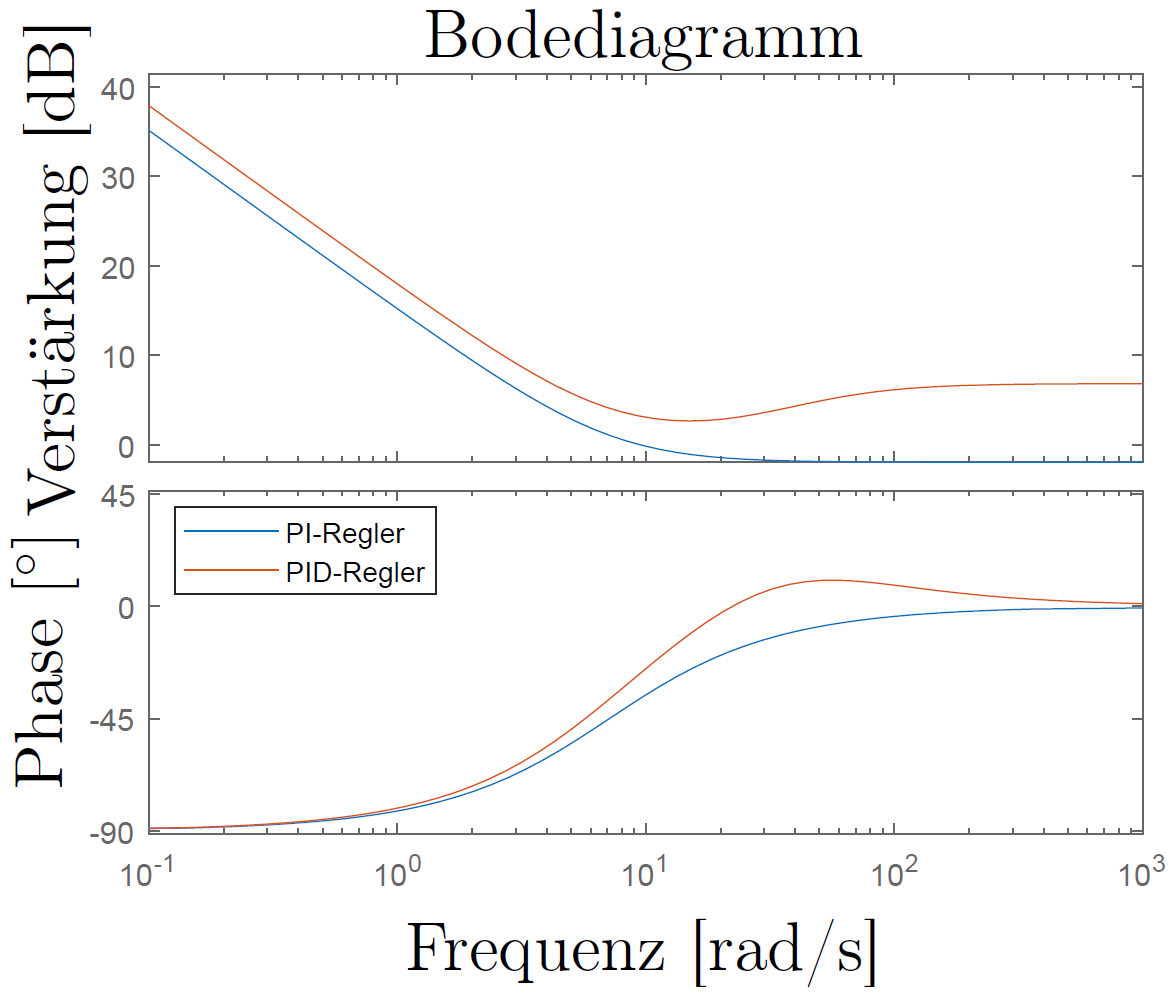
\includegraphics[width=\columnwidth]{images/gleichstromantrieb_pid-regler_bodediagramm.png}
\end{minipage}
\hfill
\begin{minipage}[c]{0.4\columnwidth}
    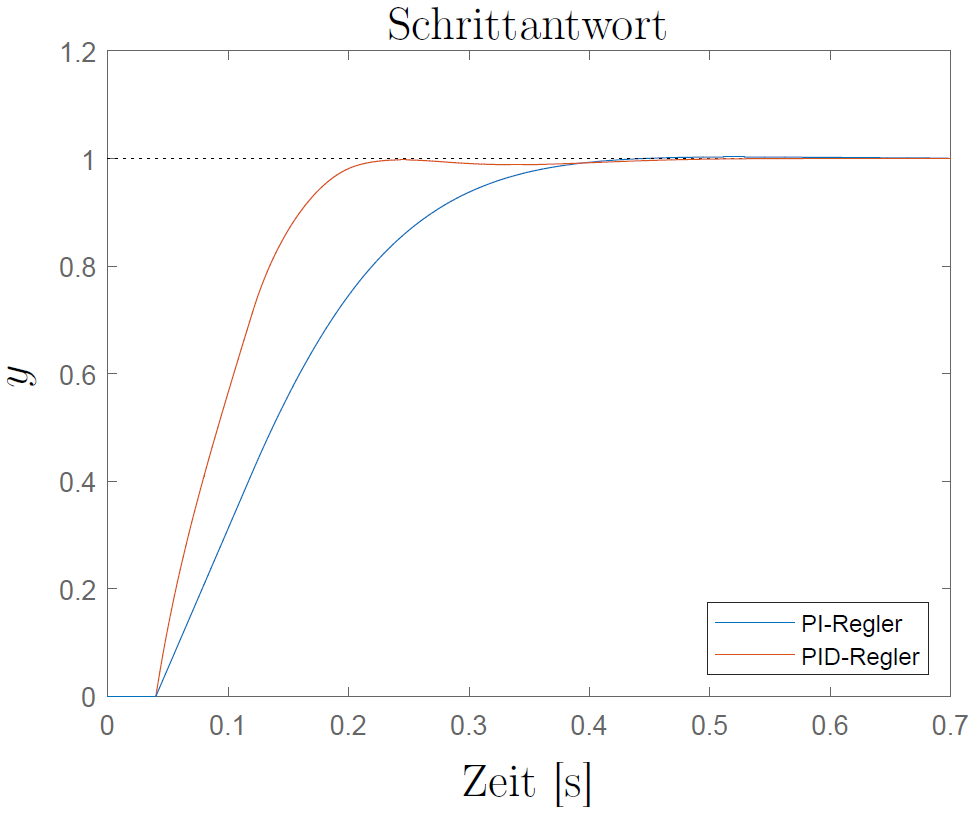
\includegraphics[width=\columnwidth]{images/gleichstromantrieb_pid-regler_step_response.png}
\end{minipage}


        % \section{Implementierung analoger Regler}

\textbf{Voraussetung:} Regler ist ausgelegt (Parameter und Struktur des Reglers bekannt)


\subsection{Struktur allgemeiner Frequenzgang eines Reglers}

Der Frequenzgang des Reglers $G_R(\jimg \omega)$ mit ($m \leq n$) ist beschrieben durch
$$ G_R(\jimg \omega) = \frac{U(\jimg \omega)}{E(\jimg \omega)} 
    = \frac{b_n (\jimg \omega)^n + b_{n-1}(\jimg \omega)^{n-1} + \ldots + b_0}{(\jimg \omega)^n + a_{n-1}(\jimg \omega)^{n-1} + \ldots + a_0} 
    = \frac{b_n + b_{n-1} \frac{1}{\jimg \omega} + \ldots + b_0 \frac{1}{(\jimg \omega)^n}}{1 + a_{n-1} \frac{1}{\jimg \omega} + \ldots + a_0 \frac{1}{(\jimg \omega)^n}} $$

\begin{minipage}[c]{0.55\columnwidth}
    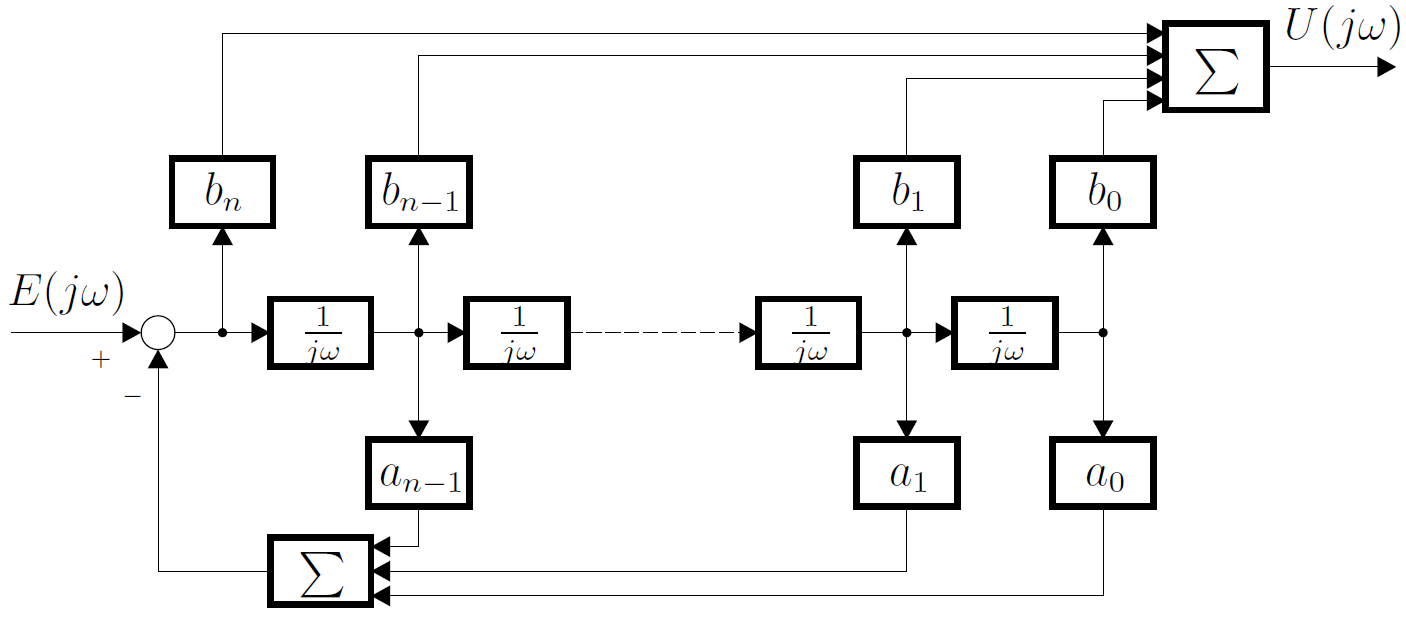
\includegraphics[width=\columnwidth]{images/struktur_allgemeiner_frequenzgang.png}
\end{minipage}
\hfill
\begin{minipage}[c]{0.43\columnwidth}
    Ein jeder solcher Frequenzgang besteht nur aus \textbf{Integratoren, Summatoren und Verstärkungen}. 
    Diese Grundglieder können mit OpAmp-Schaltungen realisiert werden.
\end{minipage}


\subsection{Grundschaltungen mit OpAmps}

\textbf{Hinweis:} Die folgenden Betrachtungen gelten für \textbf{ideale OpAmps}!


\subsubsection{Summator}

\begin{minipage}[c]{0.35\columnwidth}
    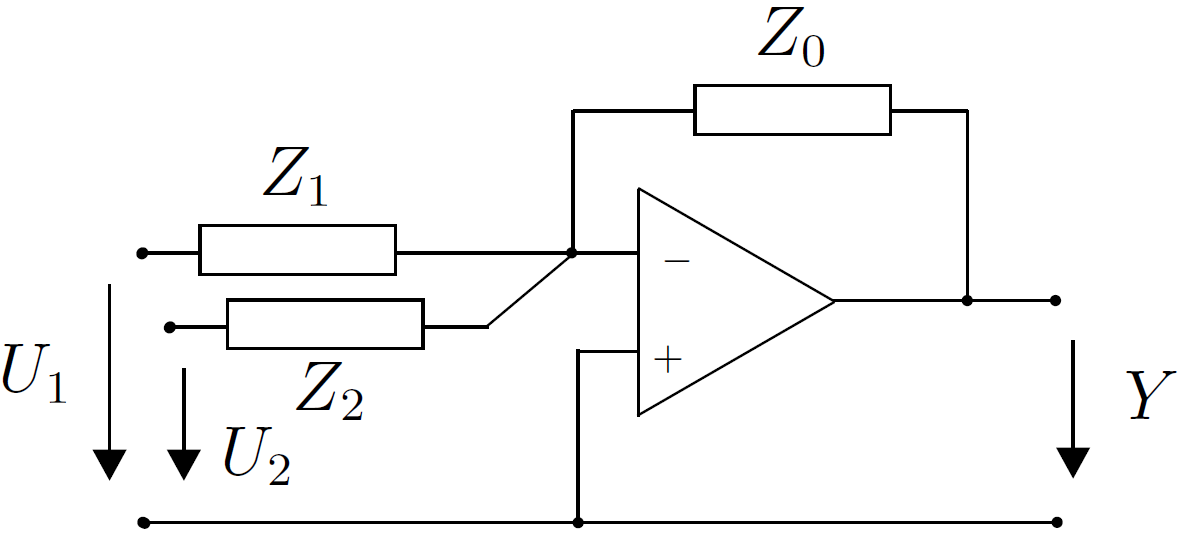
\includegraphics[width=\columnwidth]{images/opamp_grundschaltung_2_eingaenge.png}
\end{minipage}
\hfill
\begin{minipage}[c]{0.62\columnwidth}
    % \raggedright
    $$ Y = - \frac{Z_0}{Z_1} \cdot U_1 - \frac{Z_0}{Z_2} \cdot U_2 $$
    \textrightarrow Auf beliebig viele Eingaänge erweiterbar
\end{minipage}


\subsubsection{Integrierer}

\begin{minipage}[c]{0.35\columnwidth}
    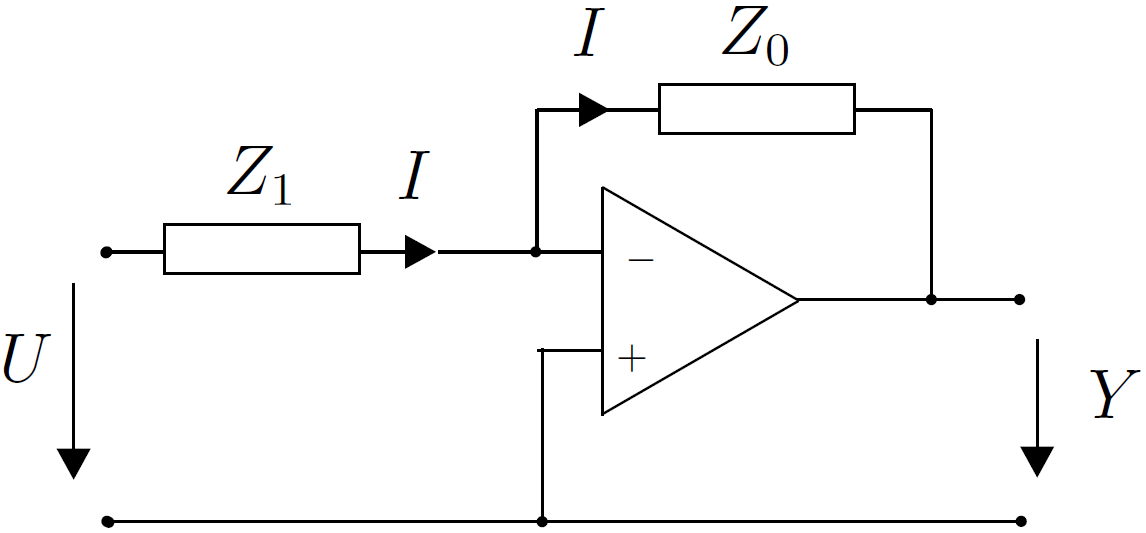
\includegraphics[width=\columnwidth]{images/opamp_grundschaltung_1_eingang.png}
\end{minipage}
\hfill
\begin{minipage}[c]{0.62\columnwidth}
    $$ Z_0 = \frac{1}{\jimg \omega C} \text{ (Kondensator) } \qquad  Z_1 = R $$
    $$ Y = - \frac{1}{\jimg \omega R C} \cdot U \quad \Rightarrow Y =  - \frac{1}{\jimg \omega R_1 C} \cdot U_1 - \frac{1}{\jimg \omega R_2 C} \cdot U_2 $$
\end{minipage}          

\vspace{0.2cm}
\begin{itemize}
        \item Für einen oder mehrere Eingänge geeignet
        \item Braucht 'Reset'-Schaltung, um Kondensator zu entladen
        \item \textbf{Anti-Wind-Up} durch Sättigung der Speisespannung \textbf{gegeben}
\end{itemize}


\subsubsection{P-Glied (passiv)}

\begin{minipage}[c]{0.28\columnwidth}
    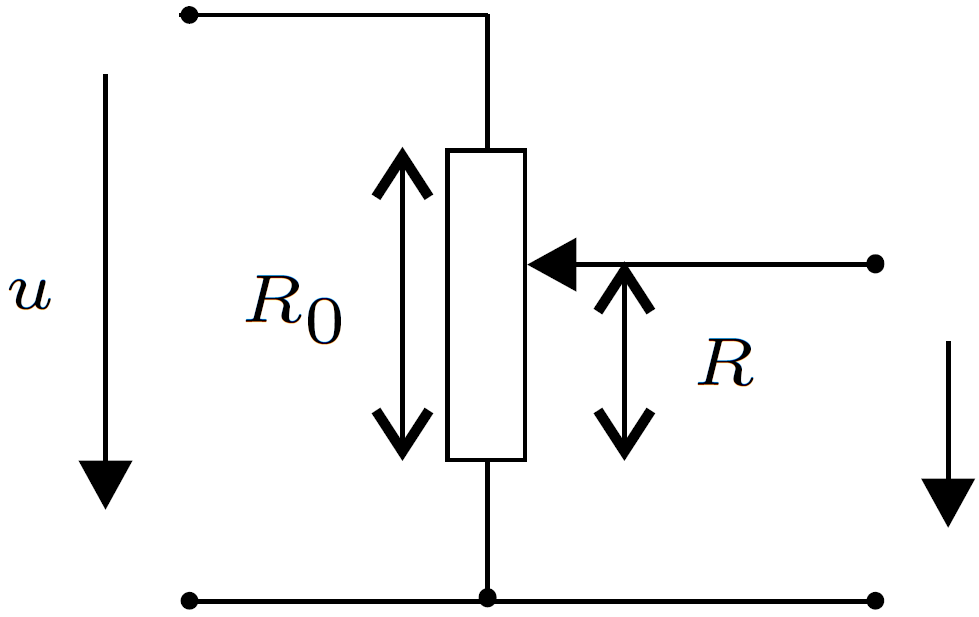
\includegraphics[width=\columnwidth]{images/spannungsteiler.png}
\end{minipage}
\hfill
\begin{minipage}[c]{0.7\columnwidth}
    % $$ y = u \cdot \frac{R}{R_0} $$

    \begin{tabular}{ll}
        Verstärkung $< 1$  & \textrightarrow\ passiver Spannungsteiler \\
        Verstärkung $> 1$  & \textrightarrow\ OpAmp-Schaltung \\
    \end{tabular}

    \vspace{0.2cm}

    \begin{itemize}
        \item OpAmps sollten als Summierer oder Integratoren mit definierter Verstärkung aufgebaut werden
        \item Vor Eingänge des OpAmps passive Spannungsteiler setzen
    \end{itemize}
\end{minipage}


\subsection{Varianten analoger PID-Schaltungen}

\subsubsection{Variante 1 (gemischt)}

\begin{minipage}[c]{0.48\columnwidth}
    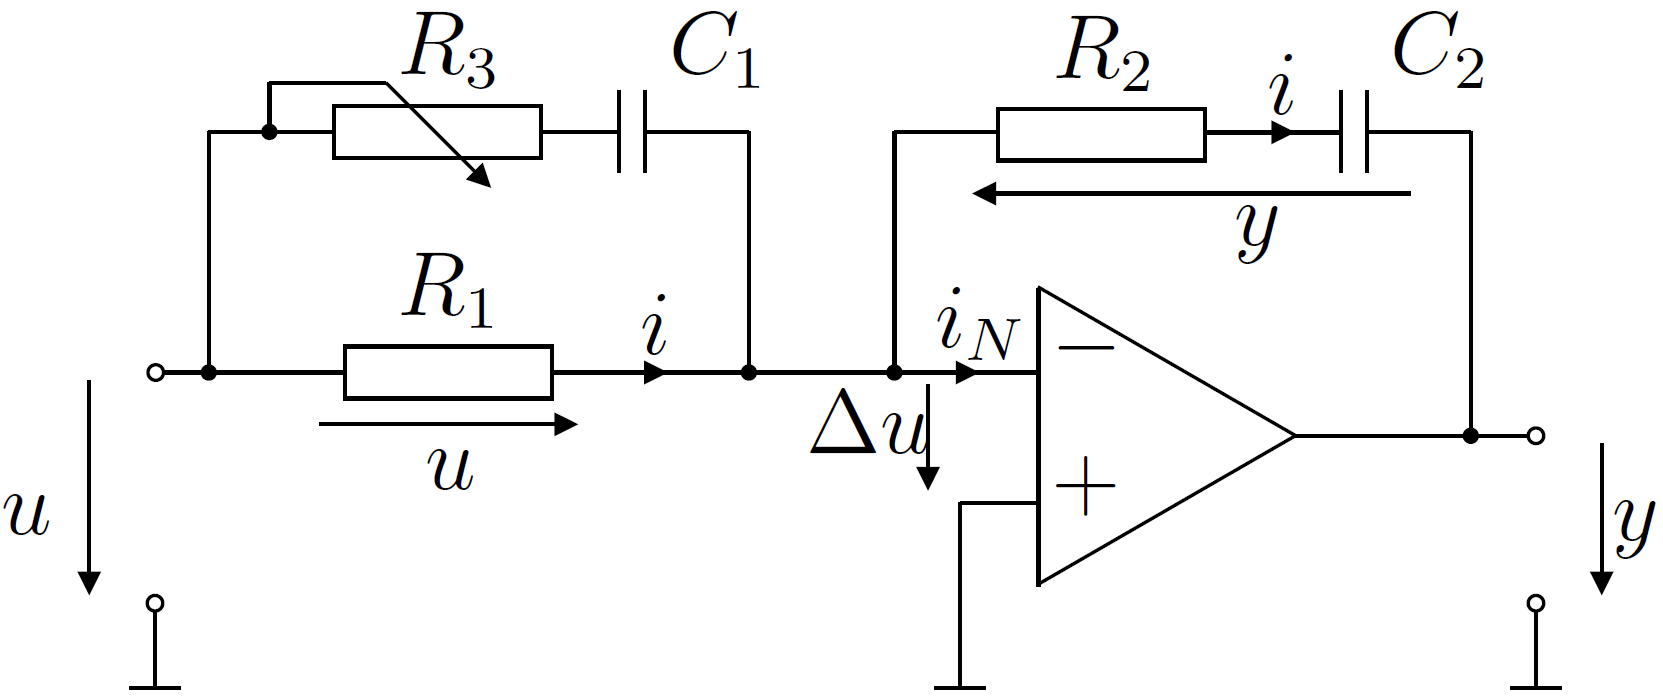
\includegraphics[width=\columnwidth]{images/realisierung_pid-regler_variante_1.png}
\end{minipage}
\hfill
\begin{minipage}[c]{0.48\columnwidth}
    \begin{tabular}{ll}
        $R_1$   & Proportional (P-Anteil) \\
        $C_1$   & Ableitung (D-Anteil) \\
        $R_3$   & Filterkonstante der Ableitung \\
                & \textrightarrow $R_1$ und $C_1$ bilden $\text{DT}_1$-Anteil \\
        $C_2$   & Integral (I-Anteil) \\
    \end{tabular}
    \vspace{0.2cm}

    \textrightarrow Betrachtung als Summator mit $Z_0$ und $Z_1$ möglich
\end{minipage}


\subsubsection{Variante 2 (Parallelform)}

\begin{minipage}[c]{0.45\columnwidth}
    \includegraphics[width=\columnwidth]{images/realisierung_pid-regler_variante_2.png}
\end{minipage}
\hfill
\begin{minipage}[c]{0.52\columnwidth}
    Der Frequenzgang $G(\jimg \omega)$ des Reglers lautet
    $$ \frac{U_{\rm PID}}{U_E} = \underbrace{ \frac{R_2}{R_1} }_{K_R} \cdot \Bigl( 1 + \frac{1}{\jimg \omega \underbrace{C_I R_I}_{T_N}} 
        + \jimg \omega \underbrace{ C_D R_D }_{T_V} \Bigr) $$
    Durch Einbau eines Widerstands an der Stelle \textbf{A} wird der der PID-Regler zu einem $\text{PIDT}_1$-Regler.
\end{minipage}


        \section{Implementierung digitaler Regler}

Heutzutags werden fast nur noch digitale Regler implementiert. Gründe hierfür sind:

\begin{itemize}
    \item Verarbeitung digitaler Signale ist flexibel
    \item Speichung und Übertragung digitaler Signale ist einfach
    \item Komponenten (Rechner, Wandler) für ditigale Umsetzung werden immer günstiger
\end{itemize}


\subsection{Aufbau digitaler Regelkreis}{183}

\begin{minipage}[c]{0.63\columnwidth}
    \includegraphics[width=\columnwidth]{images/regelkreis_mit_digitalregler.png}
\end{minipage}
\hfill
\begin{minipage}[c]{0.35\columnwidth}
    \begin{itemize}
        \item Strecke ändert nicht
        \item Regler arbeitet \textbf{zeitdiskret}
    \end{itemize}
\end{minipage}


\subsubsection{Signale im digitalen Regelkreis}{184}

\begin{center}
    \includegraphics[width=0.75\columnwidth]{images/digitaler_regelkreis_signaltypen.png}
\end{center}

\begin{outline}
    \1 Sensorseitig wird periodisch die Regelgrösse abgetastet (zuvor TP-filtern)
        \2 \textbf{TP:} Analoges Tiefpassfilter \textrightarrow\ Anti-Aliasing
    \1 Aktorseitig wird mit \textbf{ZOH}-Halteglied (Zero-Order-Hold) aus dem diskreten Signal $u(k)$ eine kontinuierliche Funktion $u(t)$ erzeugt 
\end{outline}


\subsubsection{Quantisierung}{185}

Das Signal eines ditialen Reglers ist sowohl \textbf{zeitdiskret} als auch \textbf{wertdiskret}.

\medskip
\begin{minipage}[c]{0.49\columnwidth}
    \includegraphics[width=\columnwidth]{images/abtastung.png}
\end{minipage}
\hfill
\begin{minipage}[c]{0.5\columnwidth}
    \raggedright%
    \textbf{\myul{Abtastzeit $T$}}

    \begin{outline}
        \1 $T$ zu gross gewählt
            \2 Schlechtes Führungsverhalten (Überschwingen)
        \1 $T$ zu klein gewählt
            \2 Möglicherweise numerische Probleme
            \2 Höhere Anforderungen an Sensor, Aktor, Wandler und Digitalrechner
    \end{outline}


    \textbf{\myul{Sättigung und Quantisierung}}

    \begin{outline}
        \1 Grobe Quantisierung
            \2 Nichtlineare Reglerung
        \1 Feine Quantisierung
            \2 Keinen (negativen) Einfluss auf Regler 
    \end{outline}
\end{minipage}


\subsection{Entwurfsverfahren}{186}

\begin{minipage}[c]{0.45\columnwidth}
    \includegraphics[width=\columnwidth]{images/direkter_indirekter_reglerentwurf_digital.png}  
\end{minipage}
\hfill
\begin{minipage}[c]{0.53\columnwidth}
    \begin{outline}
        \1  \textbf{Indirekter digitaler Reglerentwurf}
            \2 $G_S(\jimg \omega)$ \textrightarrow\ 'links herum' \textrightarrow\ $G_{R,I}(z)$
        \1 Direkter digitaler Reglerentwurf
            \2 $G_S(\jimg \omega)$ \textrightarrow\ 'rechts herum' \textrightarrow\ $G_{R,D}(z)$
            \2 'Digitale Natur' des Reglers von Anfang an berücksichtigt
    \end{outline}
\end{minipage}

\textbf{Hinweis:} Normalerweise sind die resultierenden Regler nicht identisch: $G_{R,I}(z) \neq G_{R,D}(z)$


\subsection{Diskretisierung eines Reglers}{188}

Ein kontinuierlicher Regler (hier I-Regler) weist folgendes Verhalten auf:
$$ u(t) = K_R \cdot \int\limits_0^t e(\tau) \, \diff \tau $$

Der entsprechende zeitdiskrete Regler kann \textbf{nicht exakt} gebildet werden, da $e(t)$ nur zu diskreten Zeitpunkten $e(kT)$ bekannt ist.
Geht man davon aus, dass $e(t)$ \textbf{nicht stakt ändert} (\textrightarrow\ geeignete Wahl der Abtastzeit $T$), dann kann $u(k)$
folgendermassen approximiert werden:

$$ u(k) = K_R \cdot \int\limits_0^{kT} e(\tau) \, \diff \tau
    = \underbrace{K_R \cdot \int\limits_0^{kT- T} e(\tau) \, \diff \tau}_{u(k-1)} 
    + \underbrace{K_R \cdot \int\limits_{kT-T}^{kT} e(\tau) \, \diff \tau}_{\approx A} $$


\subsubsection{Approximationen der Fläche $A$}

Die Fläche $A$ kann auf mehrere Arten approximiert werden:


\begin{minipage}[c]{0.3\columnwidth}
    \includegraphics[width=\columnwidth]{images/approximation_integration.png}
\end{minipage}
\hfill
\begin{minipage}[c]{0.68\columnwidth}
    \begin{tabular}{ll}
        Rechteckregel vorwärts (Euler)      & $ A = T \cdot e(k-1) $    \\
        Rechteckregel rüclwärts             & $ A = T \cdot e(k)$       \\
        \textbf{Trapezregel (Tustin)}       & $ A = T \cdot \frac{e(k-1) + e(k)}{1} $ 
    \end{tabular}
\end{minipage}

\vspace{0.2cm}
\textbf{Hinweis:} Für die Diskretisierung von Reglern wird die \textbf{Trapez-Approximation} verwendet, da diese am genausten ist.


\subsection{Vorgehen: Diskretisierung eines Reglers}

\begin{enumerate}
    \item Übertragungsfunktion des Reglers in $\jimg \omega$ aufstellen: $G_R(\jimg \omega) = ...$
    \item Wahl der Abtastzeit $T_S$ und einer Diskretisierungsmethode \\
        -- (typischerweise Tustin, weil am genausten)
    \item Substitution aller $\jimg \omega$ in der UTF durch Approximation in $z^{-1}$ \textrightarrow\ $G_{R, \, \rm diskret}(z) = ...$ \\
        -- Tustin: $\jimg \omega = \frac{2}{T} \frac{1 - z^{-1}}{1 + z^{-1}}$
    \item Umformen, damit Doppelbrüche verschwinden
    \item Ansatz: $G_{R, \, \rm diskret}(z) = \frac{U(z)}{E(z)}$ sortieren nach $U(z)$ und $E(z)$
    \item Differenzengleichung durch inverse Z-Transformation bestimmen
\end{enumerate}


\example{PI-Regler diskretisieren}

Gegeben sei die Übertragungsfunktion $G_R(\jimg \omega)$ eines \textbf{kontinuierlichen} Reglers.
Daraus soll die zu implementierende \textbf{Differenzengleichung} ermittelt werden.

$$ 1. \quad G_R(\jimg \omega) = K_R \cdot \frac{1 + T_N \jimg \omega}{T_N \jimg \omega} \quad {\textrightarrow\ }2. $$
$$ G_{R, \, \rm diskret}(z) \overset{3.}{=} K_R \cdot \frac{1 + T_N \frac{2}{T} \frac{1- z^{-1}}{1 + z^{-1}}}{T_N \frac{2}{T} \frac{1- z^{-1}}{1 + z^{-1}}} 
\overset{4.}{=} K_R \cdot \frac{T (1 + z^{-1}) + 2 T_N (1 - z^{-1})}{2 T_N (1- z^{-1})} = \frac{U(z)}{E(z)} $$
$$  5. \quad U(z) (1 - z^{-1}) = \frac{K_R}{2 T_N} \cdot E(z) \Big( T (1 + z^{-1}) + 2 T_N (1 - z^{-1}) \Big) $$
$$  6. \quad u(k) - u(k-1) = \frac{K_R}{2 T_N} \Big[ T \cdot e(k) + T \cdot e(k-1) + 2 T_N \cdot e(k) - 2 T_N \cdot e(k-1) \Big] $$
$$ u(k) = u(k-1) + \frac{K_R}{2 T_N} \Big[ e(k) \cdot \big( T + 2 T_N  \big) +  e(k-1) \cdot \big( T - 2 T_N  \big)  \Big]  $$


\subsection{Code-Implementierung eines diskreten Reglers}{190}

\lstinputlisting{snippets/digitale_regler.m}


\subsubsection{Optimierung des Speicherplatzes}{189}

\begin{minipage}[c]{0.6\columnwidth}
     \includegraphics[width=\columnwidth]{images/optimierung_speicherplatz.png}
\end{minipage}
\hfill
\begin{minipage}[c]{0.39\columnwidth}
    Durch geeignete Anpassung kann die Struktur des Reglers so optimiert werden, dass man sich nicht mehr die beiden Werte $u(k-1)$ und $e(k-1)$
    'merken' muss, sondern nur noch einen Wert $x(k-1)$
\end{minipage}



        \section{Anhang}

\subsection{Bodediagramm eines Integrators}

Ein Integrator mit $G(s) = \frac{K}{s}$ hat seine Polstelle bei der Frequenz $\omega = 0$

% TODO Bodeplot auf Integrator anpassen
% \begin{center}
    % Gain
    \begin{tikzpicture}
        [%
            scale = 1,
            >=latex
        ]
        \begin{axis}
            [%
                width=.55\columnwidth,
                height=4cm,
                % tick label style
                tick label style={font=\small},
                % x-axis
                xmode=log,
                xmin=0.01, xmax=100, ymin=-40, ymax=60,
                x label style={anchor=north, inner sep=0pt},
                xlabel=Frequency $\omega$,
                xmajorgrids=true,
                xminorgrids=true,
                % y-axis
                y label style={yshift=-1mm, anchor=south, inner sep=0pt},
                ylabel=Gain $\deci \bel$,
                ymajorgrids=true,
                yminorgrids=false
            ]

            % Plot
            \addplot[thick, color=blue, domain=0.01:100]{-20*log10(x)+20};
            
            % guide lines
            \addplot[dashed, color=black, domain=0.01:100]{20}; 
            \addplot [dashed, color=black] coordinates {(1, -40) (1, 60)};
           
            % Node / Label
            \node[inner sep=0pt] (p) at (1, 20) {};
            \node[fill=white, inner sep=1pt] (q) at (5, 40) {$20 \, \deci \bel \cdot \log_{10}(K)$};

            \draw[->, thick, color=black] (q) -- (p);
        \end{axis}
    \end{tikzpicture}
    % Phase
    \begin{tikzpicture}
        [%
            scale = 1,
            >=latex
        ]
        \begin{axis}
            [%
                width=.55\columnwidth,
                height=4cm,
                % tick label style
                tick label style={font=\small},
                % x-axis
                xmode=log,
                xmin=0.01, xmax=100, ymin=-180, ymax=180,
                x label style={anchor=north, inner sep=0pt},
                xlabel=Frequency $\omega$,
                xmajorgrids=true,
                xminorgrids=true,
                % y-axis
                y label style={anchor=south, inner sep=0pt},
                ylabel=Phase $\degree$,
                yticklabel pos=right,
                ytick={-180, -90, 0, 90, 180},
                ymajorgrids=true,
                yminorgrids=false
            ]
            
            % Phase
            \addplot[thick, color=blue, domain=0.01:100]{-90};
        \end{axis}
    \end{tikzpicture}
\end{center}

 
    \end{layout}
\end{document}